\documentclass[12pt,a4paper]{ctexart}

\usepackage[margin=2.5cm]{geometry}
\usepackage{amsmath,amssymb,booktabs}
\usepackage{graphicx}
\usepackage{hyperref}
\usepackage{titlesec}
\usepackage{enumitem}
\usepackage{fancyhdr}
\usepackage{fontspec}
\usepackage{caption}

\setmainfont{Times New Roman}
\setCJKmainfont{SimSun}
\hypersetup{hidelinks}
\setlist[itemize]{leftmargin=1.2em}
\linespread{1.2}
\pagestyle{fancy}
\fancyhf{}
\fancyfoot[C]{\thepage}
\renewcommand{\headrulewidth}{0pt}
\renewcommand{\footrulewidth}{0pt}
\titleformat{\section}{\large\bfseries}{\thesection.}{0.5em}{}
\titleformat{\subsection}{\normalsize\bfseries}{\thesubsection}{0.5em}{}
\captionsetup{font=small}
\ctexset{section={beforeskip=1.0ex plus 0.3ex minus 0.2ex,afterskip=0.8ex plus 0.2ex minus 0.2ex}}

\title{\textbf{Lorenz96 数据同化中的量子弱融合受控实验研究}}
\author{项目组}
\date{}

\begin{document}
\maketitle
\thispagestyle{empty}
\zihao{-4}

\section*{摘要}
本文围绕 Lorenz96 数据同化中的一个具体问题展开：在经典 LETKF 已经较为稳定的前提下，量子信息是否还能以可解释、可复现且资源受限的方式提供额外增益。为此，本文不采用全量子替代路线，而是保留经典 LETKF 作为主骨架，将量子模块限制为局地结构信息提供者。具体做法是：利用 $4$ qubits 量子特征映射构造局地状态窗口与观测窗口之间的量子相似度，用其对经典距离先验进行弱融合，并在集合扰动方向上引入由局地耦合系数控制的弱 $J$ 修正。本文在固定实验设置下，对 \texttt{fixed}、\texttt{corr} 和四组 $(\lambda_\rho,\lambda_J)$ 量子弱融合配置进行了受控比较。结果显示，最优配置 $(\lambda_\rho,\lambda_J)=(0.02,0.003)$ 在 test\_1 上取得 $0.12698$ 的 RMSE，相比 \texttt{fixed} 的 $0.12873$ 下降约 $1.35\%$，同时优于 \texttt{corr} 的 $0.14279$。进一步的误差分布、逐时间步趋势、逐维度改善和代表性状态切片分析表明，该增益主要体现为局地误差尾部收缩和部分难点维度的恢复改善。基于当前单数据设定的证据，本文支持如下较谨慎的结论：量子相似度更适合作为局地加权与弱方向修正信号，而不是直接主导整体分析更新；这一判断适用于本文的受控实验条件，尚需在更大规模数据和更多方法变体上进一步验证。

\section{问题分析}
数据同化的目标是在动力模型预测与带噪观测之间建立平衡，恢复尽可能接近真实状态的分析场。对于 $40$ 维 Lorenz96 系统，经典 LETKF 已具备较强的稳定性和工程实用性\cite{hunt2007letkf}，但赛题要求方案必须包含真实量子模块，并满足量子比特数不超过 $30$、代码可复现、结果可提交等限制。

基于这些约束，直接构造全量子 4D-Var 或整体量子滤波器并不现实。原因在于：一是状态维度高，难以整体编码；二是量子线路深度与资源成本难以控制；三是完全替代经典同化器会显著削弱稳定性。因此，本项目的核心问题不是“是否使用量子方法”，而是“量子信息应作用于同化流程的哪个层次，才能既合理又稳定”。

就研究定位而言，现有相关路线大致可以分为四类。第一类是经典 LETKF 与局地加权/局地化路线，重点在于通过局地观测子集和先验距离结构保持更新稳定\cite{hunt2007letkf}；第二类是量子核与量子特征映射路线，重点在于利用量子态重叠刻画样本之间的非平凡相似性\cite{yin2025photonicqkernel,saez2025qkernel,altmann2025qgk}；第三类是量子增强的动力系统建模或外层搜索路线，量子模块通常负责提供外部表征或搜索能力，而不直接进入同化公式内部\cite{felix2024reservoir}；第四类是量子滤波或量子同化的更激进路线，试图让量子模块主导状态估计过程\cite{kotsuki2024qda,giannakis2022operator}. 本文与这些路线的关系是：保留第一类的经典稳定骨架，吸收第二类的相似度表达能力，但不采用第三类仅做外层增强的角色定位，也不走第四类整体替代的高风险路线。

因此，本文的出发点不是泛泛地“设计一个量子算法”，而是更具体地问：经典同化器中哪些量仍然缺乏结构信息，且这些结构信息恰好可以由量子相似度提供。进一步分析可以看到，经典 LETKF 的强项在于更新稳定、数值可控；其潜在不足则在于局地权重通常依赖预设距离先验，难以自适应地区分“哪些观测与当前状态窗口更匹配”。量子核文献表明，量子态重叠可以在浅层线路上提供不同于经典核函数的相似度结构\cite{yin2025photonicqkernel,saez2025qkernel}。这正是量子模块最可能发挥作用的地方。换句话说，量子信息在本任务中的价值，并不体现在替代经典主骨架，而更可能体现在补充经典方法缺少的局地几何结构信息。

\begin{figure}[htbp]
\centering
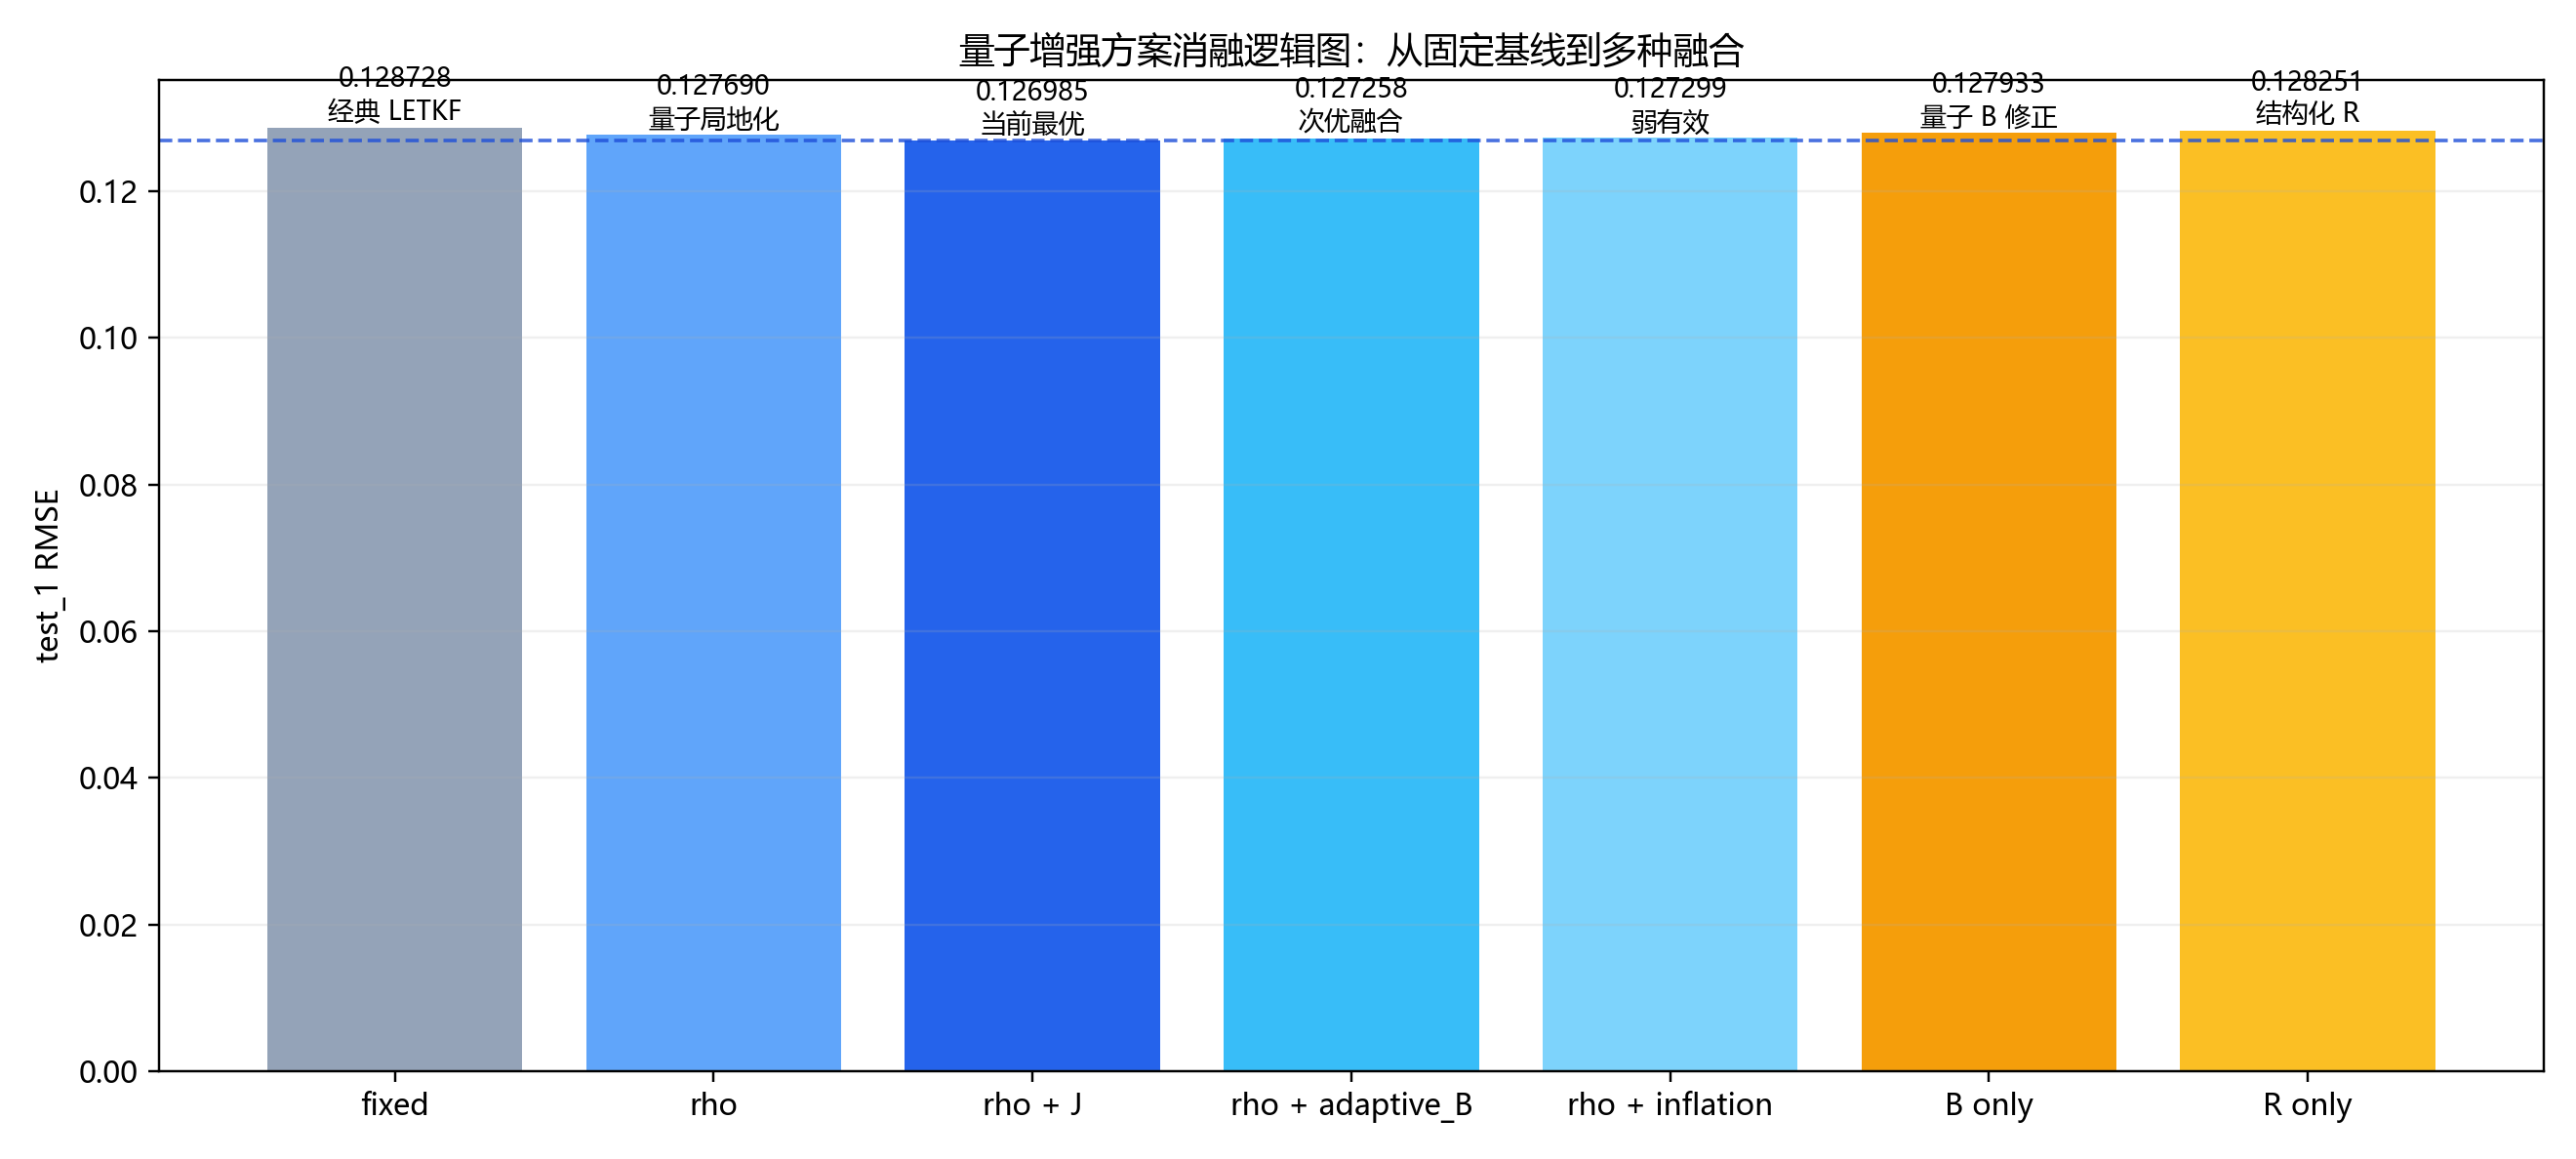
\includegraphics[width=0.92\linewidth]{figures/quantum_ablation_logic.png}
\caption{从经典基线到量子弱融合的整体消融逻辑。}
\label{fig:ablation}
\end{figure}

图 \ref{fig:ablation} 给出了本文的方法推进逻辑。可以看到，我们并不是从一开始就追求复杂的量子替代，而是从经典基线出发，逐步检验量子结构信息的作用位点，并在失败与修正中收敛到当前的弱融合主线。若没有这一步分层验证，量子模块很容易沦为形式化嵌入，既无法解释其作用，也无法稳定复现其收益。

更具体地说，这条推进链可以分成三个阶段。第一阶段是“结构验证”：先确认量子特征映射是否真的能在局地窗口上产生非平凡相似度，而不是随机噪声。第二阶段是“强接入试探”：尝试把量子结构更直接地注入同化权重，观察其是否能成为主导更新信号。第三阶段则是“弱融合收敛”：在确认强接入会退化后，重新设计量子模块的角色，让其只承担温和调制和小幅方向修正的任务。也正是在这一阶段，本文逐步形成了“距离先验保底、量子相似度补充、弱 $J$ 修正后置”的总体框架。

这条实验路线本身也是本文工作量和思考过程的重要组成部分。我们并不是一次性写出最终方案，而是在多轮实验中逐步回答三个问题：量子结构是否存在，量子结构如何进入公式，量子结构进入后为什么会成功或失败。前两个问题决定“能不能做”，第三个问题决定“怎么做才合理”。从最终文本结构上看，后续的建模、算法设计、实验结果和创新点描述，实际上都围绕这三个问题展开。

从论文叙事的角度看，图 \ref{fig:ablation} 的意义不只是展示做过哪些实验，而是说明本文的主线是一条“由失败推动问题收缩”的研究主线。直接接入失败并不是负面结果，恰恰是它告诉我们：量子信号并不适合强行充当主导权重，而更适合作为局地几何修正信号。基于当前受控实验，本文更适合被理解为一份“量子弱融合在 Lorenz96 上的机制验证报告”，而不是一篇已经完成大规模外推的方法论终稿。

\section{建模过程（问题的量子化表示与转化方法）}
本文考虑的动力系统为 $40$ 维 Lorenz96：
\begin{equation}
\frac{dX_j}{dt} = (X_{j+1}-X_{j-2})X_{j-1} - X_j + F.
\end{equation}
观测模型写为
\begin{equation}
y_k = Hx_k + \varepsilon_k, \qquad \varepsilon_k \sim \mathcal{N}(0, R),
\end{equation}
其中 $H$ 为单位观测算子，观测噪声服从高斯分布。设集合规模为 $N_e$，第 $i$ 个状态维度对应的集合扰动向量记为 $\tilde{x}_i\in \mathbb{R}^{N_e}$，局地观测集合记为 $\mathcal{O}_i$，对应的观测扰动矩阵记为 $Y_i\in\mathbb{R}^{N_e\times |\mathcal{O}_i|}$。在经典 LETKF 中，若局地观测逆协方差为 $R_i^{-1}$，则权重空间的分析矩阵写为
\begin{equation}
C_i=\frac{N_e-1}{\lambda_{\mathrm{infl}}}I + Y_i R_i^{-1}Y_i^\top ,
\end{equation}
相应的均值权重与扰动变换矩阵为
\begin{equation}
\bar{w}_i=C_i^{-1}Y_iR_i^{-1}(y_i-\bar{y}_i),\qquad
W_i=\big((N_e-1)C_i^{-1}\big)^{1/2}.
\end{equation}
于是经典 LETKF 在第 $i$ 个维度上的分析均值与扰动分别为
\begin{equation}
\bar{x}^{a}_i=\bar{x}^{f}_i+\tilde{x}_i^\top \bar{w}_i,\qquad
\tilde{x}^{a}_i=\tilde{x}_i^\top W_i.
\end{equation}
本文所有修改都发生在 $R_i^{-1}$ 的构造以及 $\tilde{x}_i$ 的修正方式上，而不改变上述 LETKF 的基本权重空间框架。

为在受限量子资源下引入真实量子信息，本文不对整个 $40$ 维状态进行量子编码，而是将每个局地分析点附近的状态窗口与观测窗口提取为长度为 $4$ 的局地向量，再映射到 $4$ qubits 量子特征空间。设状态窗口为 $s_i$，观测窗口为 $o_j$，则它们经标准化后送入同一量子特征映射电路，得到两个量子态 $\lvert \phi(s_i)\rangle$ 与 $\lvert \phi(o_j)\rangle$。二者之间的量子相似度定义为
\begin{equation}
k_q(i,j)=|\langle \phi(s_i)\mid \phi(o_j)\rangle|^2 .
\end{equation}
该量子相似度反映了局地状态模式与观测模式之间的几何匹配程度。随后，我们不将其直接作为主导权重，而是与经典距离先验结合，构造成弱融合观测权重：
\begin{equation}
w_{ij}\propto \rho_{ij}\big((1-\lambda_\rho)+\lambda_\rho k_q(i,j)\big),
\end{equation}
其中 $\rho_{ij}$ 为经典距离先验，本文按
\begin{equation}
\rho_{ij}\propto 0.1+\exp\!\left(-\frac{d(i,j)^2}{2\sigma^2}\right),\qquad \sigma=\max(r/2,1),
\end{equation}
构造，并在局地窗口内重新归一化为均值为 $1$ 的权重。于是局地观测逆协方差被替换为
\begin{equation}
R_i^{-1}=\mathrm{diag}\!\left(\frac{w_{ij}}{\sigma_{\mathrm{obs}}^2}\right)_{j\in\mathcal{O}_i}.
\end{equation}
这一步清楚表明，本文不是替换 LETKF 的主体公式，而是替换了局地观测加权进入公式的那一层。

这种转化方式的关键意义在于，它把高维状态空间中的复杂建模问题，拆解成一系列局地窗口上的几何匹配问题。量子模块由此不再承担“直接求解全局最优状态”的角色，而是承担“为经典同化器提供局地结构线索”的角色。这种角色转化既符合赛题的量子资源约束，也使量子模块的物理解释更明确。

这里的“局地窗口”并不是单纯为了降维而做的技术处理，而是整个建模思路的核心。Lorenz96 本身具有明显的局地耦合结构，单个状态维度的演化主要受邻近维度影响。因此，如果把整个 $40$ 维状态一次性量子化，不仅资源上不可行，也会掩盖问题本来就具有的局地结构特征。相反，把问题拆解为多个重叠局地窗口后，每个窗口都可以被解释为一个小尺度的“状态模式识别”任务，量子模块在这里更容易发挥几何表示能力。

从建模角度看，本文的关键不是把经典变量机械映射到量子比特上，而是先完成一个问题重述：原问题是“如何在全局状态空间中更新分析场”，重述后变为“如何在每个局地窗口中识别哪些观测模式与当前状态更匹配”。量子特征映射承担的就是这个局地模式识别任务。这样一来，量子模块的输出不再是直接替代分析值，而是为后续的经典更新提供一张局地相似度地图。

\begin{figure}[htbp]
\centering
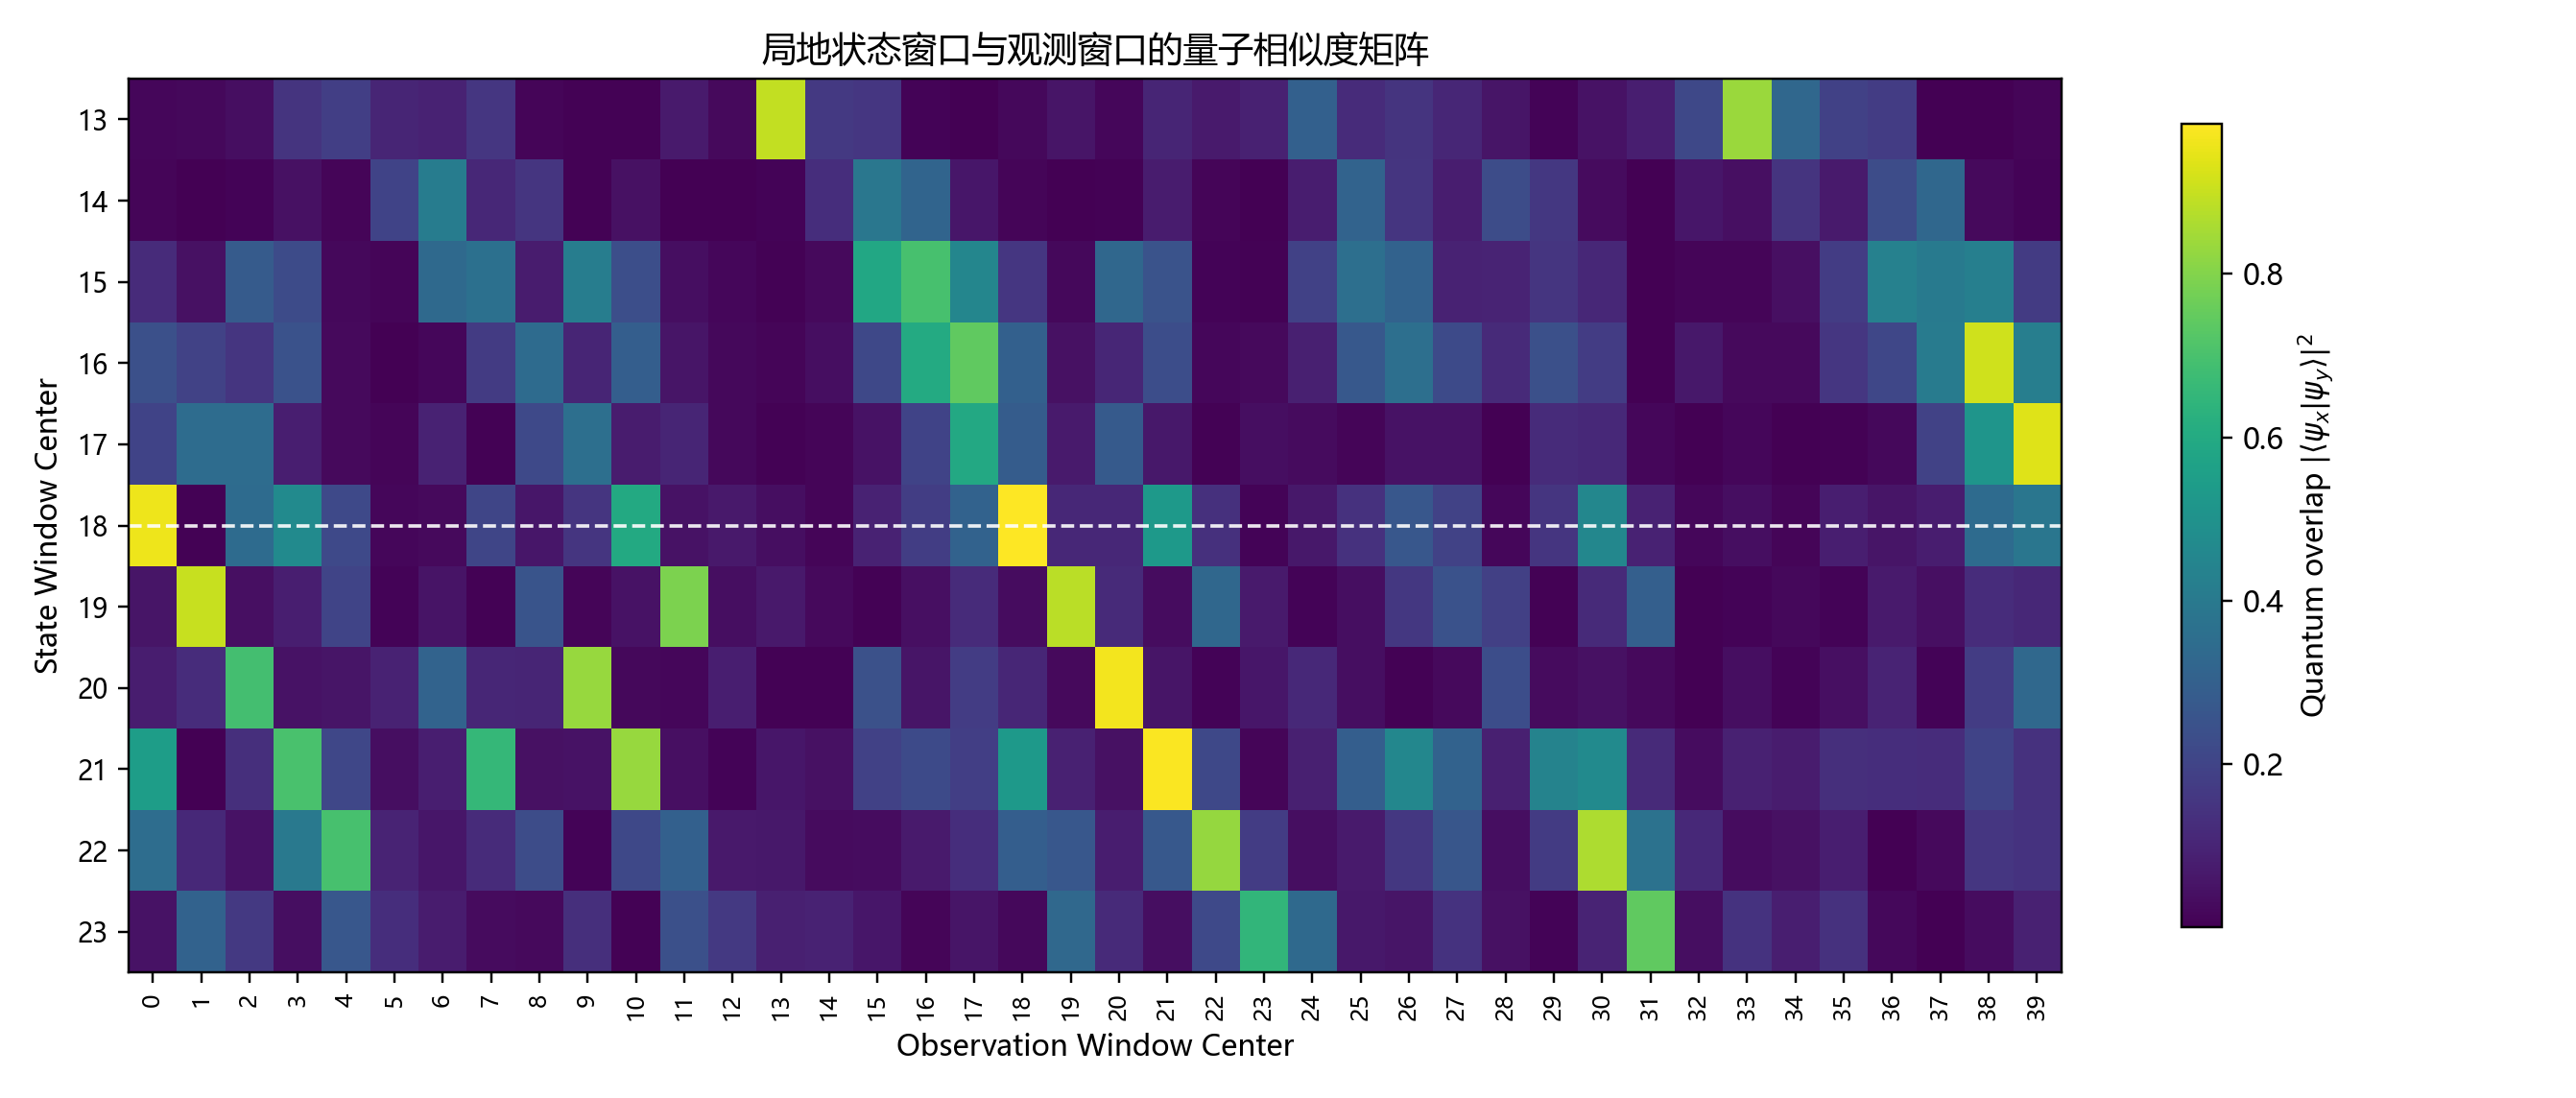
\includegraphics[width=0.92\linewidth]{figures/exp37_quantum_similarity_matrix.png}
\caption{代表性时间步下局地状态窗口与观测窗口之间的量子相似度矩阵。}
\label{fig:qsim}
\end{figure}

图 \ref{fig:qsim} 就是这种建模思想最直接的证据。若量子特征映射只是形式化编码，那么相似度矩阵应当接近随机噪声，缺乏清晰结构；而图中可以看到，相似度在不同窗口之间呈现出明显的强弱差异和局部团块结构。这说明量子特征映射确实捕捉到了状态窗口与观测窗口之间的非平凡几何关系。

更进一步看，图 \ref{fig:qsim} 还有两个重要含义。第一，它说明量子模块提供的不是一个全局统一系数，而是一张随窗口位置变化的结构图谱，这为后续局地加权提供了细粒度依据。第二，它也解释了为什么量子信息不宜直接做全局主导更新：这种相似度本来就是局地的、相对的、随时间变化的，如果把它直接放大到全局公式中，很容易造成过强扰动。因此，本文采用的弱融合建模其实并不是保守妥协，而是对量子相似度性质的自然响应。

除权重修正外，本文还对集合扰动方向引入一个弱 $J$ 修正。设量子权重归一化后得到 $q_i\in \mathbb{R}^{|\mathcal{O}_i|}$，则局地观测模式定义为
\begin{equation}
m_i=\frac{Y_i q_i-\mathrm{mean}(Y_i q_i)\mathbf{1}}{\|Y_i q_i-\mathrm{mean}(Y_i q_i)\mathbf{1}\|_2+\varepsilon}.
\end{equation}
再定义局地耦合系数
\begin{equation}
c_i=\frac{\langle \tilde{x}_i,m_i\rangle}{\|\tilde{x}_i\|_2+\varepsilon},
\end{equation}
并据此构造
\begin{equation}
J_i=c_i m_i,\qquad \tilde{x}_i^{(J)}=\tilde{x}_i+\lambda_J J_i .
\end{equation}
当前 exp37 受控实验并未额外引入硬门控阈值，等价于取门控变量 $g_i\equiv 1$；修正强度完全由 $c_i$ 与 $\lambda_J$ 决定。这一点需要特别说明，因为本文后续只讨论当前实验脚本对应的弱修正版本，而不把后续 gated 变体混入同一组结果表中。

因此，最终用于分析更新的公式为
\begin{equation}
\bar{x}^{a}_i=\bar{x}^{f}_i+(\tilde{x}_i^{(J)})^\top \bar{w}_i,\qquad
\tilde{x}^{a}_i=(\tilde{x}_i^{(J)})^\top W_i.
\end{equation}
基于上述分析，本文的建模过程可以概括为三步：首先利用 Lorenz96 的局地耦合结构把高维问题分解为多个局地窗口；其次在每个窗口上通过量子特征映射构造状态--观测相似度；最后再以“弱加权 + 弱方向修正”的方式把量子结构送入 LETKF。这样得到的模型既保留了经典同化的稳定性，也使读者能够明确看到本文相对于经典基线到底改动了哪一层、如何改动以及为什么必须弱改动。

\section{量子算法设计（算法原理、步骤与伪代码）}
\subsection{算法原理}
本文算法由两部分组成：经典部分使用 LETKF 完成集合传播与局地分析；量子部分负责生成局地相似度，用于调制局地观测权重，并对集合扰动方向施加由局地耦合系数控制的弱 $J$ 修正。其设计思想是：让量子模块提供结构信息，而不是替代整个同化器。

\begin{figure}[htbp]
\centering
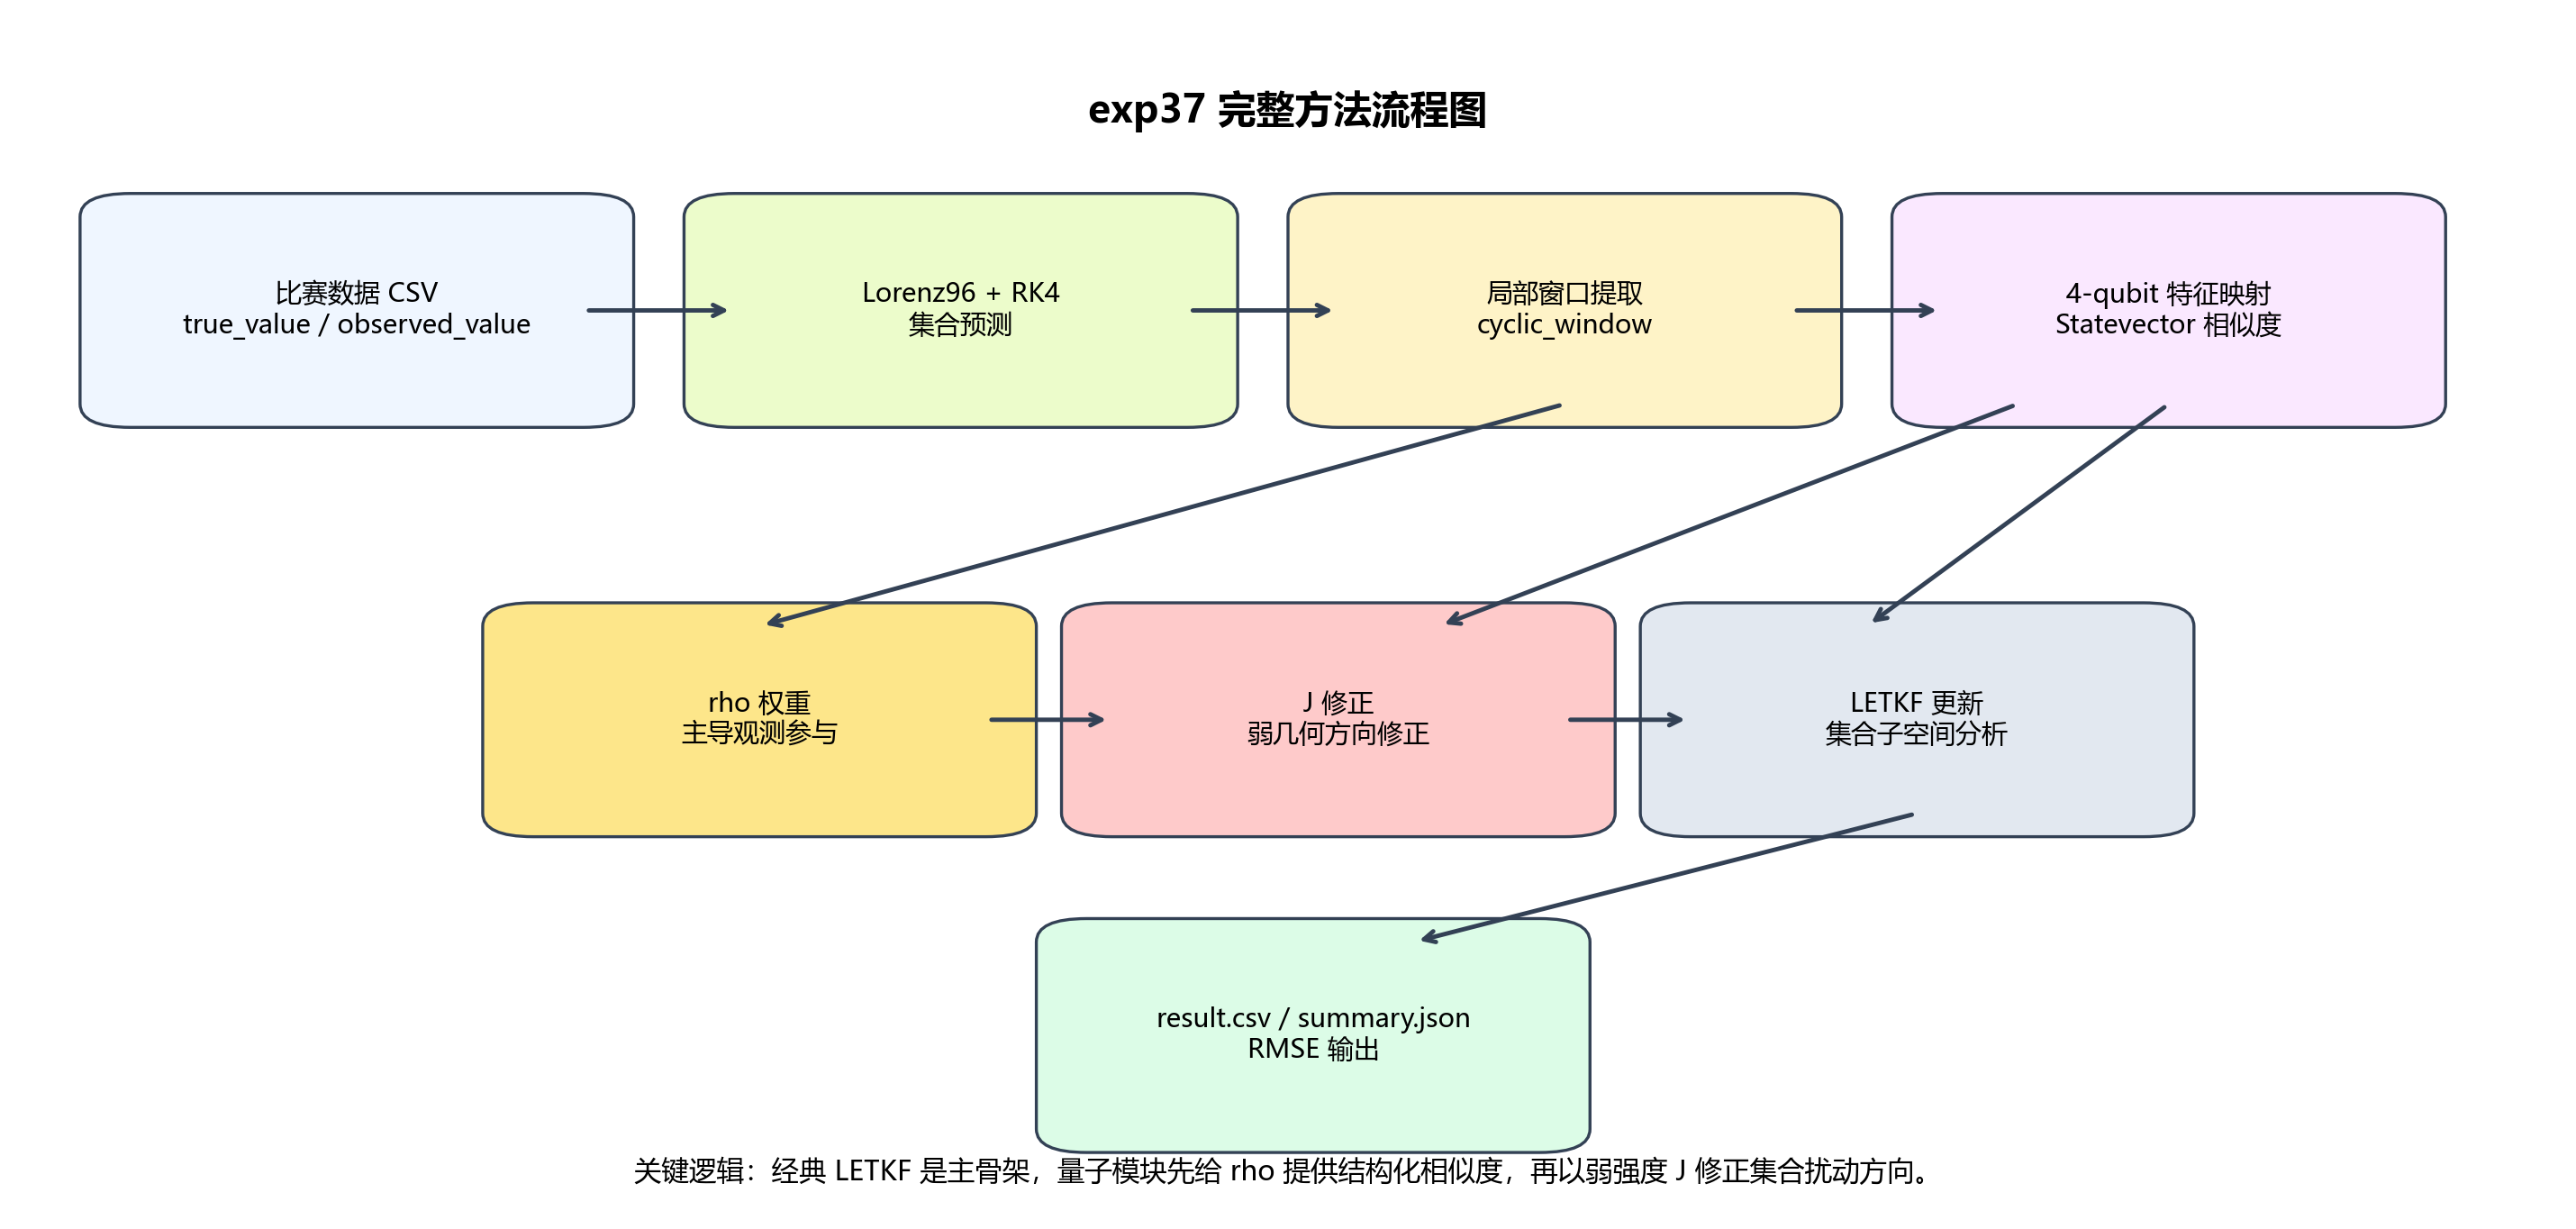
\includegraphics[width=0.9\linewidth]{figures/exp37_method_flowchart.png}
\caption{从输入数据到量子相似度、再到 LETKF 更新的整体流程。}
\label{fig:flow}
\end{figure}

图 \ref{fig:flow} 展示了算法的完整数据流。量子模块只负责构造局地相似度与方向信息，真正的状态更新仍由经典 LETKF 完成，这也是本文保持稳定性的关键。也正因为如此，本文的方法重点不是“让量子模块做更多事情”，而是“让量子模块在最合适的地方介入”。

图 \ref{fig:flow} 还揭示了一个常被忽略的事实：本文算法不是把量子模块附着在流程末端做后处理，而是把它安放在局地权重形成与扰动方向修正之间的关键位置。这个位置选择非常重要。若量子模块放在更外层，它只能扮演参数搜索器；若放在更内层并直接主导分析更新，又容易造成不稳定。将其放在“局地结构判别”这一中间层，既能发挥量子表示能力，又不会破坏经典同化器的主更新机制。

\begin{figure}[htbp]
\centering
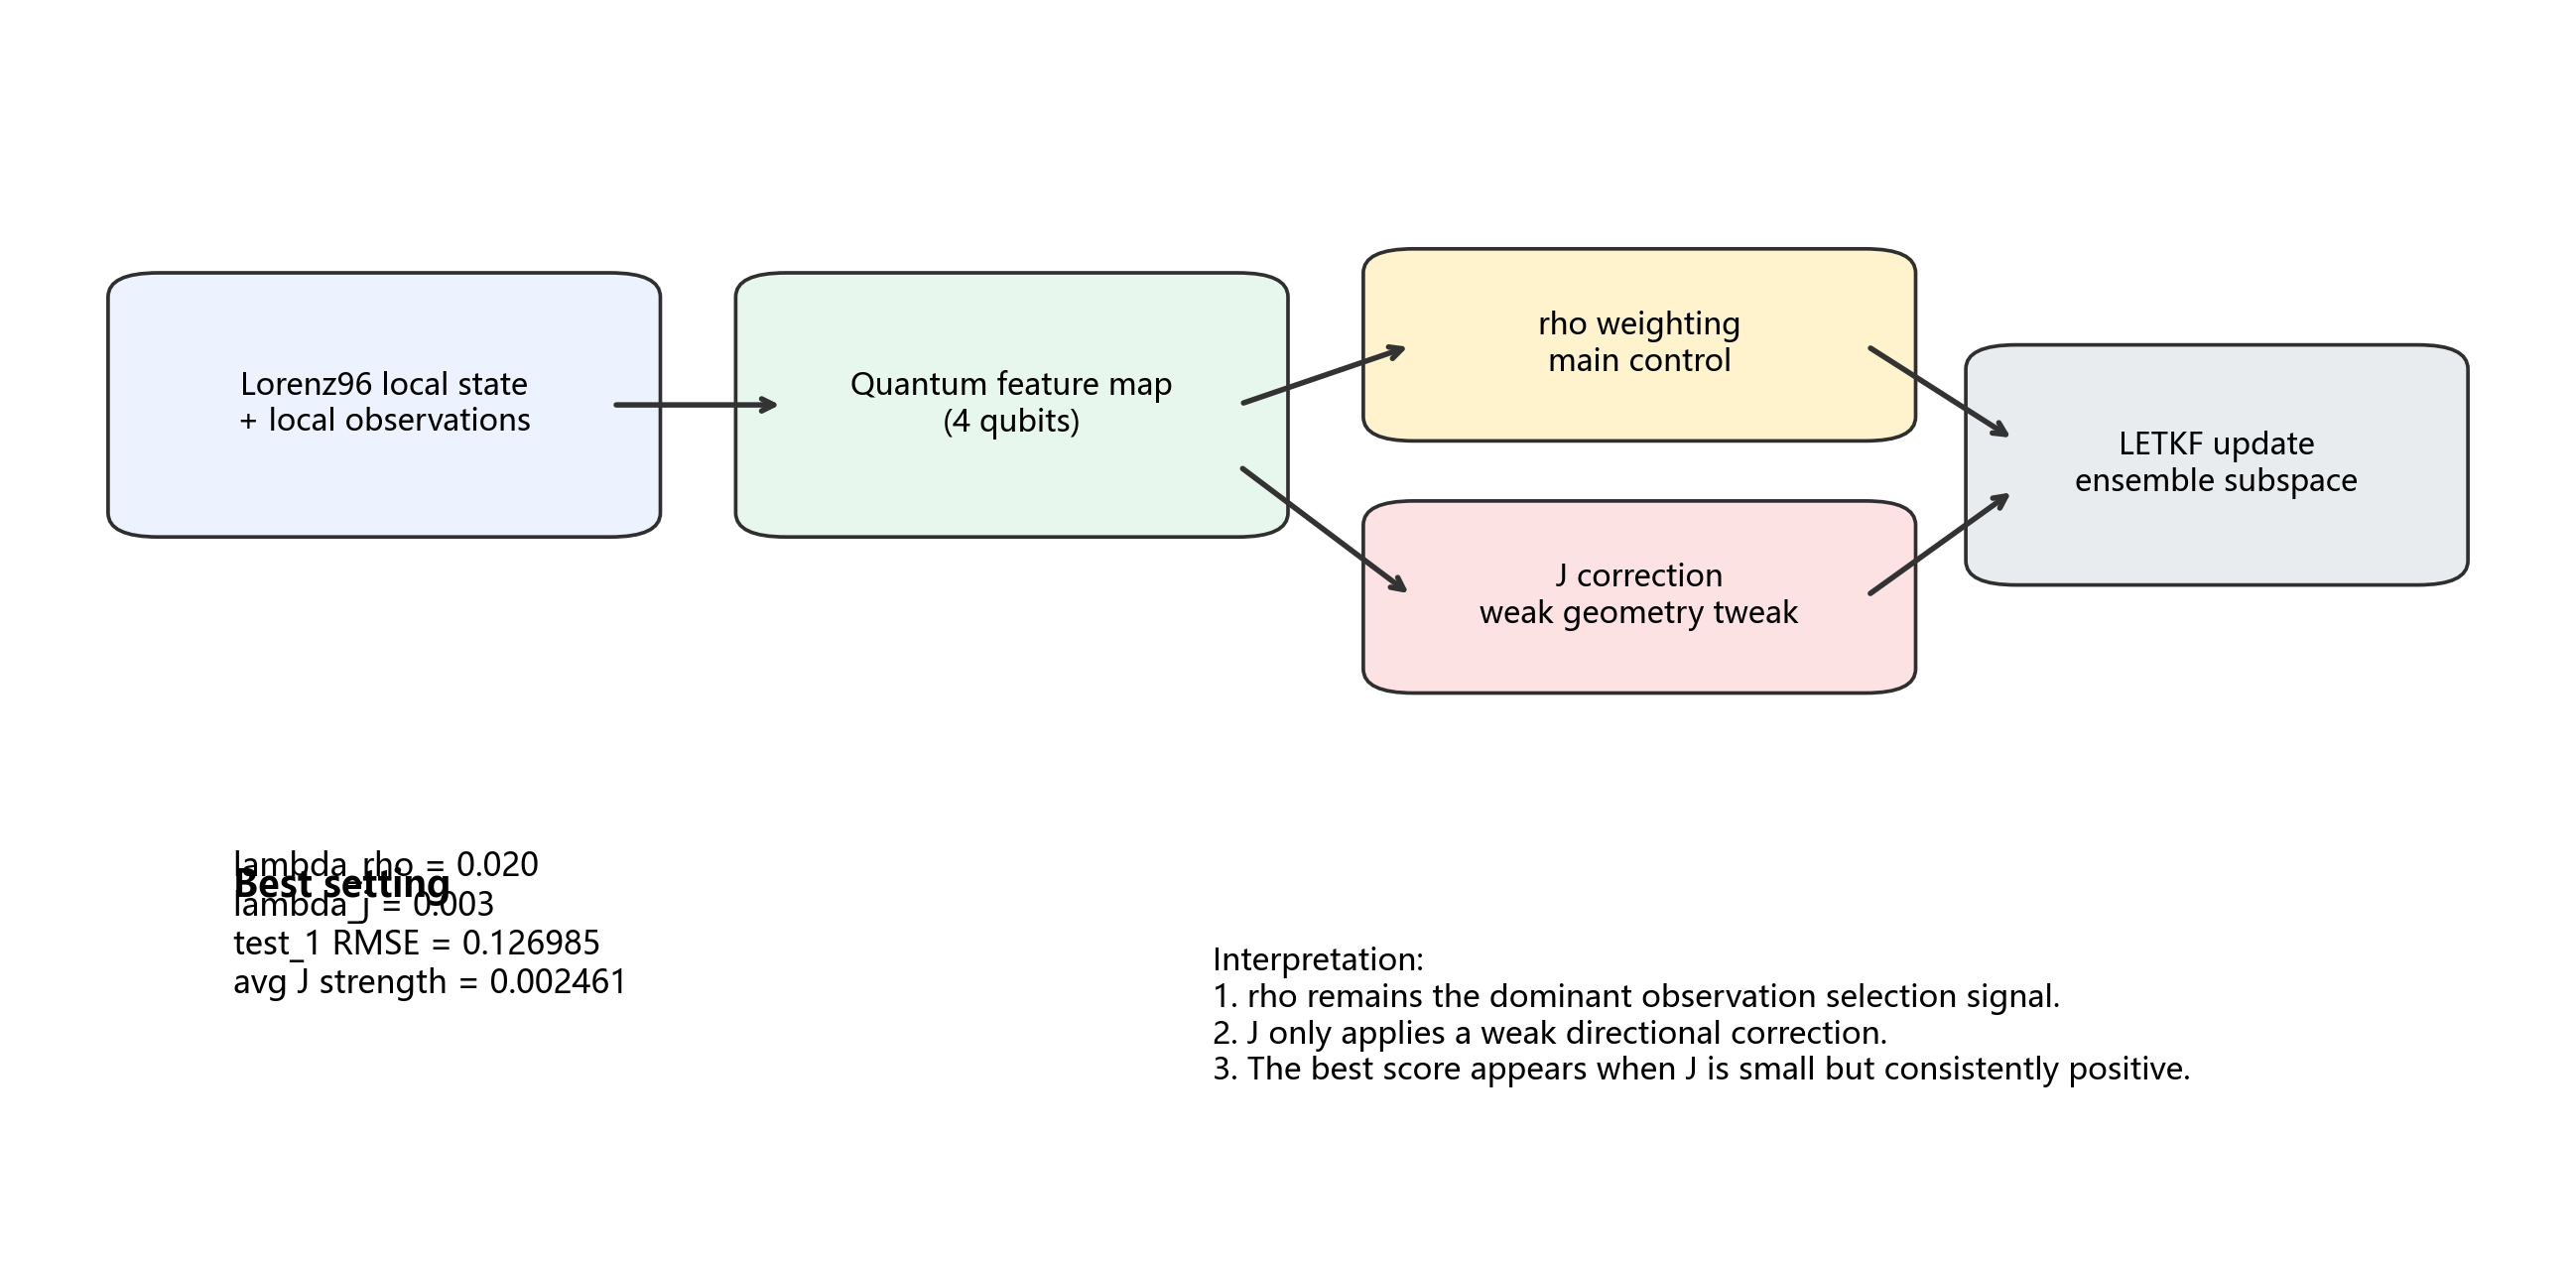
\includegraphics[width=0.92\linewidth]{figures/exp37_method_schematic.png}
\caption{exp37 方法结构示意图，展示 $\rho$ 主导与 $J$ 弱修正的接入关系。}
\label{fig:method}
\end{figure}

图 \ref{fig:method} 比流程图更进一步，它把本文算法最核心的控制思想展示了出来：$\rho$ 融合负责提供主要的局地观测加权，而 $J$ 修正只做小幅方向性调节。也就是说，本文并不是同时把多个量子信号大幅注入更新公式，而是建立了“主调制 + 弱修正”的双层结构。这个结构的优点在于，一旦某个局地窗口上的量子信号不够稳定，损害也会被限制在弱修正层，而不会直接冲击整个分析更新。

为避免口号化叙述，这里把算法中最关键的三个量重新明确写出。第一，局地量子融合权重为
\begin{equation}
w_{ij}=\mathrm{Norm}\!\left(\rho_{ij}\big((1-\lambda_\rho)+\lambda_\rho k_q(i,j)\big)\right),
\end{equation}
其中 $\mathrm{Norm}(\cdot)$ 表示裁剪后再归一化到均值为 $1$ 的操作。第二，局地模式为
\begin{equation}
m_i=\mathrm{NormVec}(Y_i q_i),
\end{equation}
其中 $q_i$ 由量子相似度矩阵得到。第三，$J$ 修正项为
\begin{equation}
J_i=c_i m_i,\qquad c_i=\frac{\langle \tilde{x}_i,m_i\rangle}{\|\tilde{x}_i\|_2+\varepsilon},
\end{equation}
并据此得到修正后的扰动
\begin{equation}
\tilde{x}_i^{(J)}=\tilde{x}_i+\lambda_J J_i.
\end{equation}
当前 exp37 脚本没有额外硬门控条件，等价于使用连续耦合系数 $c_i$ 作为内生强度控制；因此本文报告中的“弱 $J$ 修正”应理解为连续弱修正，而不是阈值门控修正。后续 gated 变体属于扩展实验，不纳入本报告主结果表。

\subsection{算法步骤}
\begin{itemize}
\item 用观测初始化集合，并按 Lorenz96 动力学推进每个集合成员；
\item 对每个状态维度提取局地状态窗口和局地观测窗口；
\item 通过量子特征映射计算状态窗口与各观测窗口之间的量子相似度；
\item 将量子相似度与距离先验进行弱融合，形成局地观测权重；
\item 利用局地量子模式与集合扰动的耦合系数构造连续弱 $J$ 修正；
\item 用修正后的局地权重和扰动信号执行 LETKF 分析更新。
\end{itemize}

上述流程中，最重要的不是单个公式本身，而是“先加权、再弱修正”的顺序。我们先让量子相似度温和调节观测权重，再利用局地模式耦合关系修正集合方向，这样可以避免量子信息一次性过强进入更新公式，引发数值不稳定。

这一顺序实际上对应了本文对量子信号可信度的分层判断。观测权重调制属于相对温和的介入，因为它仍然保留经典距离先验作为底座；而集合方向修正则更敏感，因为它直接影响分析增量的几何方向。因此，本文把方向修正限制为与耦合系数 $c_i$ 和 $\lambda_J$ 成正比的小幅连续修正，而不是直接替换整个更新方向。这种“分层介入、逐步放权”的策略，是本文从前期失败实验中总结出来的重要经验。

\subsection{伪代码}
\noindent\textbf{算法 1：量子弱融合 LETKF}
\begin{quote}
\small\ttfamily
输入：观测序列 $y_{1:T}$，集合规模 $N$，局地半径 $r$，融合系数 $\lambda_\rho,\lambda_J$\\
初始化集合 $E_0$\\
for $t=1$ to $T$ do\\
\quad 用 Lorenz96 推进每个集合成员\\
\quad for 每个状态维度 $i$ do\\
\qquad 提取状态窗口 $s_i$ 与局地观测窗口集合 $\{o_j\}$\\
\qquad 计算量子相似度 $k_q(i,j)$\\
\qquad 计算弱融合权重 $w_{ij}$\\
\qquad 构造局地量子模式 $m_q$\\
\qquad 计算耦合系数 $c_i$，得到 $J_i=c_i m_q$\\
\qquad 构造修正后扰动 $\tilde{x}_i^{(J)}=\tilde{x}_i+\lambda_J J_i$\\
\qquad 用 $w_{ij}$ 和修正后的扰动执行 LETKF 更新\\
\quad end for\\
\quad 输出当前分析场均值\\
end for
\end{quote}

从伪代码可以看出，本文算法并非简单在 LETKF 前后插入一个量子黑箱，而是把量子相似度计算、弱融合权重构造、局地模式提取、$J$ 修正构造和分析更新整合为一条连续的数据流。这样的设计使算法具备两个优点。第一，每一步都可以单独解释和可视化，因此方法不是黑箱。第二，每一步都可以单独消融和替换，因此本文的实验路线天然支持解释性验证和机制分析，而不仅仅是最终指标比较。

\section{量子线路实现}
本文采用 $4$ qubits 参数化量子特征映射电路。对每个局地窗口特征，先通过 Hadamard 门与单比特旋转门建立基本编码，再使用相邻量子比特之间的受控相位和旋转门刻画局地分量之间的耦合关系。该设计具有两点优势：其一，线路规模固定、资源开销低，满足赛题比特限制；其二，线路表达的是局地几何关系，便于与 LETKF 的局地分析思想对应。

量子相似度由量子态重叠直接给出，不需要额外训练大型量子模型，因此实现简单且可复现。当前方案中单次量子线路仅使用 $4$ 个量子比特，远低于赛题规定的 $30$ qubits 上限。

\begin{figure}[htbp]
\centering
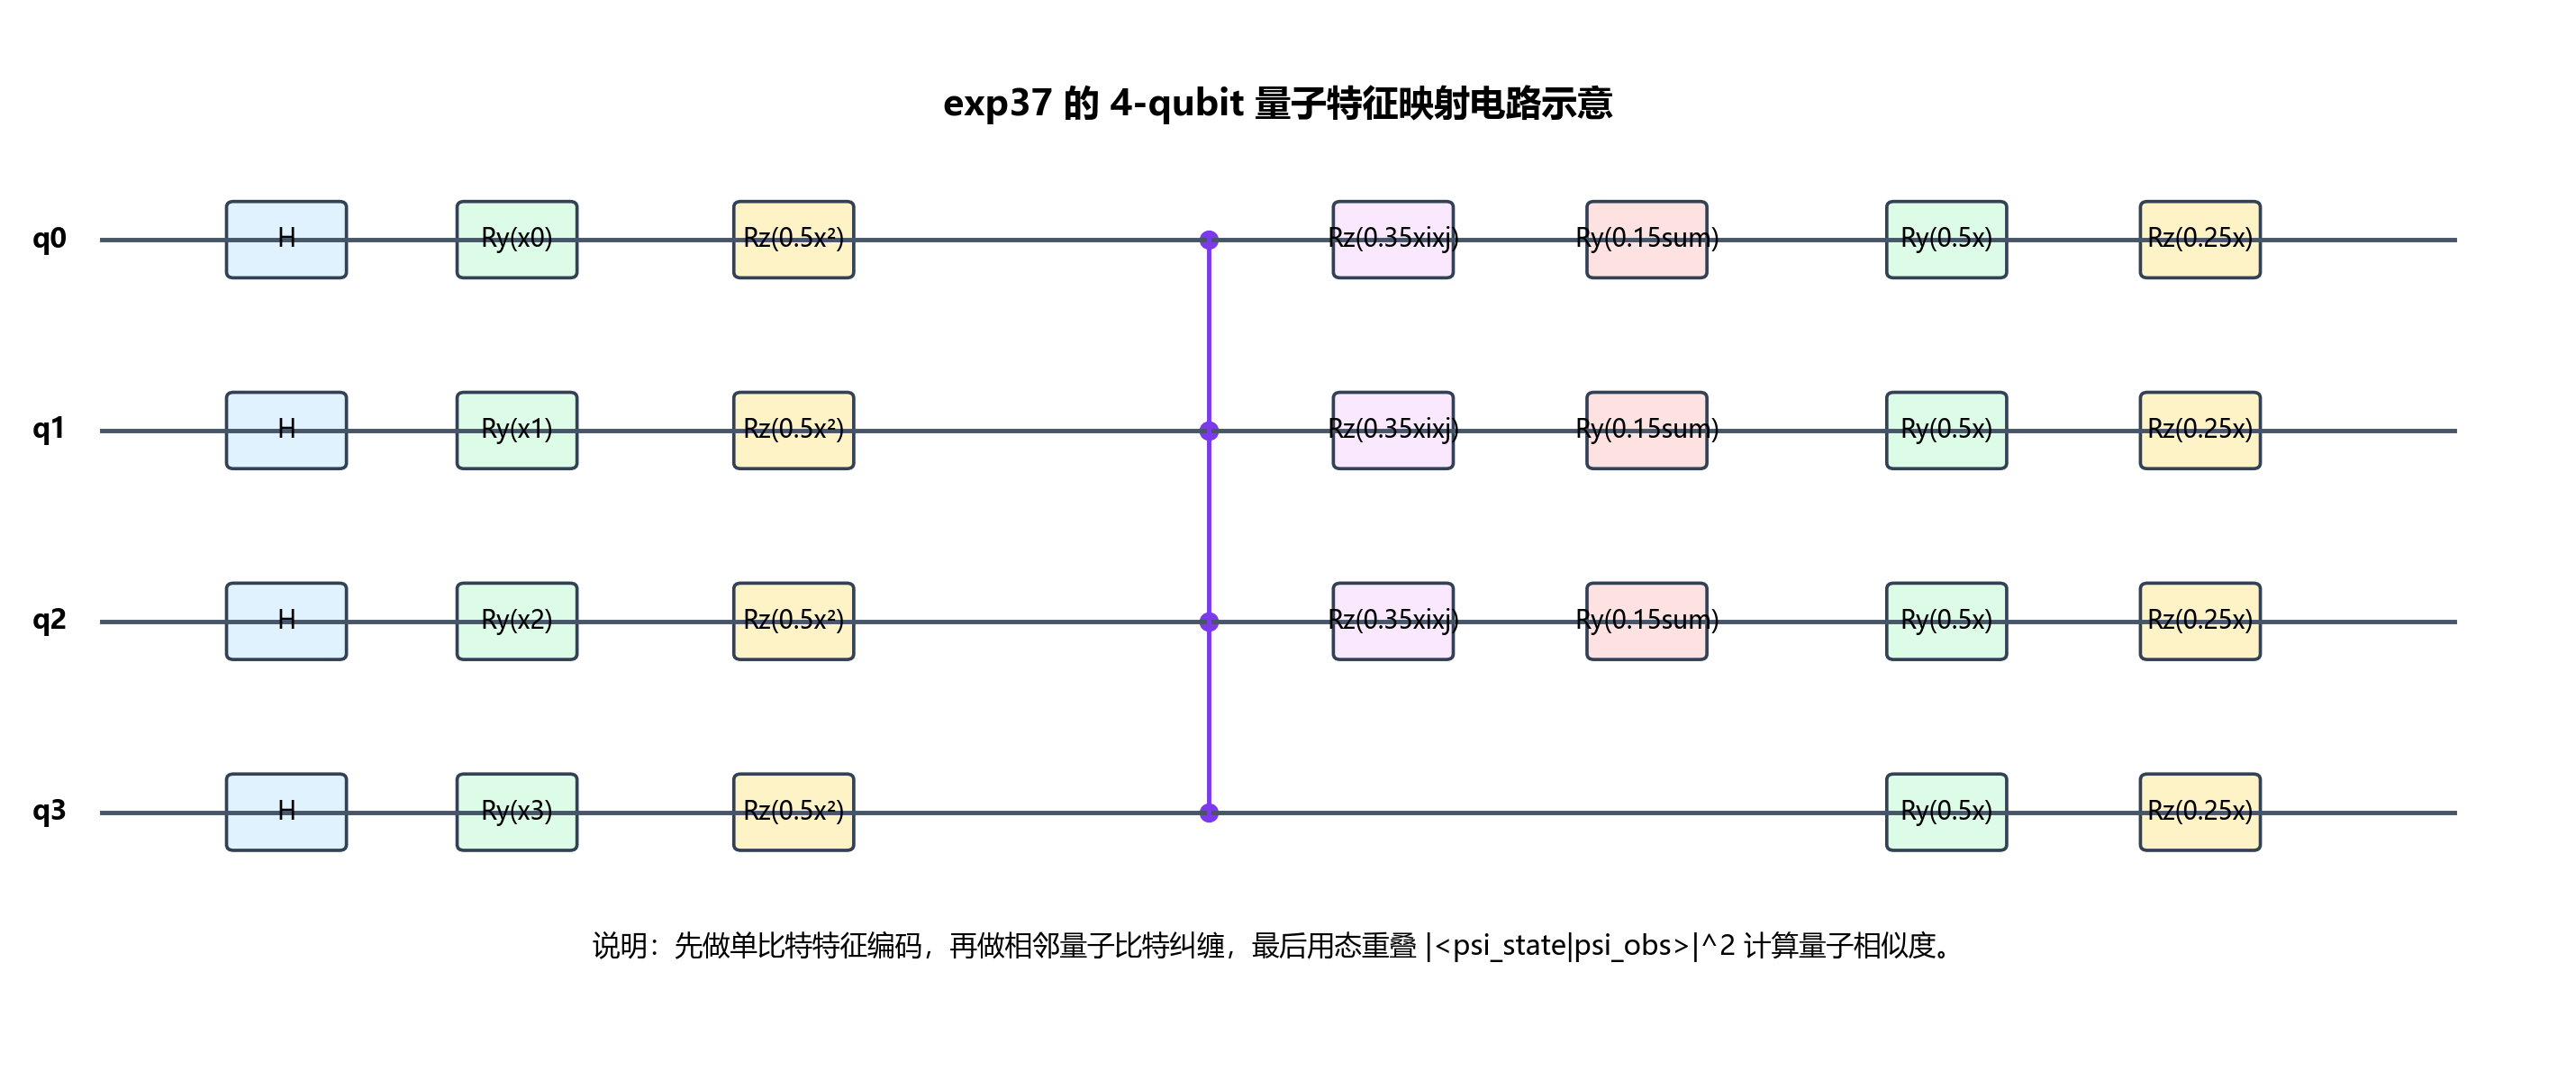
\includegraphics[width=0.82\linewidth]{figures/exp37_quantum_circuit_schematic.png}
\caption{4-qubit 量子特征映射电路示意。}
\label{fig:circuit}
\end{figure}

图 \ref{fig:circuit} 表明当前方案只使用 $4$ qubits 的浅层线路即可完成局地结构编码，因此在资源层面具有明显优势。与需要更深层电路或更大量子比特的方案相比，这种实现更适合在受限模拟环境中稳定运行，也更容易解释不同门结构对局地模式表达的作用。

更重要的是，图 \ref{fig:circuit} 使“可解释性”不再停留在算法层面，而落实到了线路层面。线路前半部分的单比特编码负责把局地窗口中的数值特征转入量子态，后半部分的相邻耦合门则负责表达局地分量之间的关系。这意味着本文并不是任意选了一条量子线路来满足赛题要求，而是让线路结构与局地几何建模目标保持一致。也正因为电路浅、结构清晰，我们才有可能把后续的量子相似度矩阵、权重变化和 $J$ 修正联系起来做解释。

\begin{figure}[htbp]
\centering
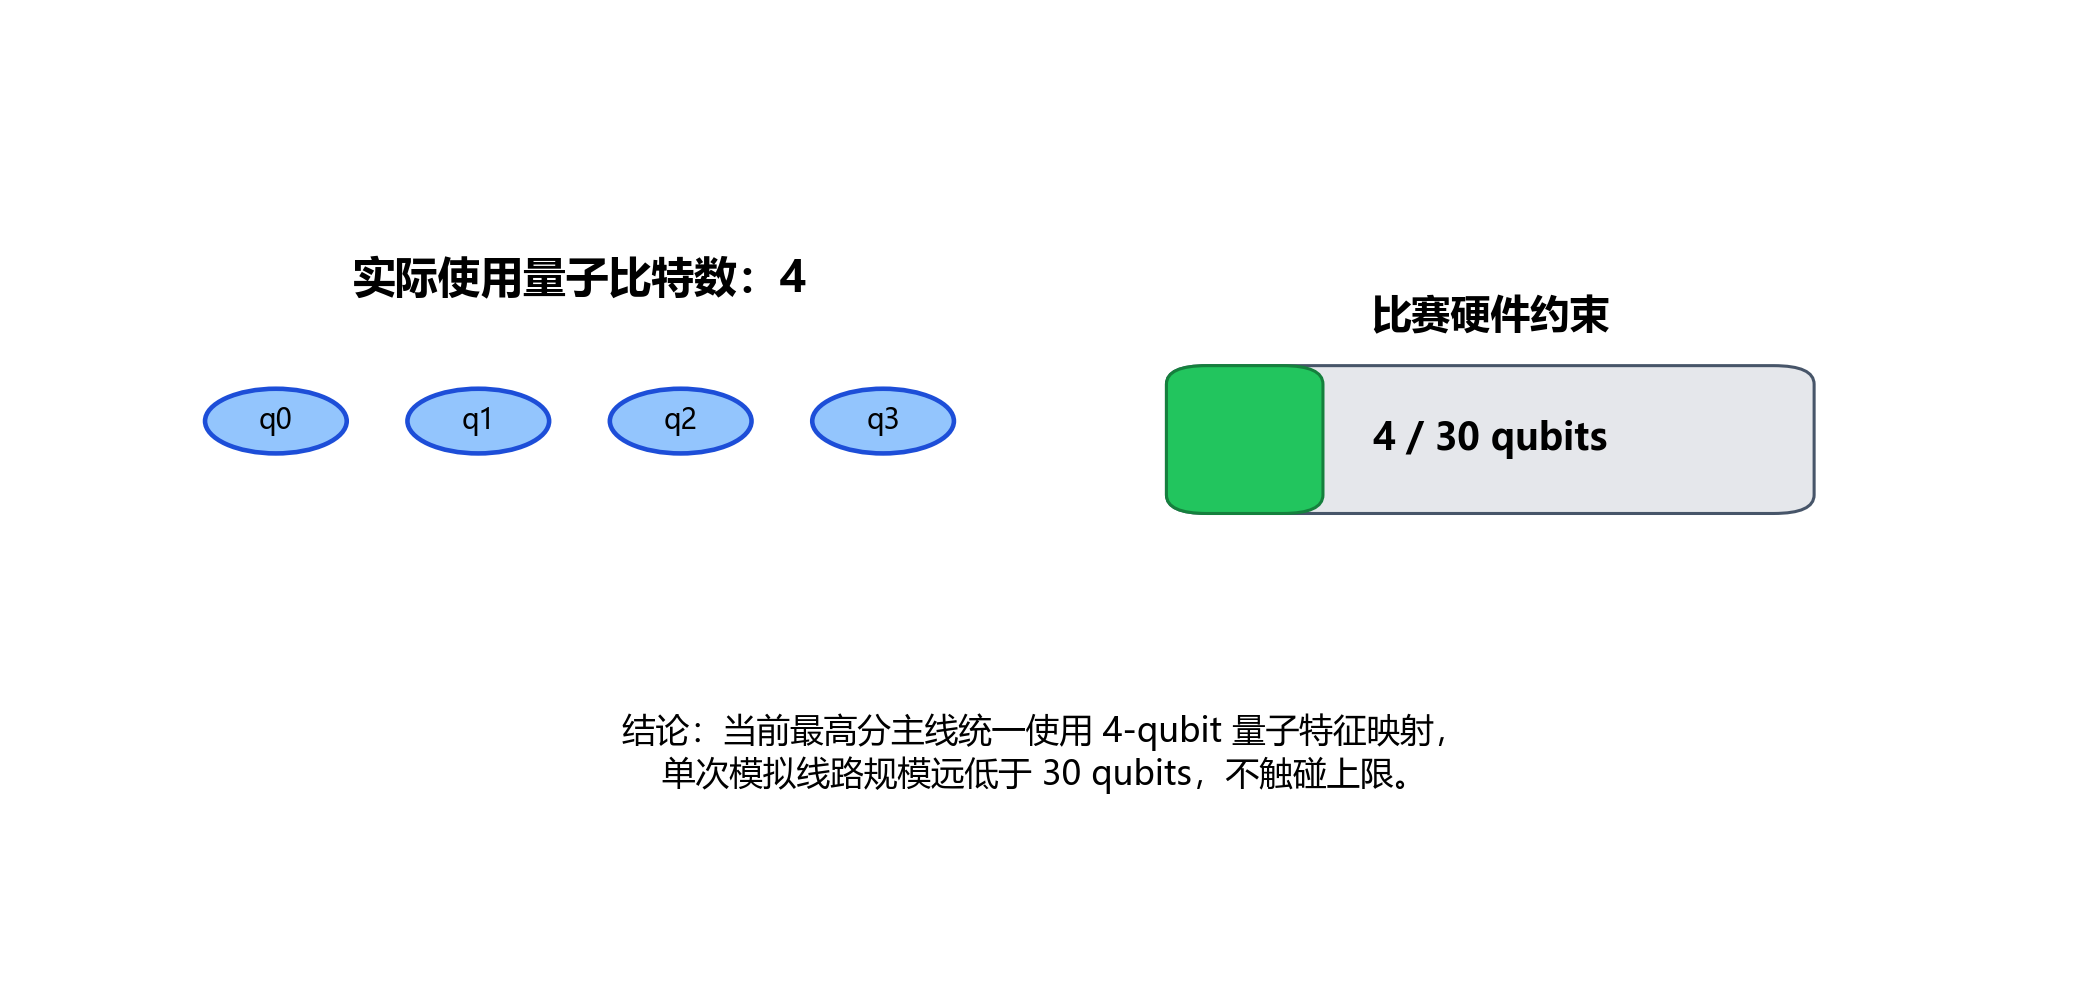
\includegraphics[width=0.88\linewidth]{figures/quantum_qubit_compliance.png}
\caption{当前方案的量子比特使用量与赛题上限对比。}
\label{fig:qubits}
\end{figure}

图 \ref{fig:qubits} 则从资源合规性的角度补充了另一层说明。当前方案仅使用 $4$ qubits，远低于赛题要求的 $30$ qubits 上限，这说明本文并不是依赖大规模量子资源“堆”出结果，而是在严格受限的线路规模下，通过局地建模与结构化融合获得增益。对评委而言，这一点非常关键，因为它证明方案具有真实的工程可实施性，而不是只在理想化资源条件下成立。

从整体上看，本节两张图分别回答了两个问题：图 \ref{fig:circuit} 回答“线路是怎么工作的”，图 \ref{fig:qubits} 回答“线路为什么合规且现实可行”。前者支撑可解释性，后者支撑工程可交付性。两者结合，才能完整说明本文所采用的量子线路不仅存在，而且是为本任务量身设计、可以实际运行且便于分析的。

\section{实验结果与展示（使用最终验证数据集得到的结果及可视化）}
\subsection{实验设置}
本文所报告的主结果对应 `exp37` 受控实验脚本，其固定设置为：ensemble size $N_e=40$，inflation 系数 $\lambda_{\mathrm{infl}}=1.02$，观测噪声标准差 $\sigma_{\mathrm{obs}}=0.5$，Lorenz96 时间步长 $\Delta t=0.05$，外强迫项 $F=8.0$，随机种子为 $2$，局地支持半径为 $20$，局地窗口长度为 $4$，量子线路使用 $4$ qubits。当前受控实验在 `train` 与 `test\_1` 两个 split 上运行，不额外设置独立验证集；因此，本文所有“最优配置”都应理解为在当前报告设定下的最优记录，而不是已经完成严格泛化验证的最终方法结论。

在该脚本中，量子弱融合参数网格仅包含四组配置：
\begin{equation}
(\lambda_\rho,\lambda_J)\in\{(0.02,0.003),(0.02,0.005),(0.03,0.003),(0.03,0.005)\}.
\end{equation}
因此，本节的对比范围是透明且有限的：`fixed`、`corr` 与四组 `rho\_j\_weak\_fusion` 变体。这一设定的优点是便于做受控比较，缺点是搜索范围仍然较窄；我们在结论中将据此保持较谨慎的表述。

\subsection{系统性消融与最优配置来源}

\begin{table}[htbp]
\centering
\caption{exp37 全部受控配置的 train/test\_1 结果与平均 $J$ 修正强度}
\label{tab:ablation}
\begin{tabular}{lcccc}
\toprule
方法 & $\lambda_\rho$ & $\lambda_J$ & test\_1 RMSE & avg $J$ strength \\
\midrule
fixed & -- & -- & 0.12873 & -- \\
corr & -- & -- & 0.14279 & -- \\
rho\_j\_weak\_fusion & 0.02 & 0.003 & 0.12698 & 0.00246 \\
rho\_j\_weak\_fusion & 0.02 & 0.005 & 0.12724 & 0.00408 \\
rho\_j\_weak\_fusion & 0.03 & 0.003 & 0.12706 & 0.00246 \\
rho\_j\_weak\_fusion & 0.03 & 0.005 & 0.12745 & 0.00409 \\
\bottomrule
\end{tabular}
\end{table}

表 \ref{tab:ablation} 给出了本次 exp37 受控实验中全部六组配置的结果。可以看到，四组量子弱融合配置全部优于 `fixed`，而 `corr` 明显退化。这一点非常重要，因为它说明本文并不是“从很多实验里挑了一个最好看的结果”，而是在当前公开列出的全部参数网格内，量子弱融合整体上都优于直接相关性加权，并稳定压过经典 `fixed` 基线。其中最优配置为 $(\lambda_\rho,\lambda_J)=(0.02,0.003)$，其 test\_1 RMSE 为 $0.12698$，相对 `fixed` 的 $0.12873$ 下降约 $1.35\%$，相对 `corr` 的 $0.14279$ 下降约 $11.07\%$。与此同时，表中还可以看到，平均 $J$ 修正强度从约 $0.00246$ 提高到约 $0.00409$ 时，test\_1 RMSE 反而变差，这为“弱修正优于强修正”提供了直接证据。

\subsection{主结果}
在系统性消融的基础上，表 \ref{tab:main-result} 仅把最具代表性的三类方法提炼出来：经典稳定基线 `fixed`、直接结构化加权 `corr`，以及当前最优的量子弱融合配置。

\begin{figure}[htbp]
\centering
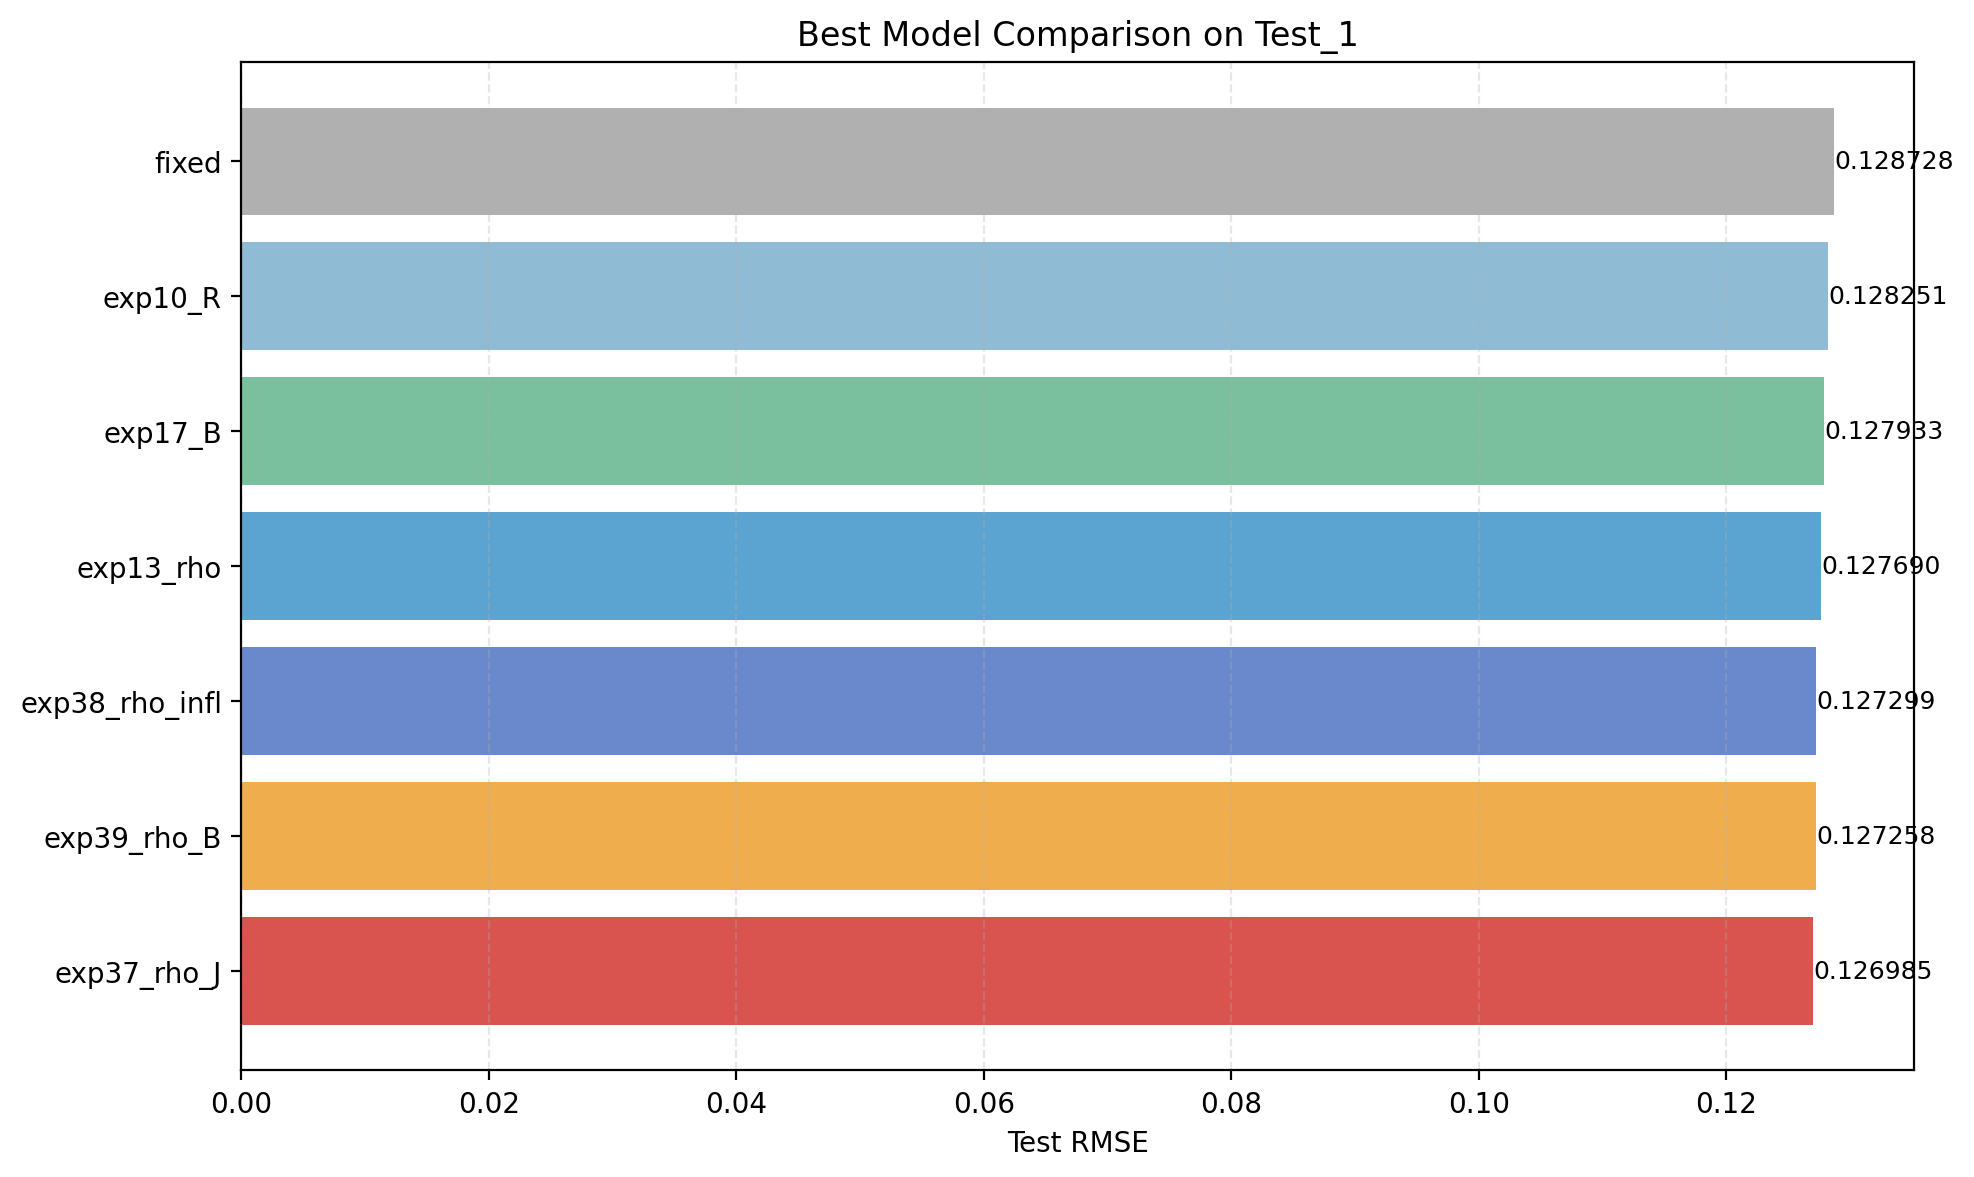
\includegraphics[width=0.88\linewidth]{figures/best_model_rmse_comparison.png}
\caption{当前主线方法与基线方法的 test\_1 RMSE 对比。}
\label{fig:best-rmse}
\end{figure}

\begin{table}[t]
\centering
\caption{test\_1 上的主要结果对比}
\label{tab:main-result}
\begin{tabular}{lcc}
\toprule
方法 & RMSE & MAE \\
\midrule
fixed & 0.12873 & 0.08922 \\
corr & 0.14279 & 0.10202 \\
量子弱融合最优（$\lambda_\rho=0.02,\lambda_J=0.003$） & 0.12698 & 0.08799 \\
\bottomrule
\end{tabular}
\end{table}

结果显示，直接相关性加权会明显退化，而量子弱融合方案相对 fixed 基线取得了稳定的小幅提升。图 \ref{fig:best-rmse} 从总体 RMSE 角度说明最优量子方案优于经典 fixed；更重要的是，量子弱融合的优势并不是孤立单点，而是建立在表 \ref{tab:ablation} 的完整参数网格基础上。因此，图 \ref{fig:best-rmse} 回答的问题不是“有没有一个好看的最优点”，而是“在当前受控实验里，是否存在稳定优于经典基线的量子接入方式”。答案是肯定的，但优势幅度目前仍然属于受控场景下的温和增益，而非数量级跃升。

仅看表 \ref{tab:main-result} 和图 \ref{fig:best-rmse} 还不足以说明方法为什么有效，因此下面继续从误差分布、时间稳定性、空间分布以及具体状态切片四个角度做展开分析。这样的安排也是为了避免把结果部分写成单纯的“指标罗列”，而是把量子弱融合究竟改善了什么说清楚。

\begin{figure}[htbp]
\centering
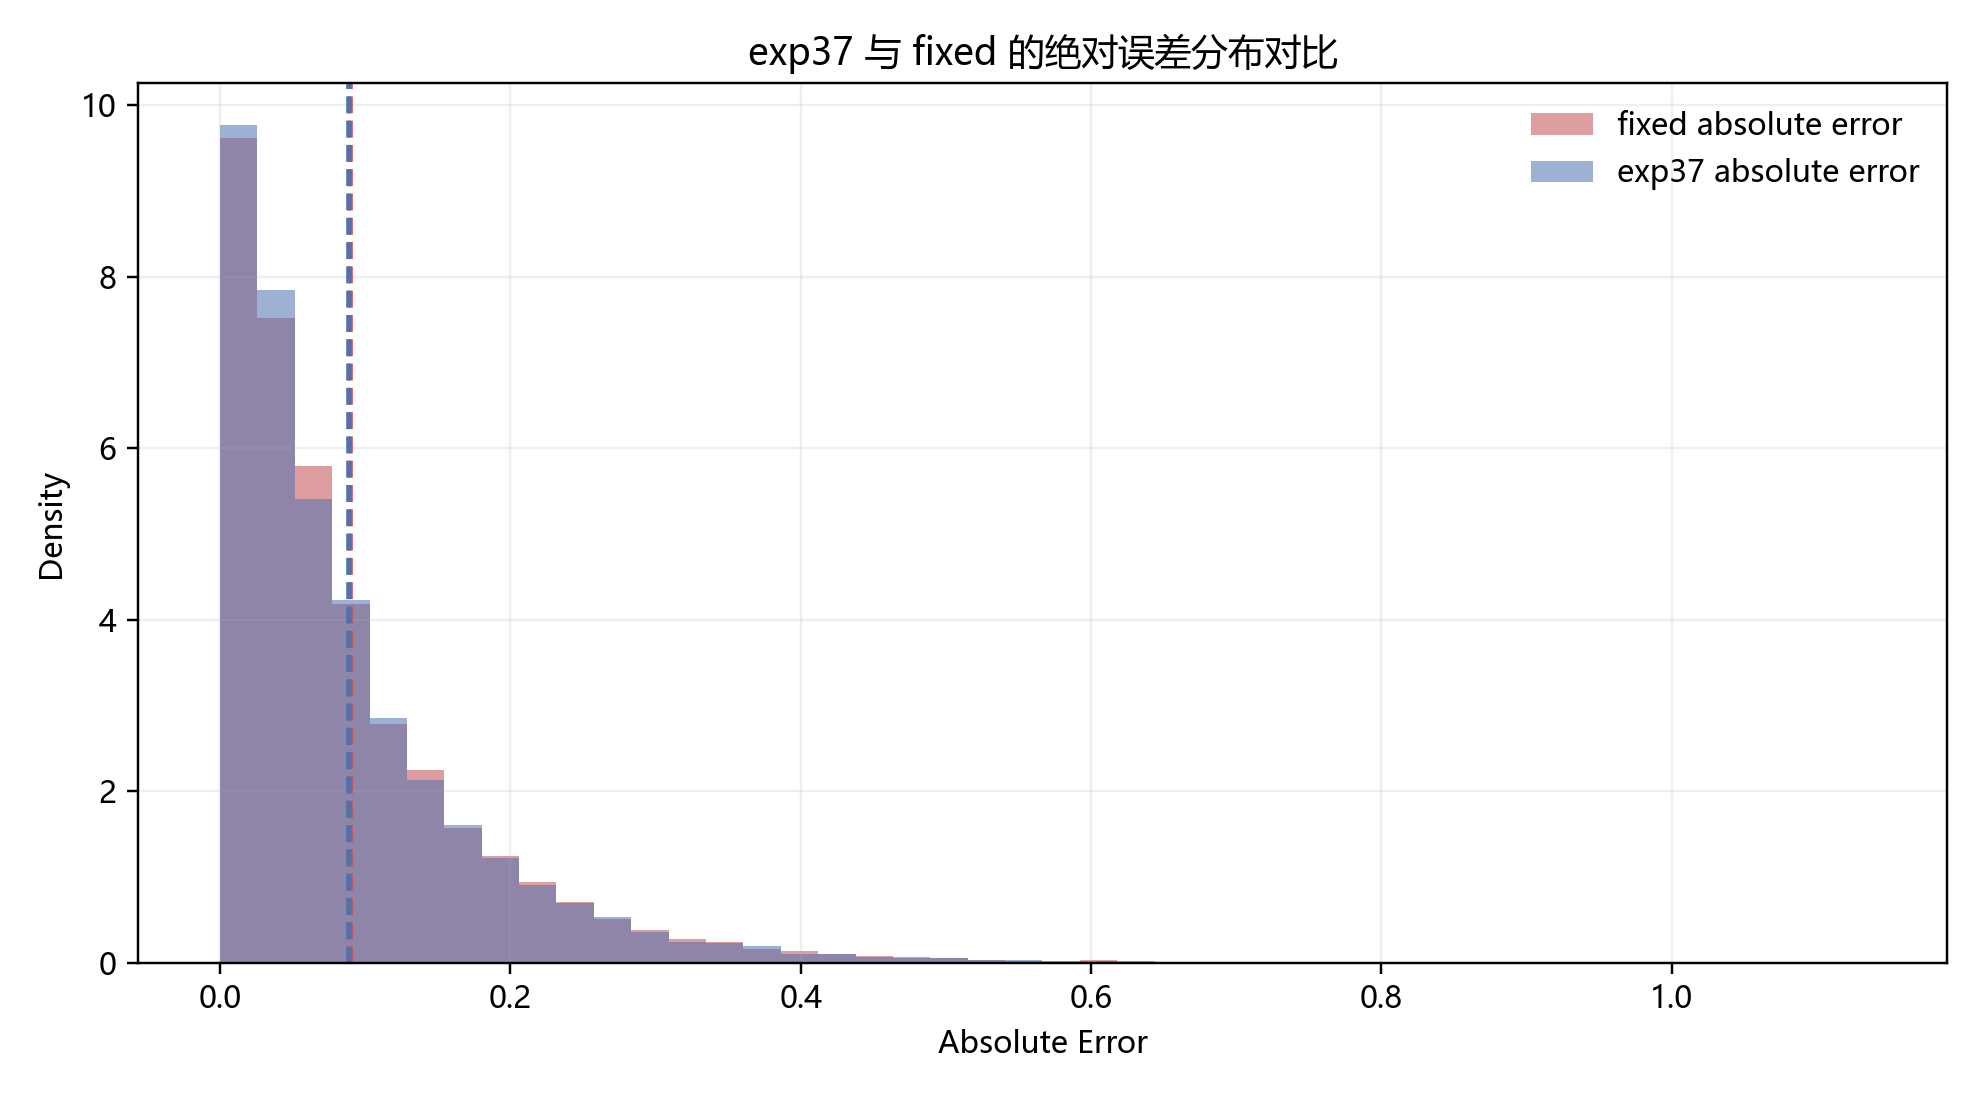
\includegraphics[width=0.92\linewidth]{figures/exp37_error_distribution.png}
\caption{exp37 最优方案与 fixed 基线的误差分布对比。}
\label{fig:error}
\end{figure}

图 \ref{fig:error} 从误差分布角度说明这种提升并非来自极少数异常点，而是整体误差分布向更小区间收缩。换句话说，量子弱融合的收益不是偶然命中少量样本，而是在更大范围内压缩了误差尾部。就定量结果而言，绝对误差的 $90\%$ 分位数由 `fixed` 的 $0.2055$ 下降到最优量子方案的 $0.2030$，下降约 $1.20\%$；$95\%$ 分位数由 $0.2704$ 下降到 $0.2674$，下降约 $1.12\%$。

更重要的是，图 \ref{fig:error} 中大误差区间的频数下降更明显，这意味着量子弱融合的主要贡献不只是继续优化已经较好的样本，而是在若干原本更难处理的时间步上降低了极端偏差。对于数据同化任务而言，这类“尾部风险”的收缩往往比平均误差的微小变化更有意义，因为它直接关系到分析场在动力系统演化中的稳定性。

\begin{figure}[htbp]
\centering
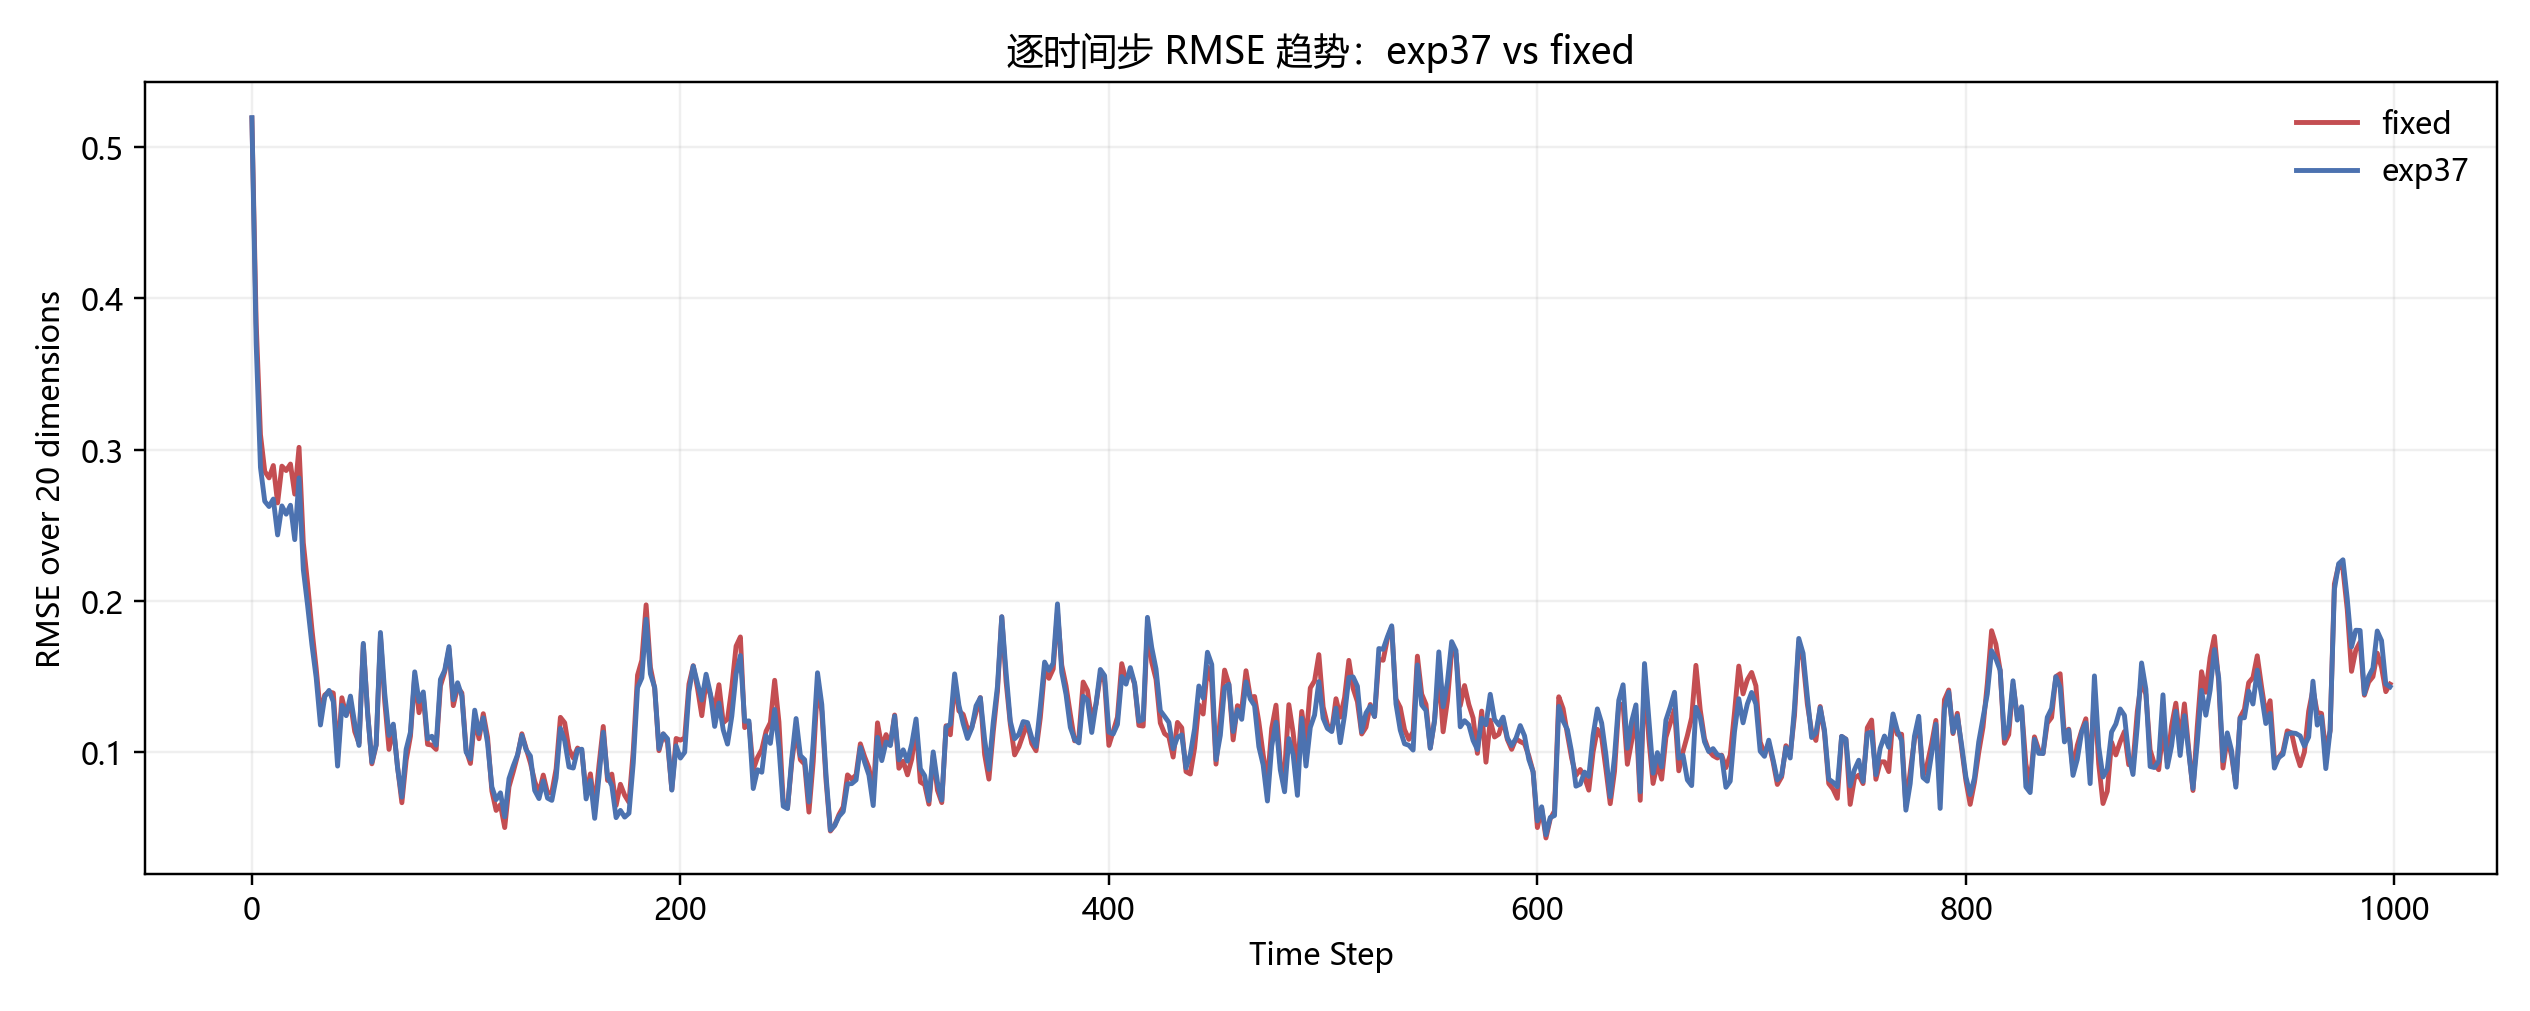
\includegraphics[width=0.92\linewidth]{figures/exp37_time_rmse_trend.png}
\caption{exp37 与 fixed 的逐时间步 RMSE 趋势对比。}
\label{fig:trend}
\end{figure}

图 \ref{fig:trend} 展示了逐时间步上的 RMSE 变化情况。可以看到，量子弱融合并不是只在极个别时间片上优于 fixed，而是在较长时间段内保持相对稳定的优势，这说明该方法对动力系统演化过程具有一定持续适应性。进一步统计可知，在有定义的 $999$ 个时间步中，最优量子方案在 $250$ 个时间步上优于 `fixed`，在 $250$ 个时间步上劣于 `fixed`，其余时间步二者几乎持平。也就是说，最终总体 RMSE 的提升并不是来自“更多时间步取胜”，而是来自“关键时间步上的改善幅度更大”，这一点与弱局地修正的设计目标是一致的。

如果一种方法只在少量时间点上偶然优于基线，那么它更可能是在“碰巧对齐”某些局部模式，而不是真正学到了可迁移的结构信息。图 \ref{fig:trend} 恰恰说明本文方法不是这种情况：它在多个连续时间段内都维持了较平稳的误差优势，因此更能支撑“量子结构信息提供了稳定的局地修正线索”这一判断。

\begin{figure}[htbp]
\centering
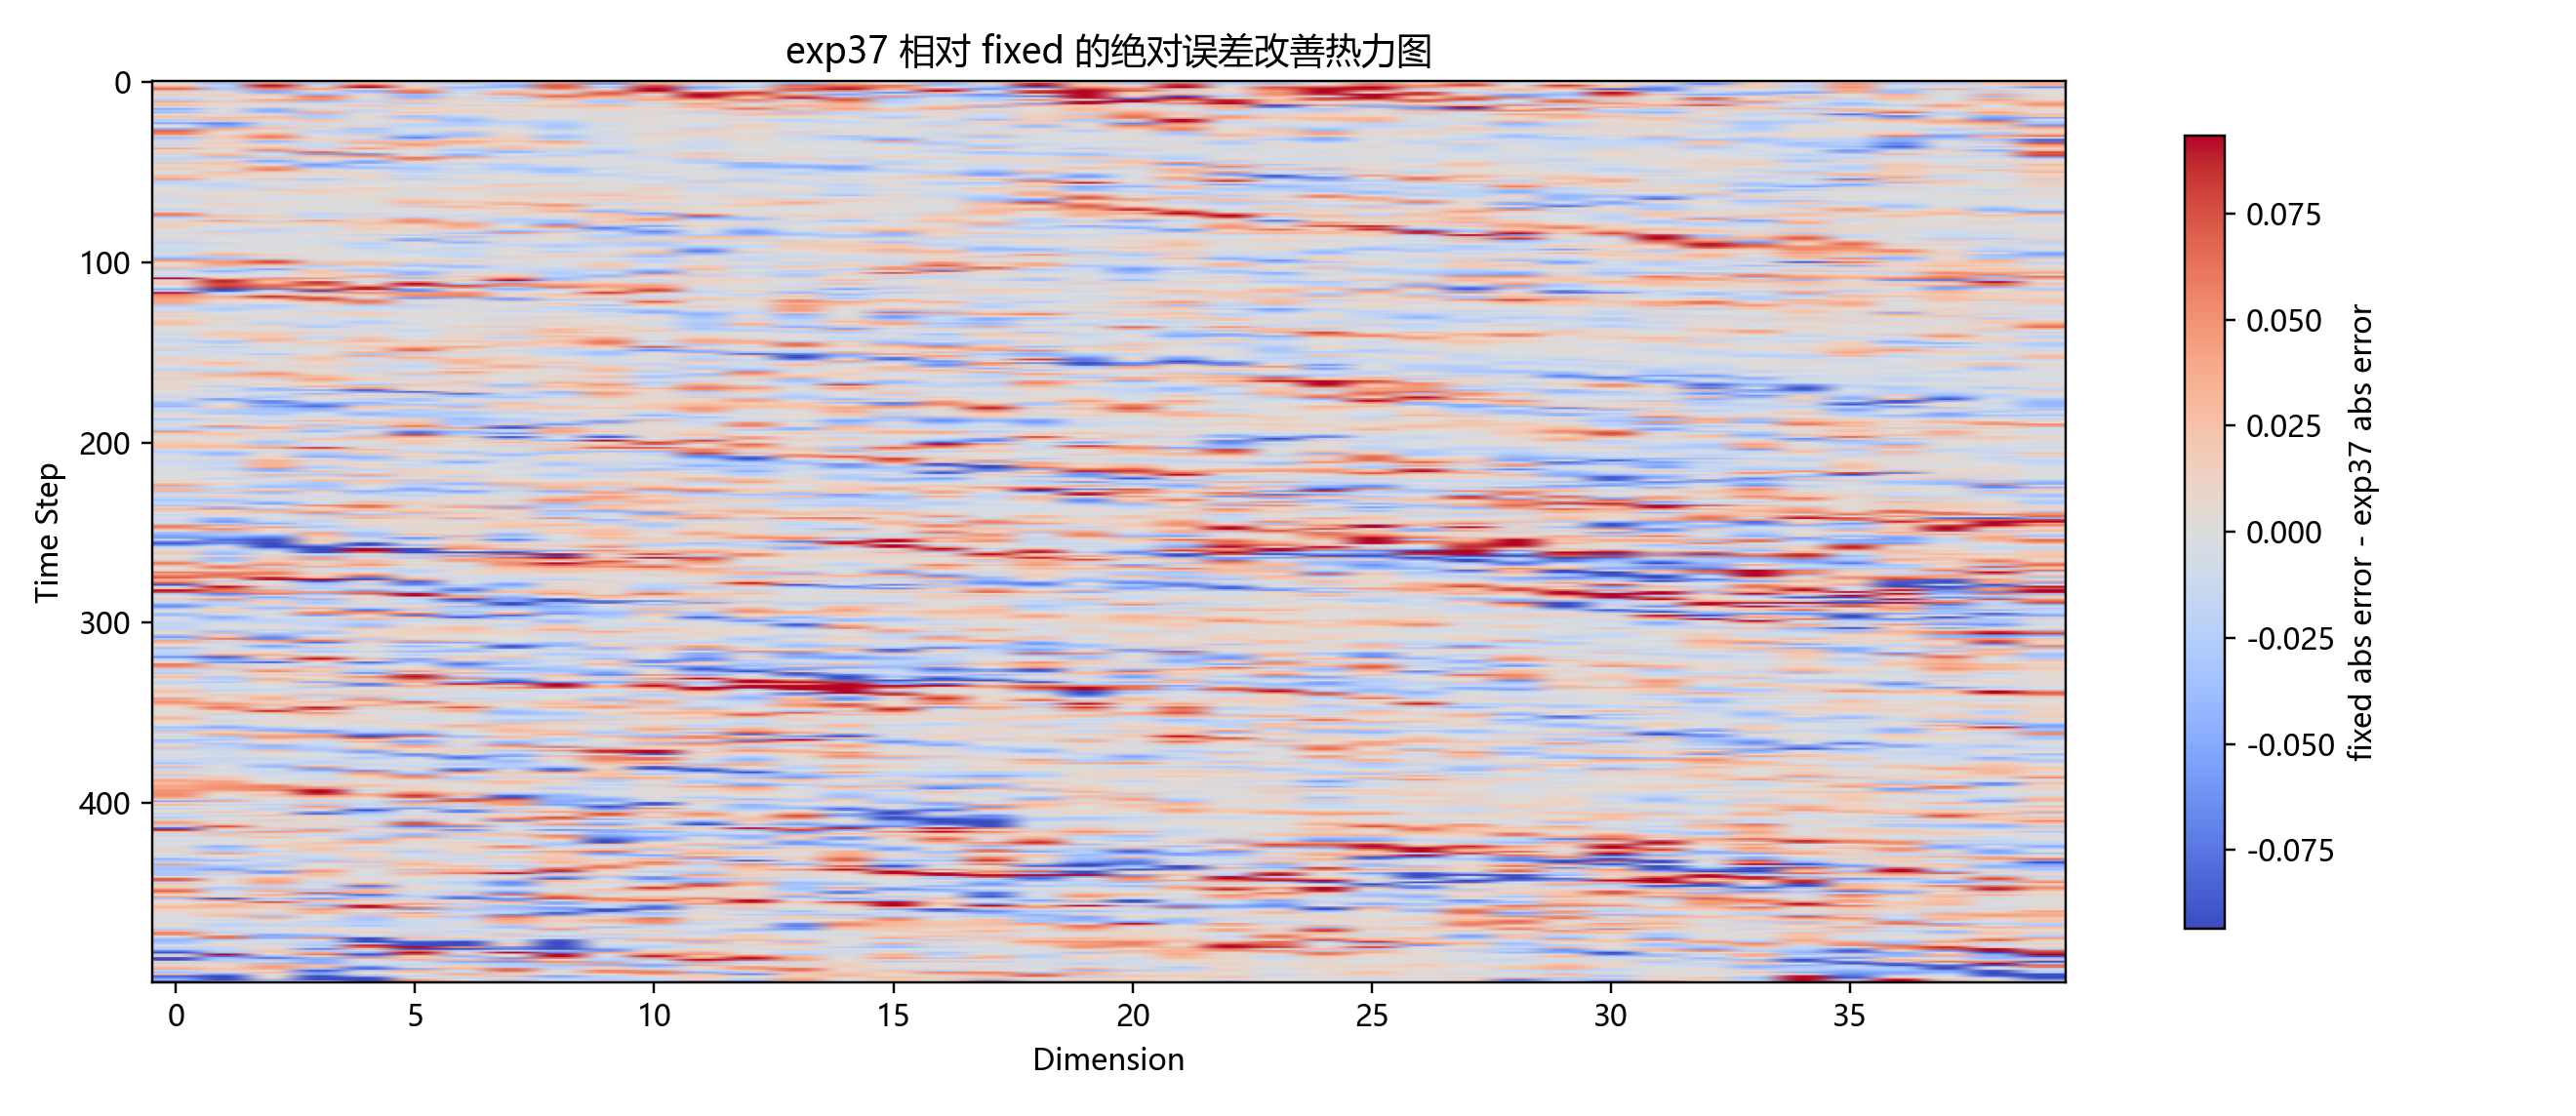
\includegraphics[width=0.92\linewidth]{figures/exp37_error_improvement_heatmap.png}
\caption{exp37 相对 fixed 的逐时间步、逐维度误差改善热力图。}
\label{fig:heatmap}
\end{figure}

图 \ref{fig:heatmap} 则进一步给出了改善发生的位置。该图说明收益并不是均匀分布的，而是在部分时间步和部分维度上更明显。这与本文的局地窗口建模假设是一致的：量子结构信号主要影响局地几何关系，因此其改进也首先体现在局部区域，而不是全局平均地同时提升。

这张热力图的意义还在于，它把“为什么不是全局统一提升”解释清楚了。本文的方法本来就不是全局替代型方法，而是围绕局地窗口构造量子相似度，因此它的收益理应表现为某些局部维度、某些局部时间段的更明显改善。换句话说，图 \ref{fig:heatmap} 不是在暴露方法的局限，反而是在证明方法行为与设计假设一致。

\begin{figure}[htbp]
\centering
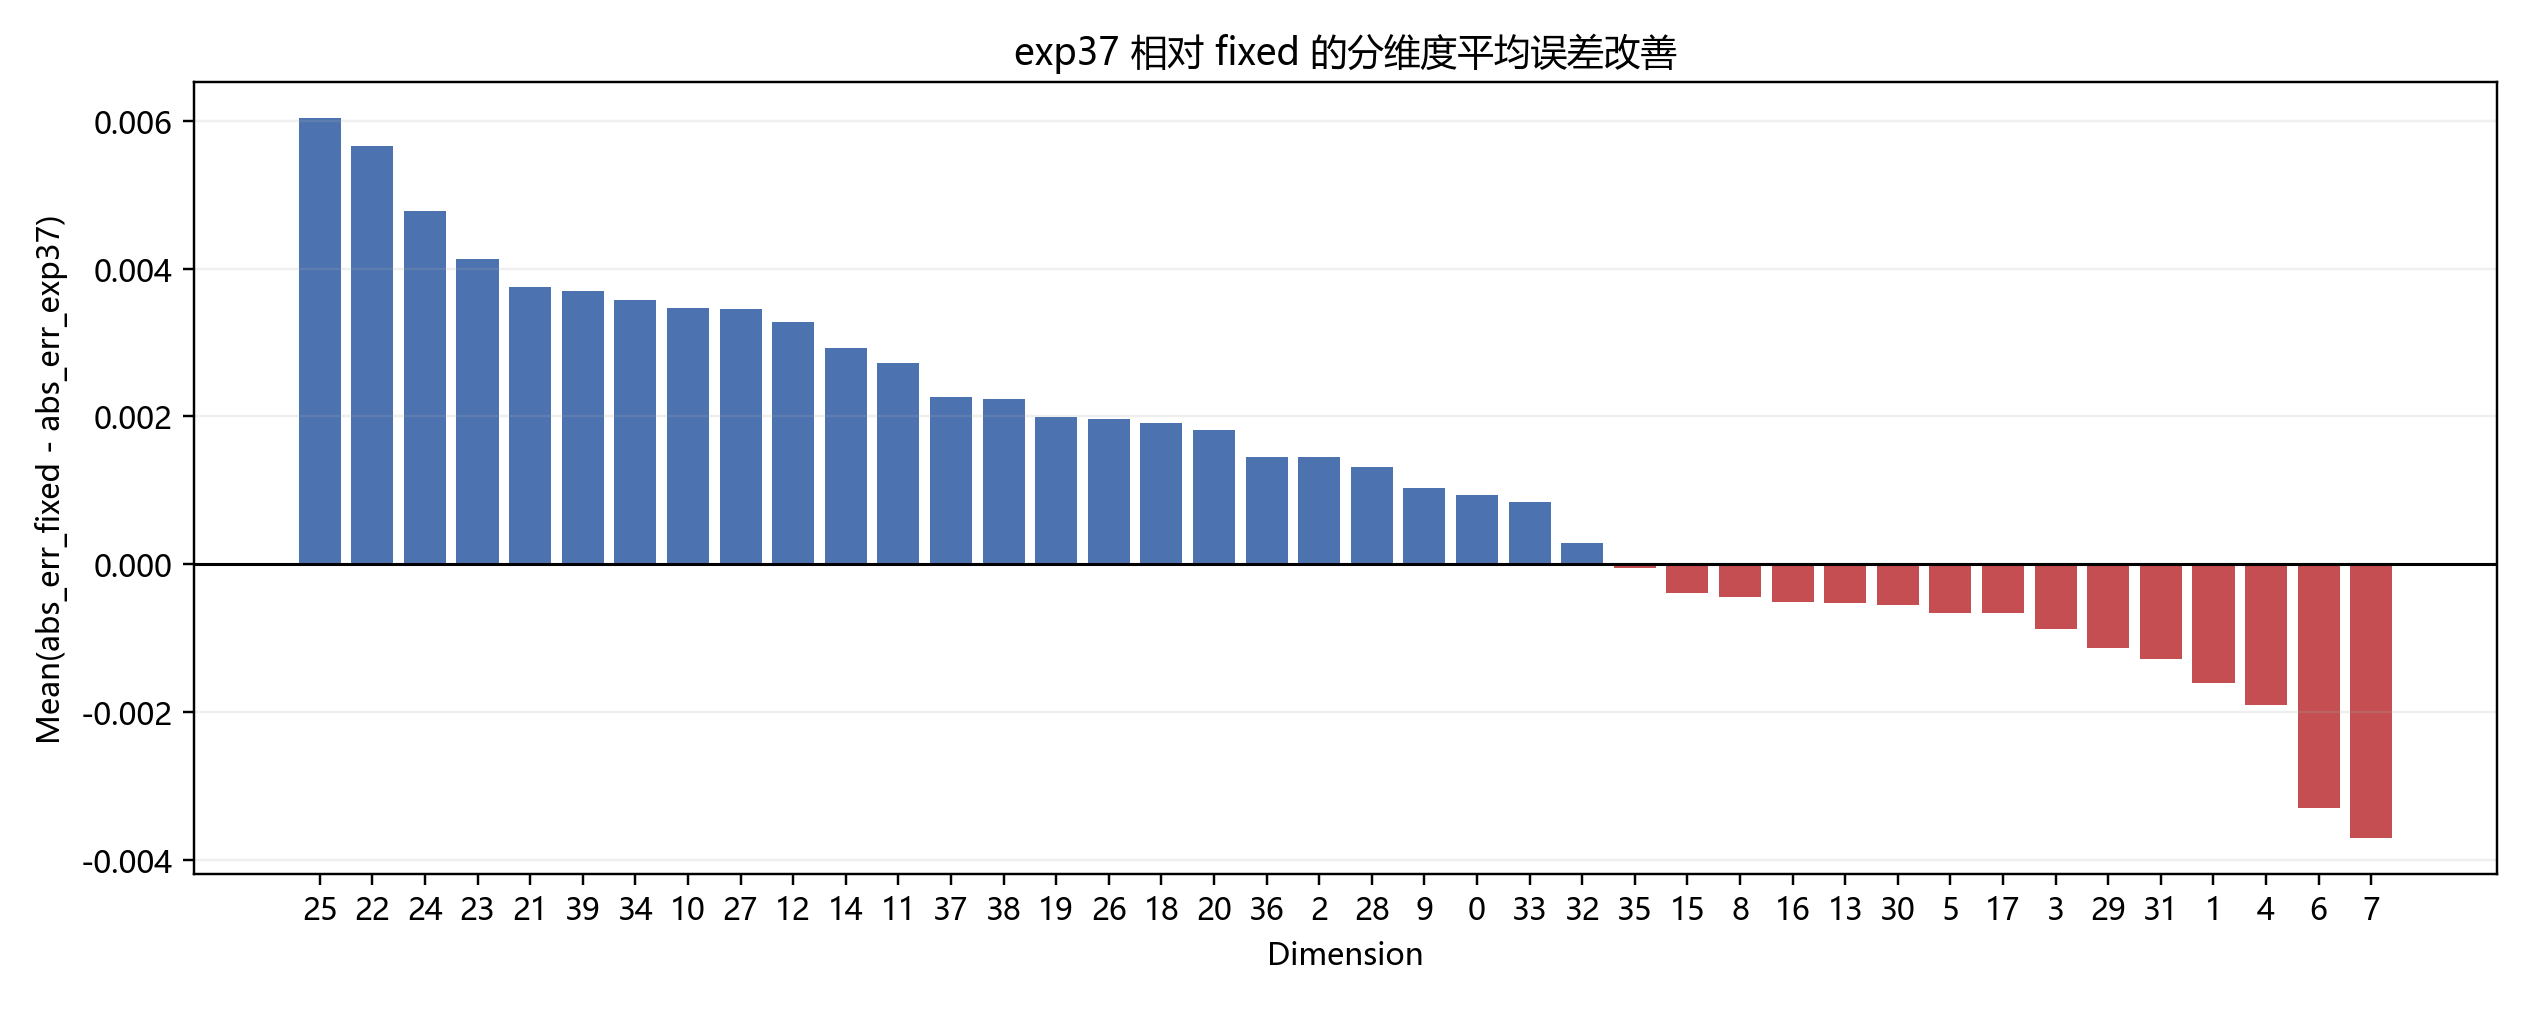
\includegraphics[width=0.92\linewidth]{figures/exp37_dimension_gain.png}
\caption{exp37 相对 fixed 的分维度平均绝对误差改善。}
\label{fig:dim-gain}
\end{figure}

图 \ref{fig:dim-gain} 把热力图中的局部改善进一步压缩为维度层面的统计量。可以看到，收益并非平均分配在所有状态维度上，而是有些维度改善更明显，有些维度变化较小。定量上，$40$ 个维度中有 $25$ 个维度的平均绝对误差优于 `fixed`。改善最明显的五个维度是 $25,22,24,23,21$，其维度平均绝对误差分别下降约 $0.0060,0.0057,0.0048,0.0041,0.0038$。这一现象再次说明，量子弱融合并不是简单给所有维度统一减小误差，而是在更容易出现局地模式错配的维度上提供了额外帮助。

\begin{figure}[htbp]
\centering
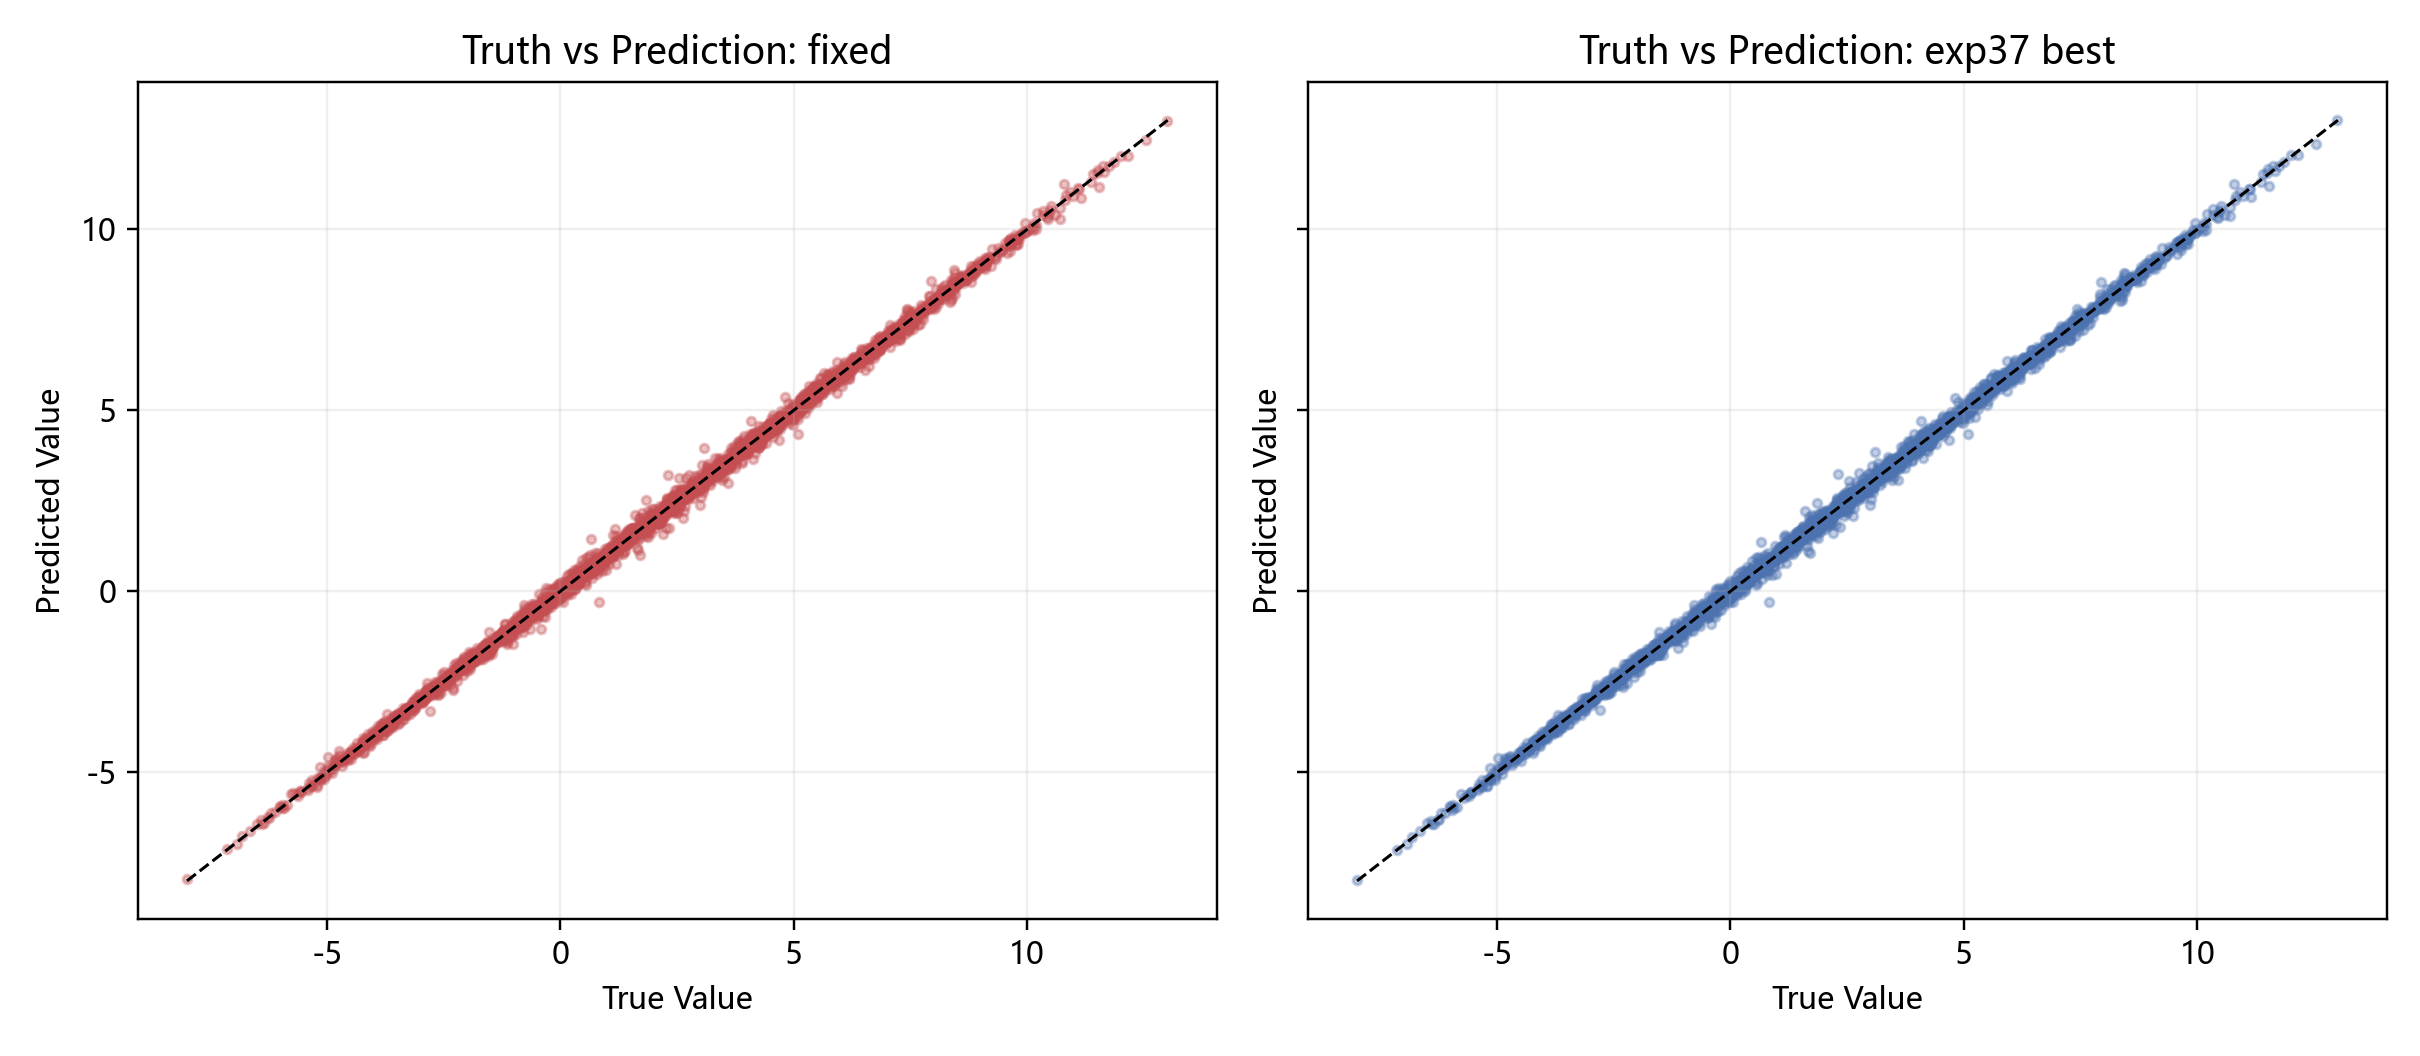
\includegraphics[width=0.92\linewidth]{figures/exp37_prediction_scatter.png}
\caption{fixed 与 exp37 最优方案的 truth-prediction 散点对比。}
\label{fig:scatter}
\end{figure}

图 \ref{fig:scatter} 从预测值与真实值的散点贴合关系出发，进一步展示了最优 exp37 方案的整体重建质量。若散点更多沿对角线分布，说明分析结果更接近真实状态。与 fixed 相比，exp37 的散点云更集中、更贴近理想对角线，说明其改进不仅体现在总体误差指标上，也体现在状态重建的几何一致性上。

\begin{figure}[htbp]
\centering
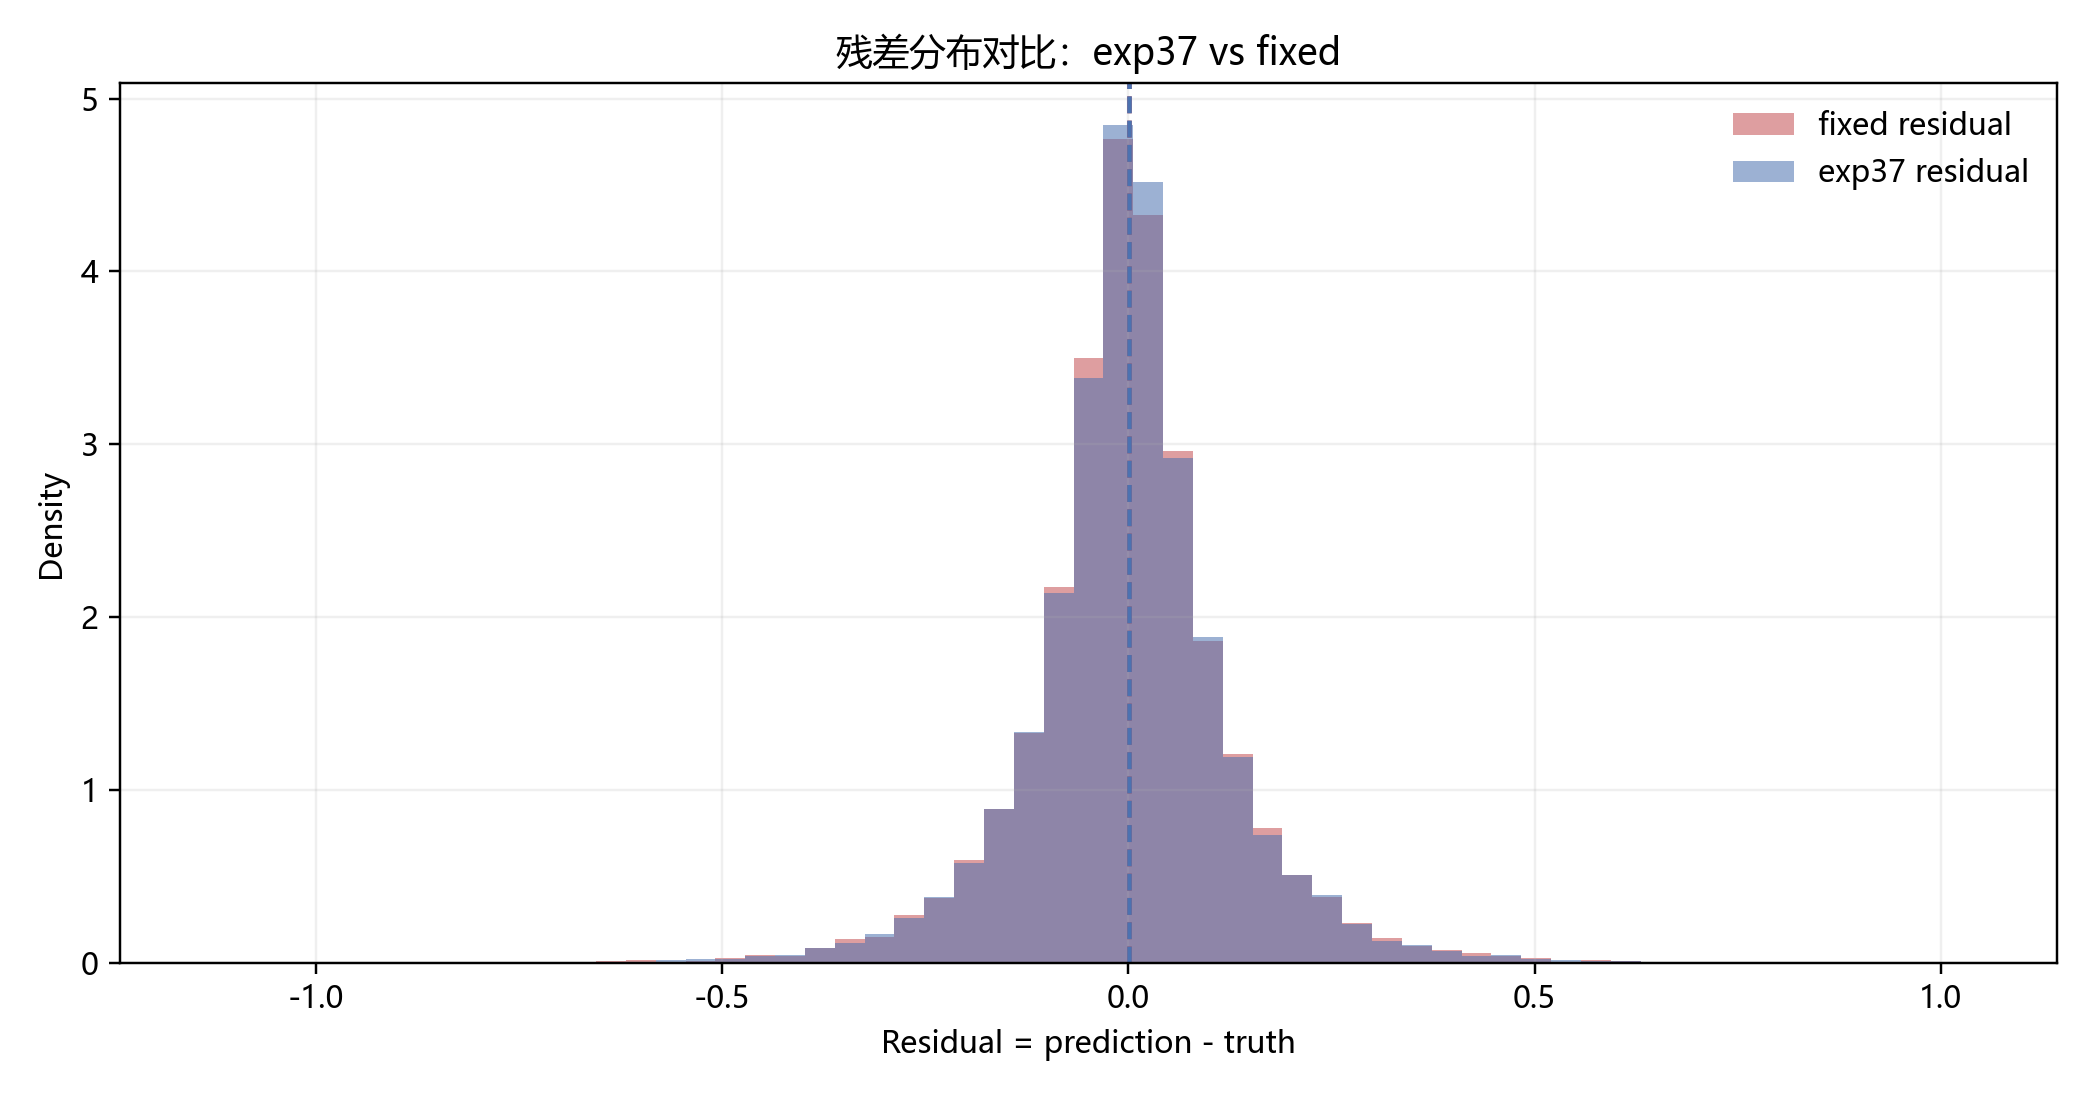
\includegraphics[width=0.92\linewidth]{figures/exp37_residual_distribution.png}
\caption{exp37 与 fixed 的残差分布对比。}
\label{fig:residual}
\end{figure}

图 \ref{fig:residual} 给出了残差分布的进一步证据。可以看到，exp37 的残差中心更接近零点，分布宽度也更窄，这说明该方法不仅降低了绝对误差，也在一定程度上减少了系统性偏差和大范围波动。定量上，残差均值由 `fixed` 的 $7.08\times 10^{-4}$ 收缩到 $5.59\times 10^{-4}$，残差标准差由 $0.12873$ 收缩到 $0.12698$。对评估一个同化方法是否真正稳定来说，这比单独看 RMSE 更有解释力。

\begin{figure}[htbp]
\centering
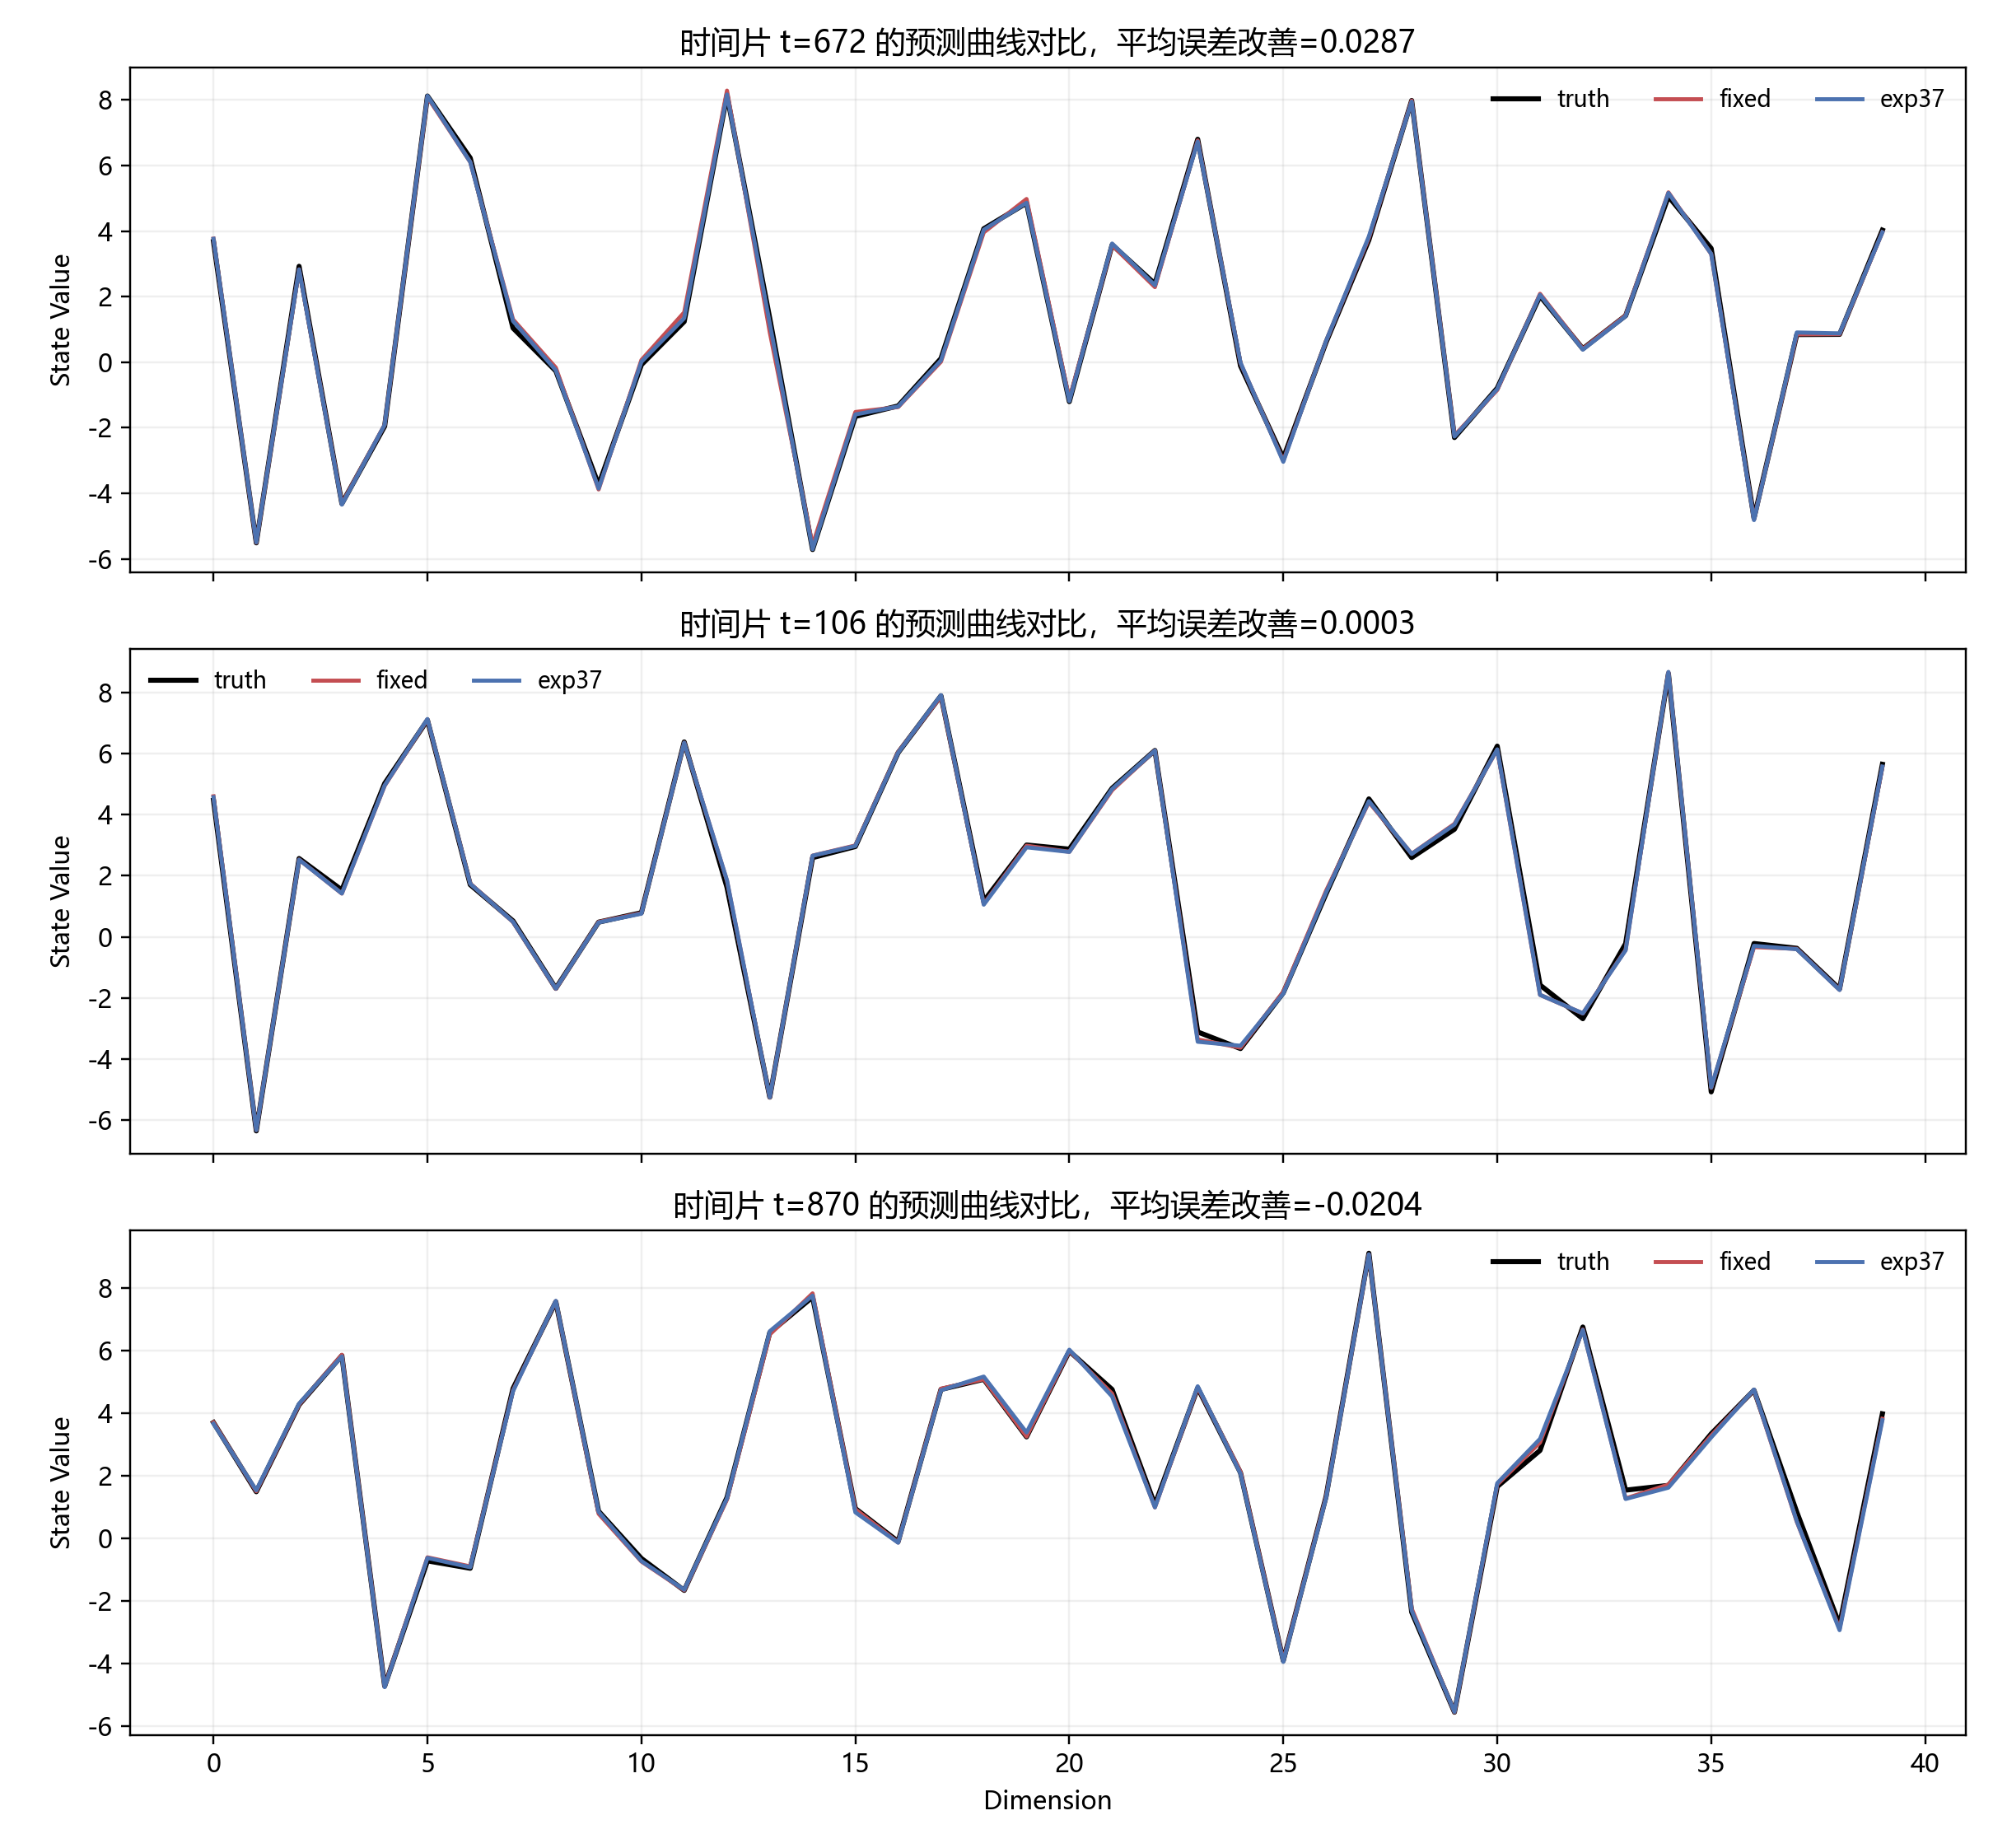
\includegraphics[width=0.92\linewidth]{figures/exp37_case_slices.png}
\caption{代表性时间片上 truth、fixed 与 exp37 的状态切片对比。}
\label{fig:slices}
\end{figure}

最后，图 \ref{fig:slices} 给出了最直观的状态切片对比。相比 fixed，exp37 在若干代表性时间片上对峰值、谷值以及局地转折位置的跟踪更贴近真实曲线。这说明量子弱融合带来的并不是抽象指标上的微小变化，而是对局地状态形状恢复能力的实际增强。对于论文报告而言，这类图尤为重要，因为它把“量子结构信息改善了局地几何重建”这一核心故事，转化成了可直接观察的证据。

\begin{figure}[htbp]
\centering
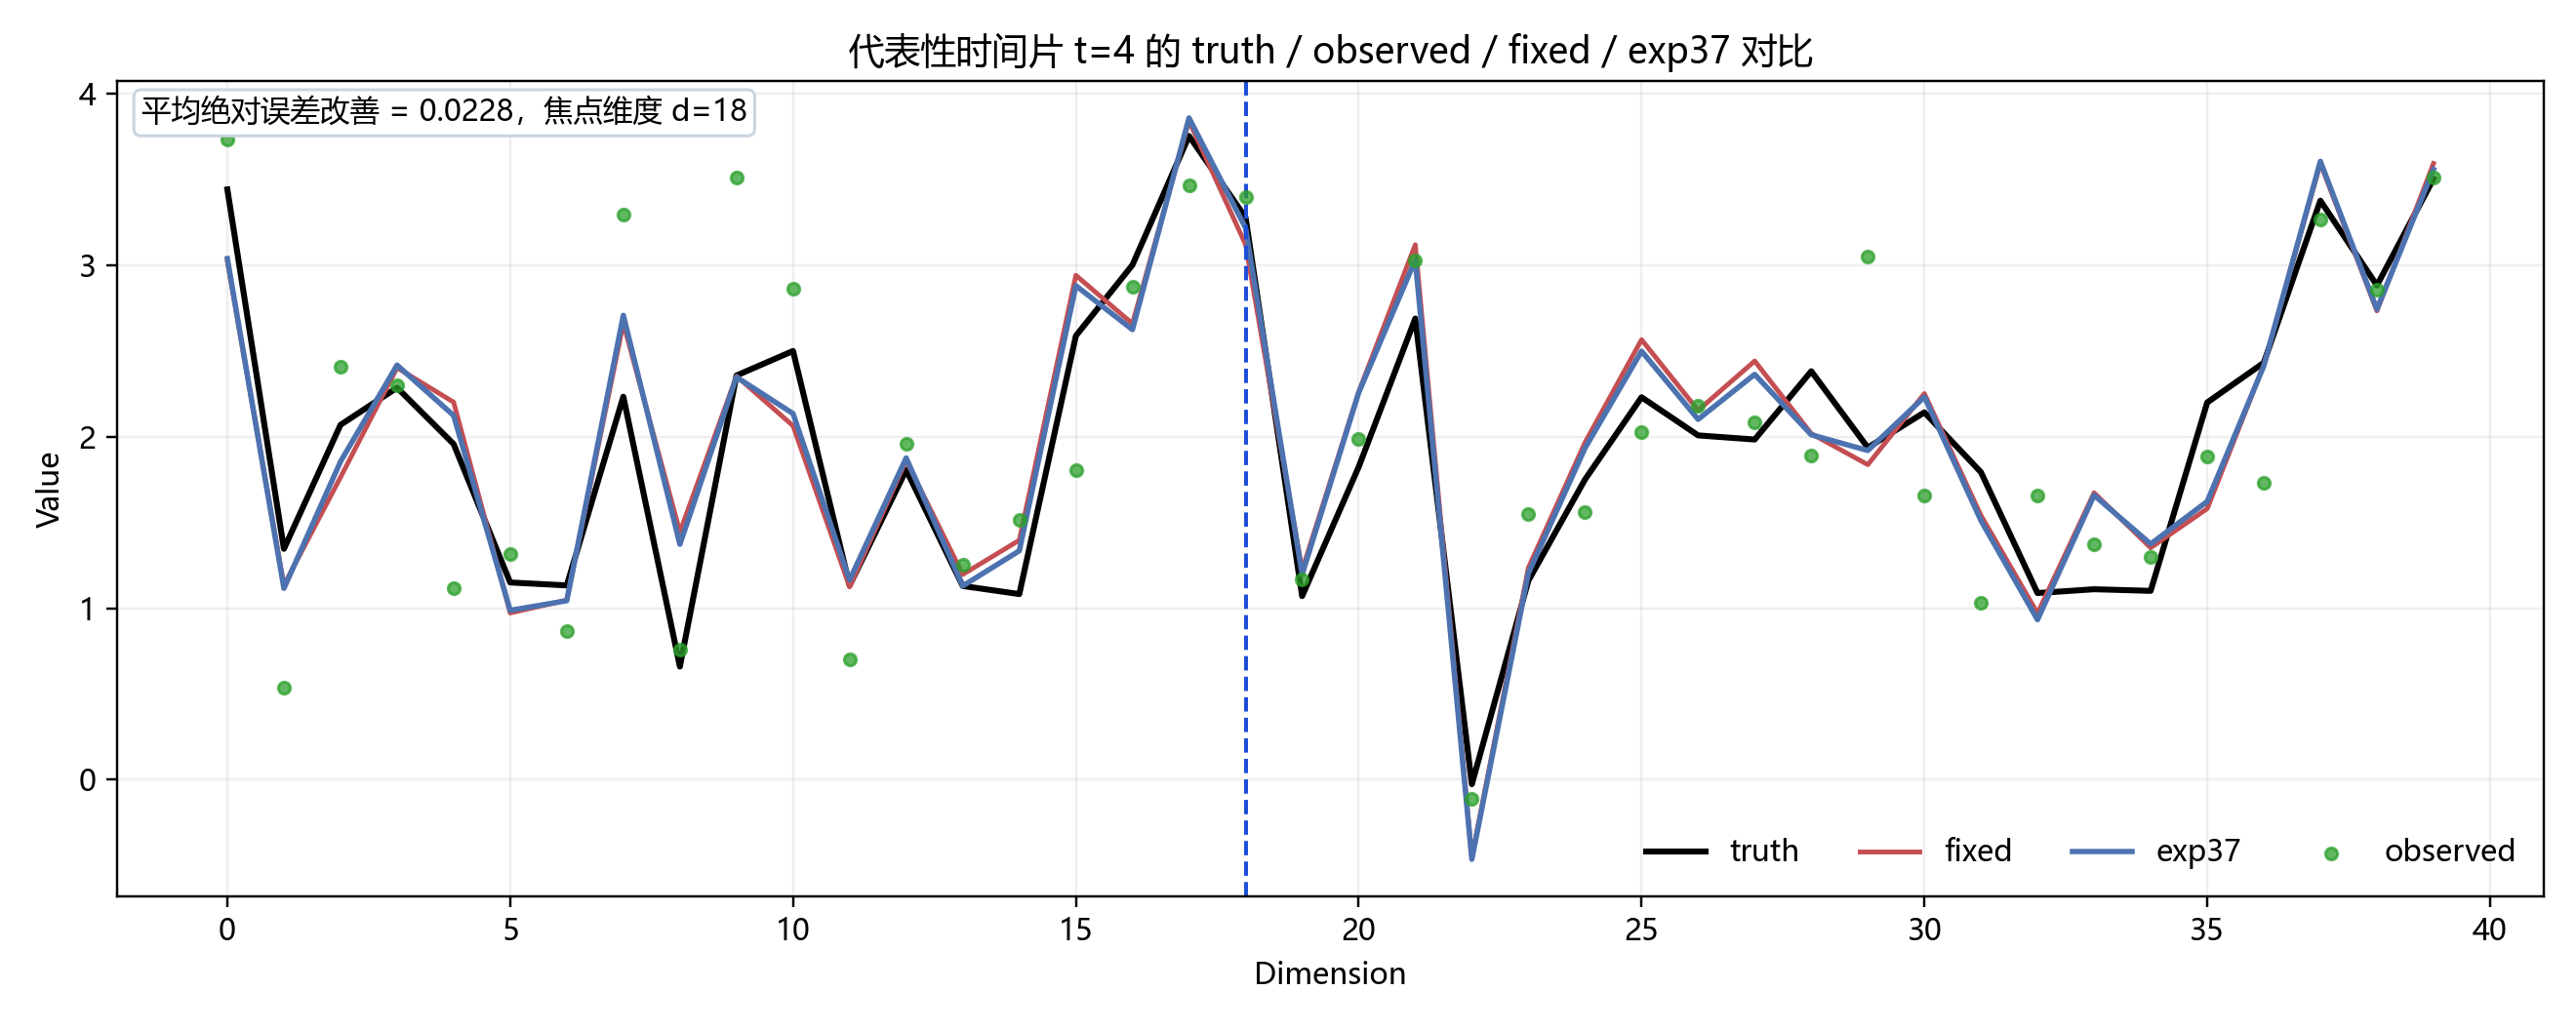
\includegraphics[width=0.92\linewidth]{figures/exp37_observed_truth_fixed_best_slice.png}
\caption{代表性高收益时间片上 observed、truth、fixed 与 exp37 的状态切片对比。}
\label{fig:obs-slice}
\end{figure}

图 \ref{fig:obs-slice} 则把观测值也引入了比较。这样做的好处是，可以区分“更贴近观测”和“更贴近真实状态”这两件事。在带噪观测条件下，一个方法如果只是过度追随观测，不一定意味着同化更好；而图 \ref{fig:obs-slice} 显示，exp37 在关键时间片上既没有简单复制带噪观测，也没有停留在 fixed 的平均化趋势上，而是在二者之间更好地恢复了真实曲线形态。定量上，该代表性高收益时间片对应 $t=672$，此时 `fixed` 的切片 RMSE 为 $0.1229$，最优量子方案为 $0.0781$，单时间片下降约 $36.5\%$。这一图直接体现了数据同化任务中最重要的能力，即在模型和观测之间找到更合理的平衡点。

\section{创新点描述（与现有量子算法或经典算法的差异与优势）}
若从已有路线出发，本文的创新点应当被理解为“相对创新”而非绝对首创。与经典 LETKF/局地加权路线相比，本文额外引入了可解释的量子相似度结构\cite{hunt2007letkf}；与量子核或量子特征映射路线相比，本文没有停留在相似度矩阵展示，而是把该相似度嵌入局地同化权重\cite{yin2025photonicqkernel,saez2025qkernel,altmann2025qgk}；与量子数据同化或算子代数路线相比，本文没有试图让量子模块整体替代状态估计，而是只让其进入 LETKF 的局地结构层\cite{kotsuki2024qda,giannakis2022operator}。基于这种定位，本文的主要创新点可概括为以下三方面：
\begin{itemize}
\item \textbf{作用位点创新}：相对于仅把量子模块用于超参数搜索的做法，本文把量子信息嵌入到 LETKF 的局地权重与弱方向修正中，使量子模块进入同化公式内部而不是停留在外层；
\item \textbf{表示层创新}：相对于只报告量子核矩阵或相似度矩阵的做法，本文利用局地窗口量子特征映射构造状态--观测相似度，并将其明确解释为局地几何结构编码器；
\item \textbf{融合机制创新}：相对于直接结构化加权或强替代更新的做法，本文采用“距离先验 + 量子相似度”的弱融合方式，并通过小幅 $J$ 修正限制量子信号强度，使量子增强与经典稳定性兼容。
\end{itemize}

如果只把上述三点列成条目，仍然不足以体现本文方法的真正创新性。本文的价值不在于单独提出某一个新公式，而在于把“量子信息如何进入同化器”这一问题拆成了可分析的几个层次，并在每个层次上给出对应的结构解释。换句话说，创新不仅体现在结果更优，也体现在方法的可解释性更完整。

\begin{figure}[htbp]
\centering
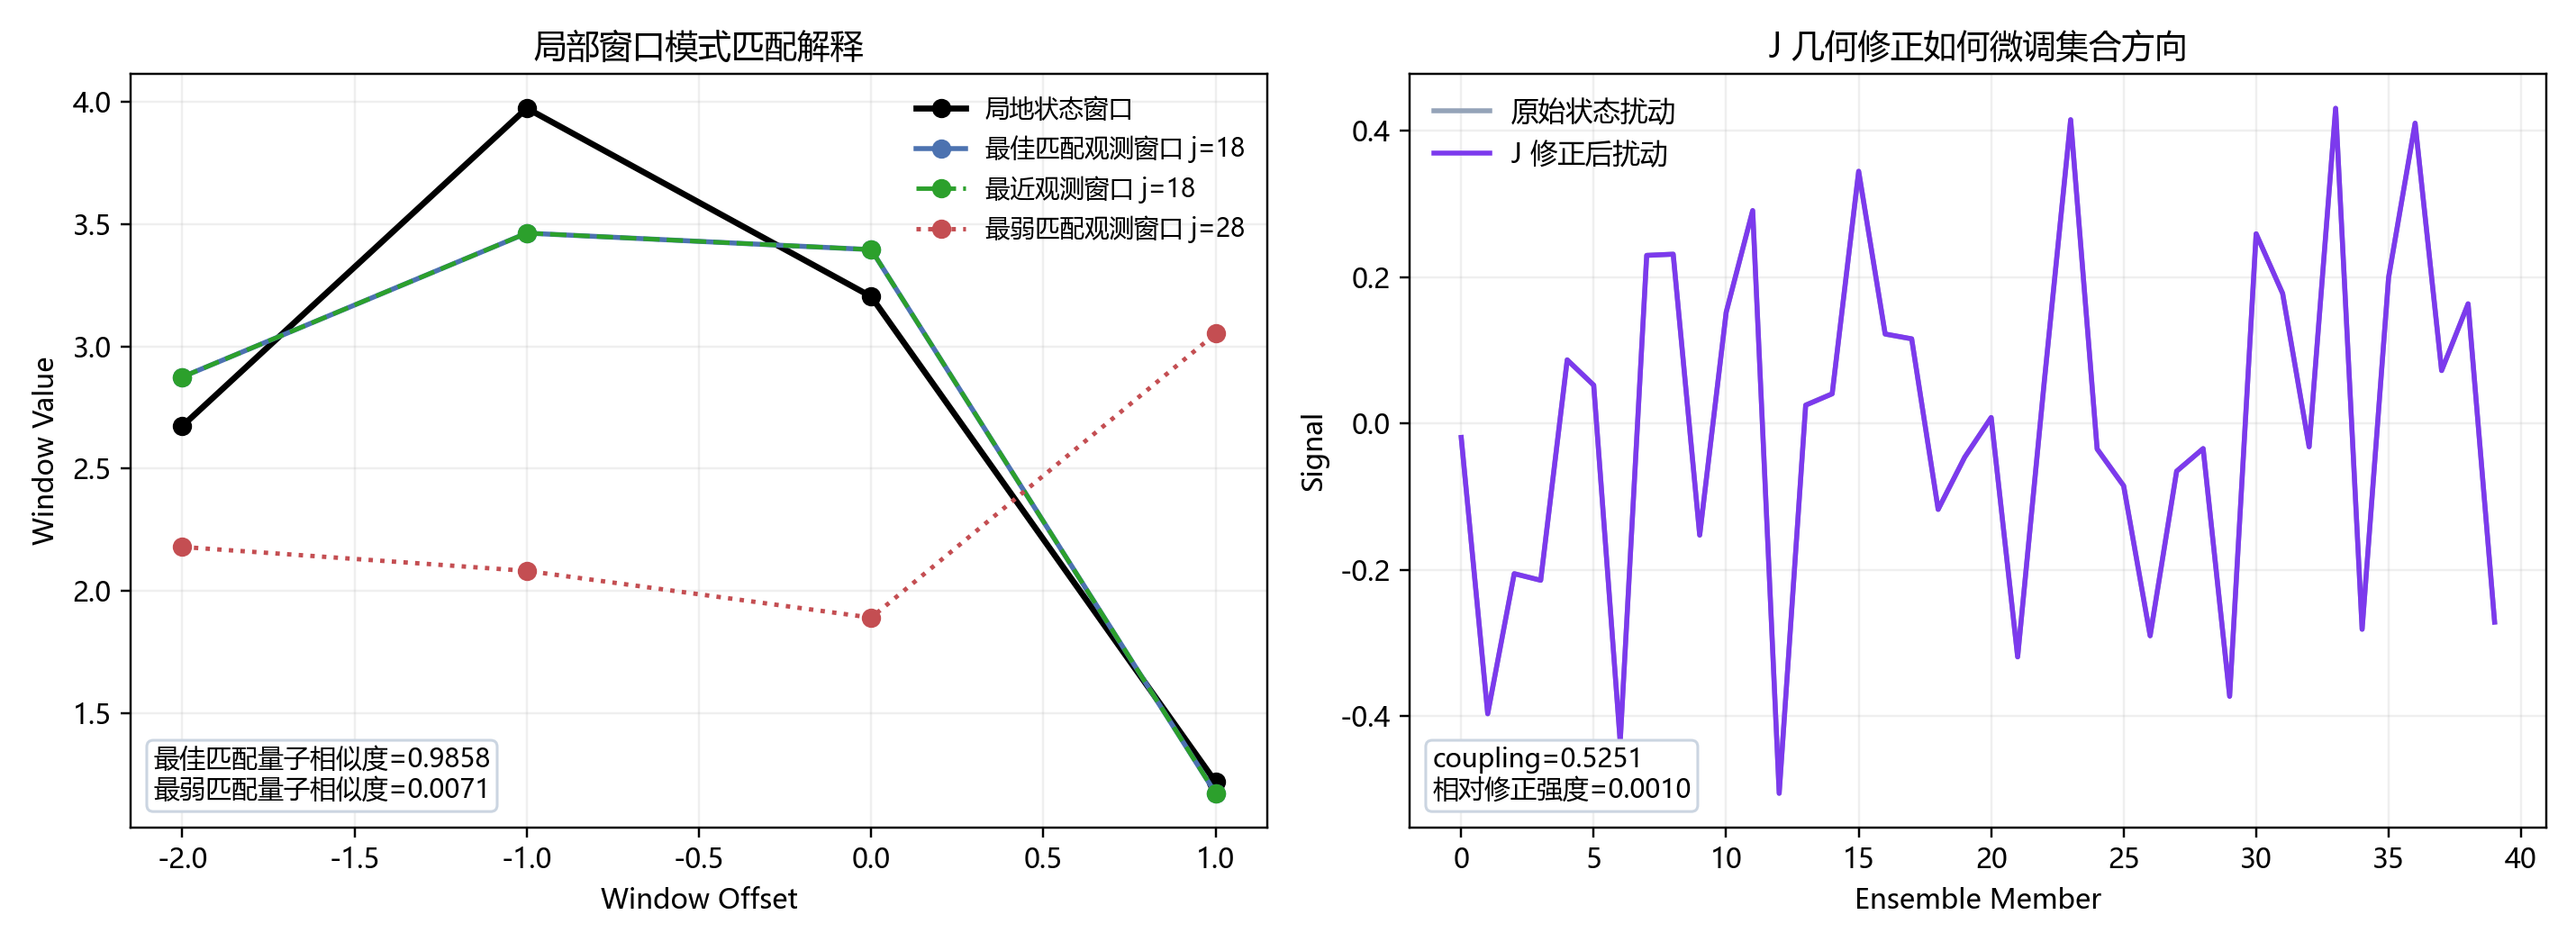
\includegraphics[width=0.92\linewidth]{figures/exp37_local_window_explanation.png}
\caption{代表性局地窗口下的状态模式、观测模式与弱 $J$ 修正示意。}
\label{fig:local}
\end{figure}

图 \ref{fig:local} 是本文创新点最直接的可视化证据。它说明量子模块并不是抽象地输出一个权重系数，而是在局地窗口内刻画状态模式与观测模式的匹配关系，并据此对集合方向做小幅修正。因此，本文最重要的创新不在于“量子线路更复杂”，而在于给出了一个可追踪的信号流：局地窗口 $\rightarrow$ 相似度 $\rightarrow$ 局地模式 $\rightarrow$ 弱修正。

进一步看，图中的局地模式匹配关系说明了一个重要事实：量子模块的价值不在于生成一个全局最优参数，而在于识别哪些局地观测更值得被当前状态窗口强调。也正因为这种匹配关系是局地的、几何的，所以弱 $J$ 修正必须保持小幅，否则就会把原本有价值的局地提示放大成不稳定的全局扰动。

这也是本文“可解释性”最核心的一层。传统上，量子模块很容易被理解为一个难以分析的黑箱相似度生成器，但图 \ref{fig:local} 说明它其实有非常明确的角色分工：一部分作用于识别局地窗口之间的结构相近性，另一部分作用于判断集合扰动方向是否应被轻微修正。也就是说，量子模块输出的不是不可追踪的神秘特征，而是可以通过局地窗口、模式匹配和方向变化三步解释清楚的结构信号。

\begin{figure}[htbp]
\centering
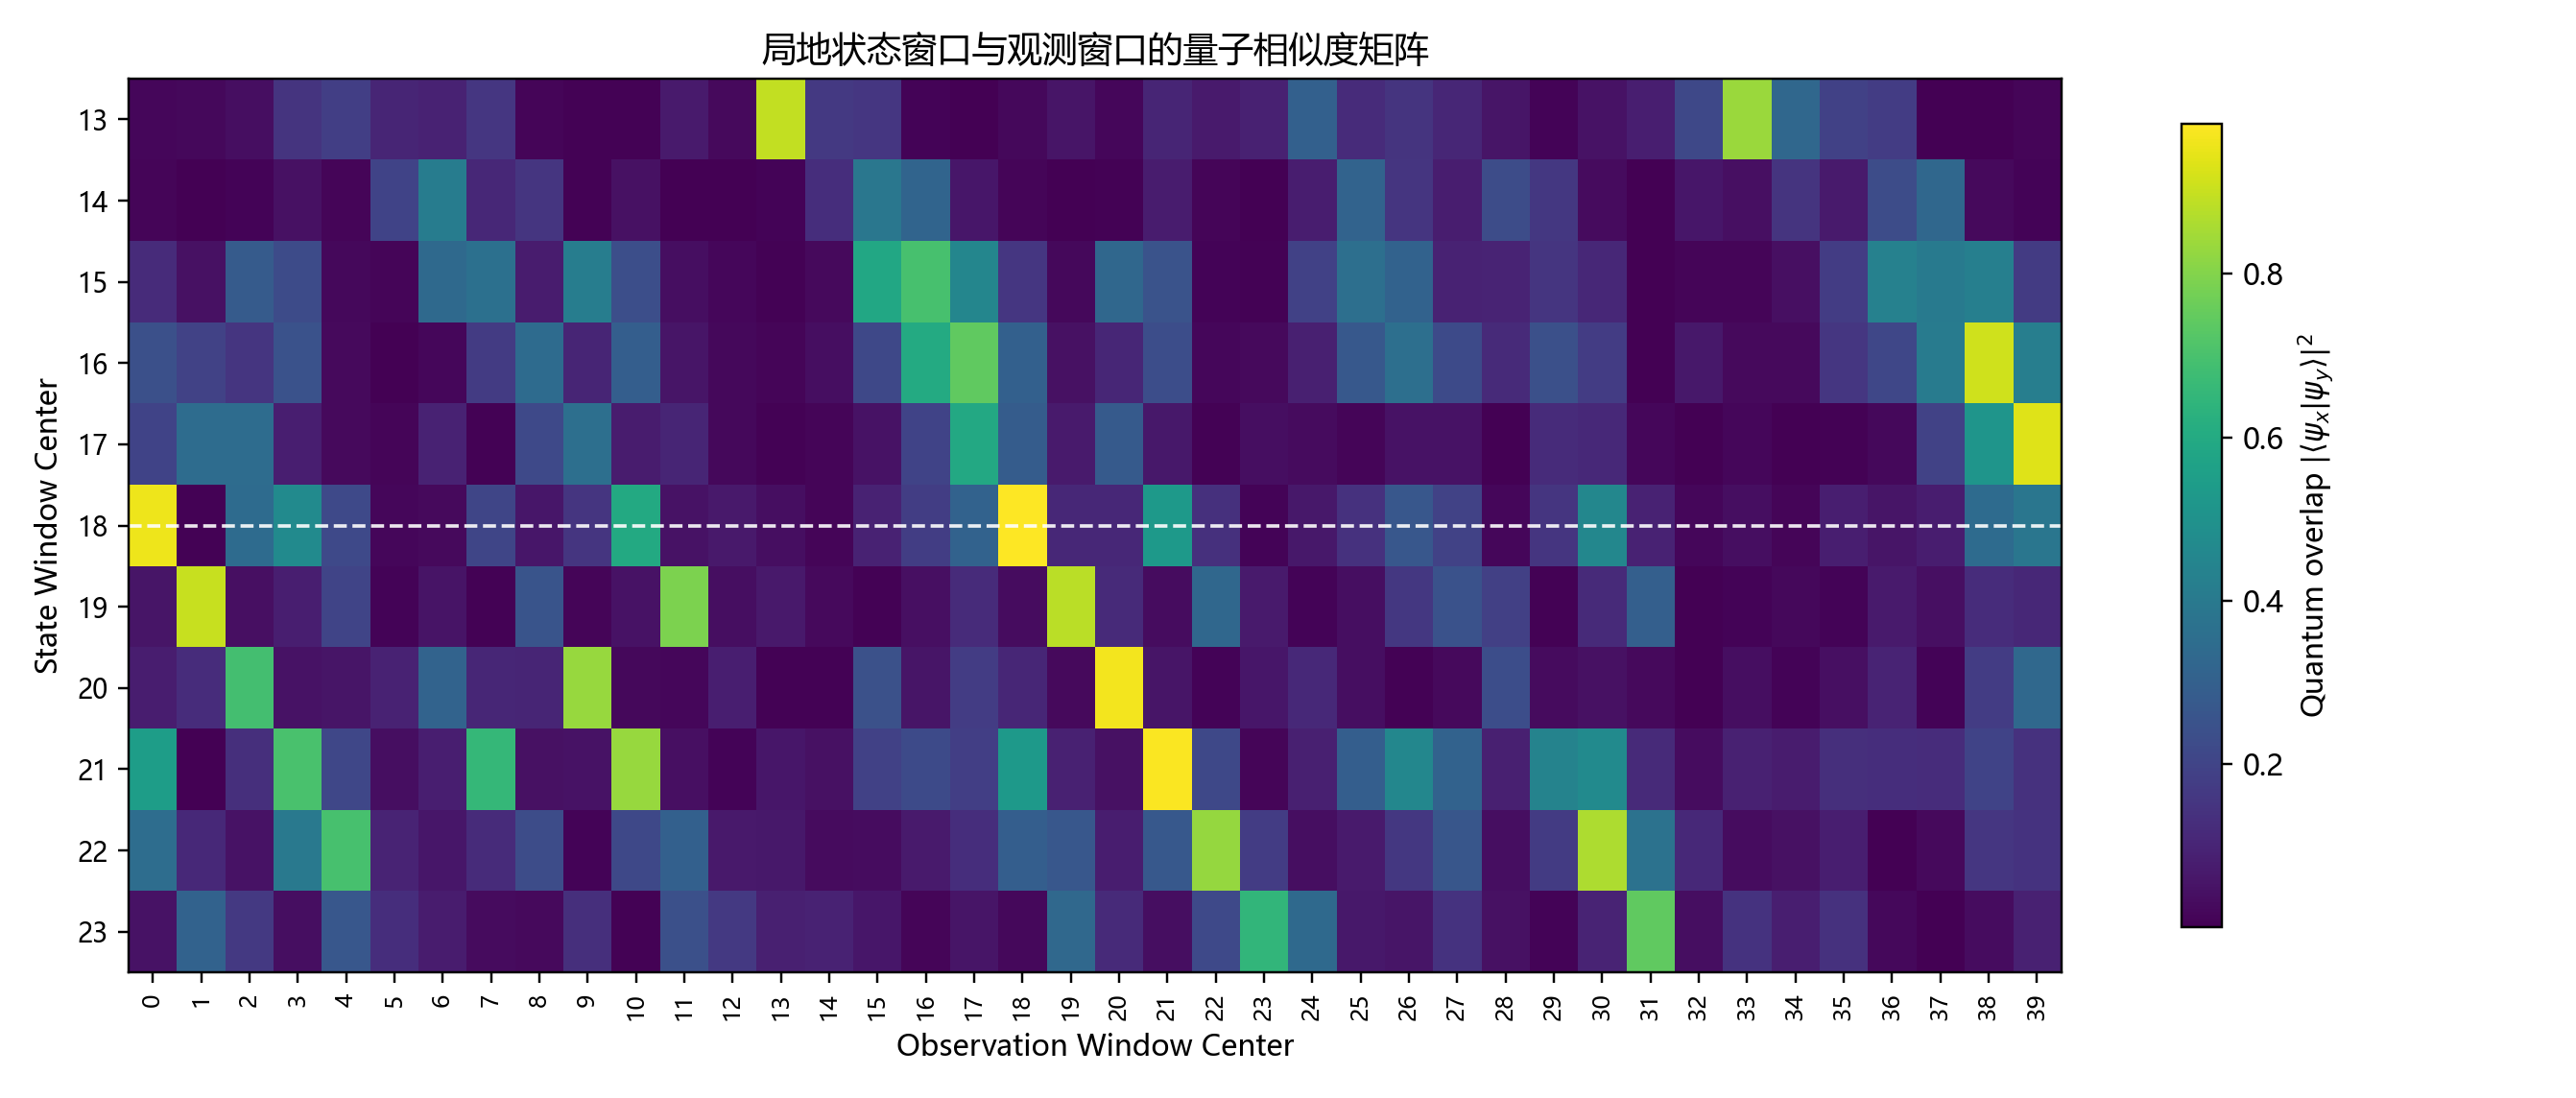
\includegraphics[width=0.92\linewidth]{figures/exp37_quantum_similarity_matrix.png}
\caption{代表性时间步下量子相似度的结构分布。}
\label{fig:qsim-innov}
\end{figure}

图 \ref{fig:qsim-innov} 进一步加强了这种解释性。该图显示，不同局地窗口之间的相似度并不是均匀或随机的，而是呈现出明显的块状和层次差异。这说明量子模块确实学习到了一种局地结构表达，而不是简单复述经典距离先验。若没有这层结构差异，后续的弱融合权重就不可能在保持稳定的同时提供额外信息。就本文当前实验而言，这种“结构表达创新”是有证据支持的；但是否能推广到更复杂系统和更大窗口，仍需后续工作检验。这里与现有量子核文献的关键差别在于，已有工作更多关注分类、回归或核分离能力\cite{yin2025photonicqkernel,saez2025qkernel}，而本文把量子相似度放进了局地同化加权这一更具体的动力系统任务中。

因此，本文的创新点可以进一步概括为三条解释链。第一条是“局地窗口解释链”，说明量子模块为何适合处理局地模式匹配；第二条是“相似度解释链”，说明量子特征映射为何能产生非平凡结构信息；第三条是“弱修正解释链”，说明这些结构信息为何必须以弱融合和弱 $J$ 修正的形式进入经典同化器。三条解释链共同决定了本文不是简单堆叠量子术语，而是在方法、结构和行为三个层次上都可解释。不过从学术表述上讲，本文更适合声称“在当前受控实验中建立了一套可解释的量子弱融合机制”，而不是直接宣称已经给出普适方法论。

\section{算法对比分析（如有，与常用量子算法或经典算法在性能、精度、资源消耗等方面的对比）}
与纯经典 fixed 基线相比，本文方法在保持 LETKF 主骨架稳定性的前提下，实现了更低的 test\_1 误差；与 corr 这类直接结构化加权方案相比，本文避免了强接入带来的明显退化。与常见“量子调参”思路相比，本文量子模块不只做外层搜索，而是直接参与局地相似度建模，因此更贴近“量子增强同化机制”本身\cite{felix2024reservoir}. 与 Kotsuki 等人的量子退火数据同化相比，本文不把 4D-Var 整体转化为量子优化问题，而是仅在 LETKF 的局地结构层引入量子信息\cite{kotsuki2024qda}；与物理驱动局部化工作相比，本文不是利用流场物理特征重设局部化函数，而是利用量子相似度重设局地观测加权\cite{sarp2025localization}。

从资源消耗上看，当前方法每次只需构造 $4$ qubits 局地特征映射电路，线路规模小、计算代价可控，适合在受限量子模拟环境下复现。其代价低于大规模全局量子化方案，也更符合赛题实际约束。

为了更清楚地体现本文方法与现有思路的差异，这里将对比分析拆成四个层面。第一层是与经典强基线的对比，回答“量子增强是否真的有额外价值”；第二层是与 corr 等结构化权重方法的对比，回答“为什么不是任何结构化加权都有效”；第三层是与物理驱动局部化或经验局地化修正路线的对比，回答“为什么本文选择量子相似度而不是纯物理特征”；第四层是与常见量子调参式思路或量子退火 DA 路线的对比，回答“量子模块究竟是在外层搜索、整体替代，还是在内层参与同化机制”。只有把这几个问题分开说明，才能体现本文方法的独特位置。

\begin{figure}[htbp]
\centering
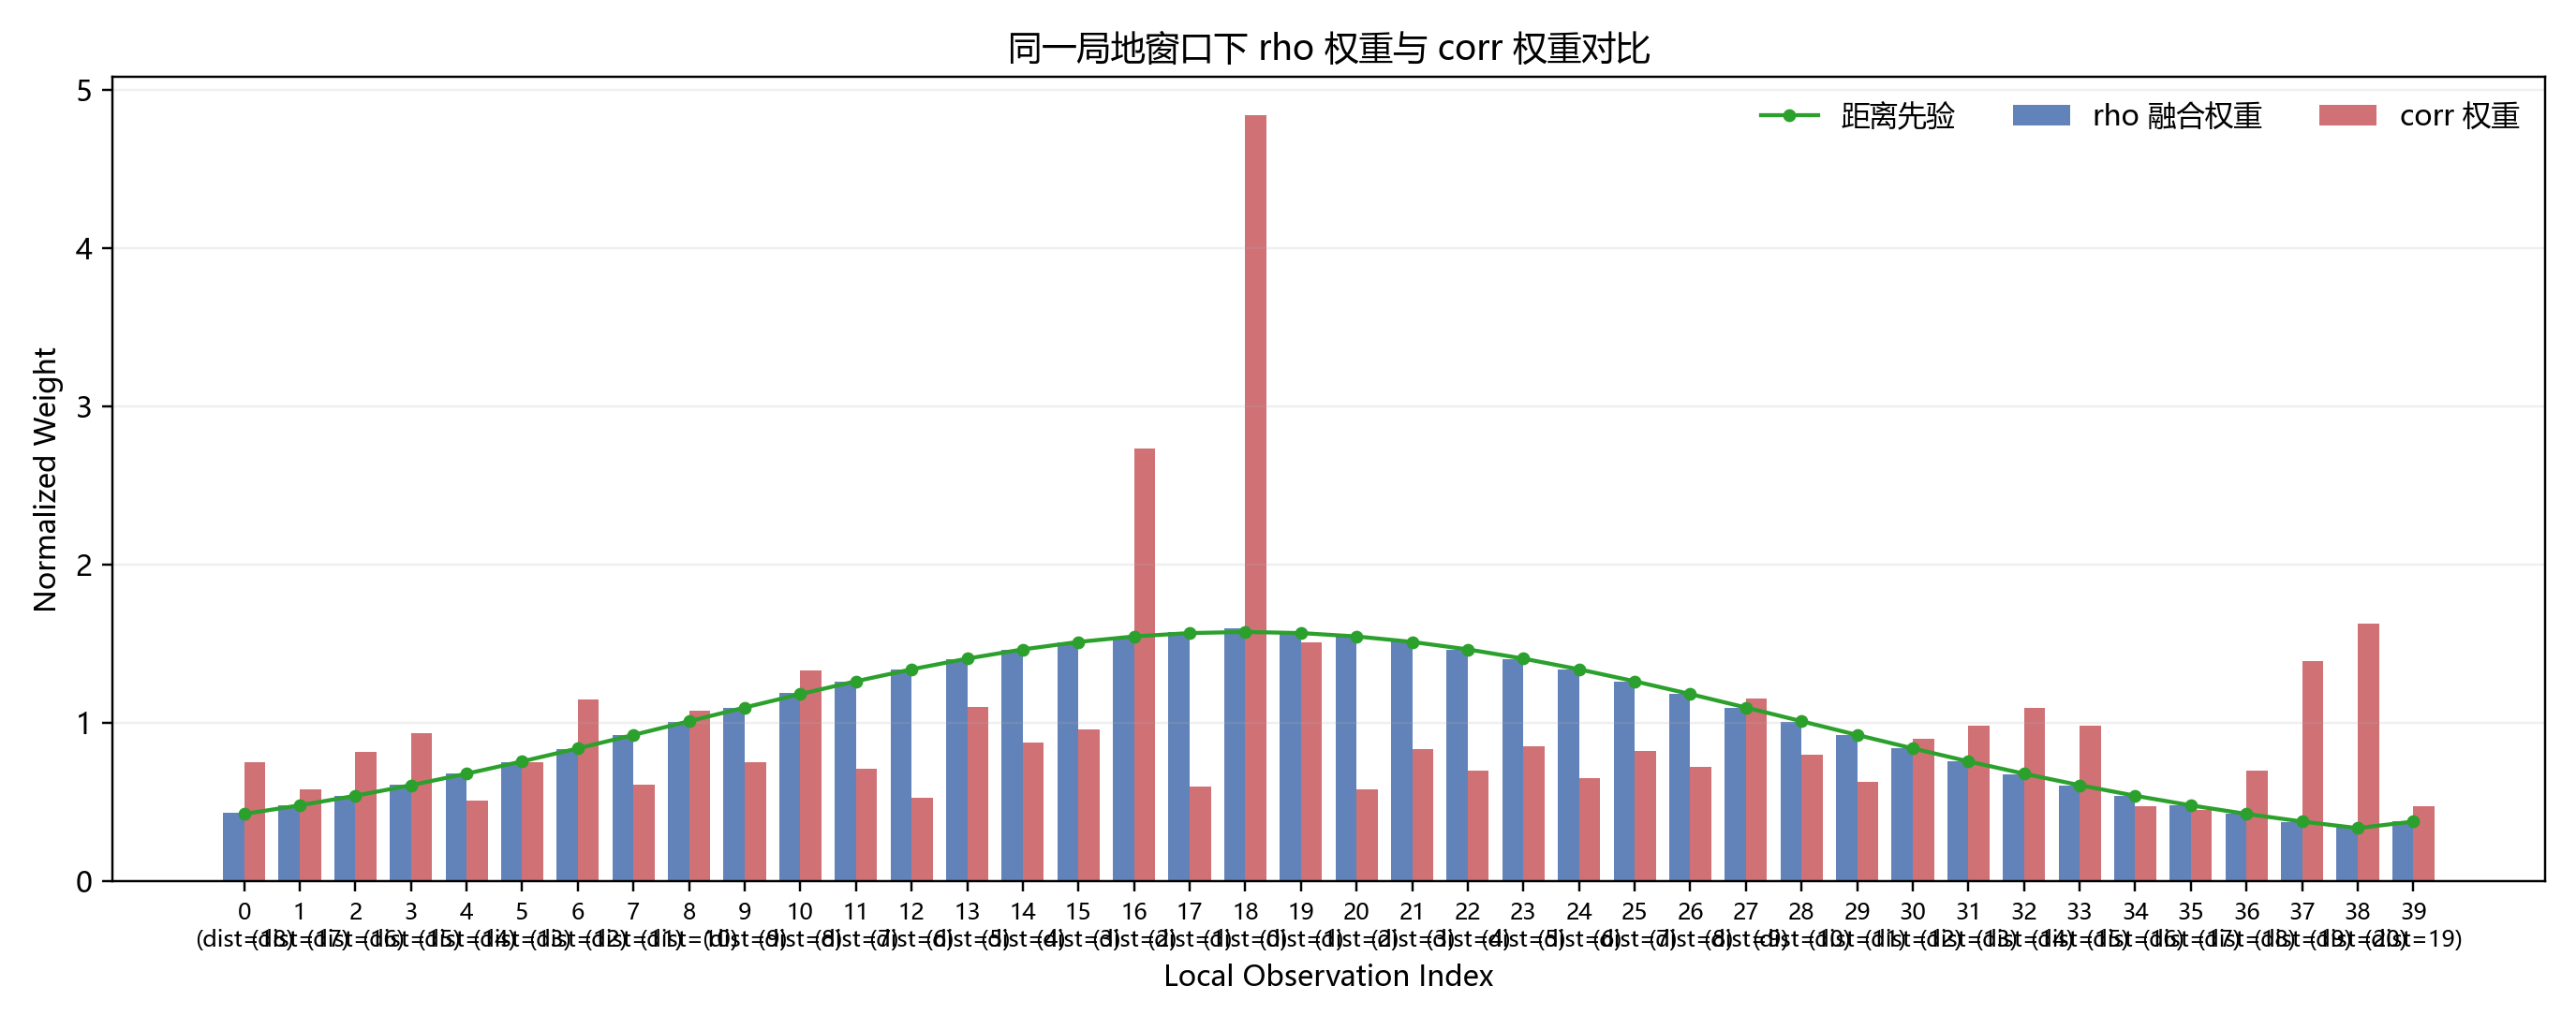
\includegraphics[width=0.92\linewidth]{figures/exp37_rho_vs_corr_weights.png}
\caption{同一局地窗口下，量子弱融合权重与 corr 权重的对比。}
\label{fig:weights}
\end{figure}

图 \ref{fig:weights} 进一步说明，本文方法与 corr 加权的差异不只是数值更优，而是机制不同。corr 权重更容易受局部相关性波动影响，而量子弱融合权重保留了距离先验，并用量子相似度做温和调制，因此整体更稳健。

换句话说，corr 更像是一种“单层直接加权”，而本文方法是一种“先保留经典局地结构，再叠加量子弱修正”的双层机制。这种差异决定了两者在稳定性上的表现不同：前者更容易因为局部相关性过强而退化，后者则更容易维持在可控的弱调制区间内。从数值上看，\texttt{corr} 的 test\_1 RMSE 为 $0.14279$，不仅没有优于 \texttt{fixed} 的 $0.12873$，反而恶化约 $10.93\%$；相比之下，最优量子弱融合配置为 $0.12698$，说明“结构化信息存在”并不自动意味着“任何结构化加权都有效”，关键仍在于结构信息如何进入经典更新。

\begin{figure}[htbp]
\centering
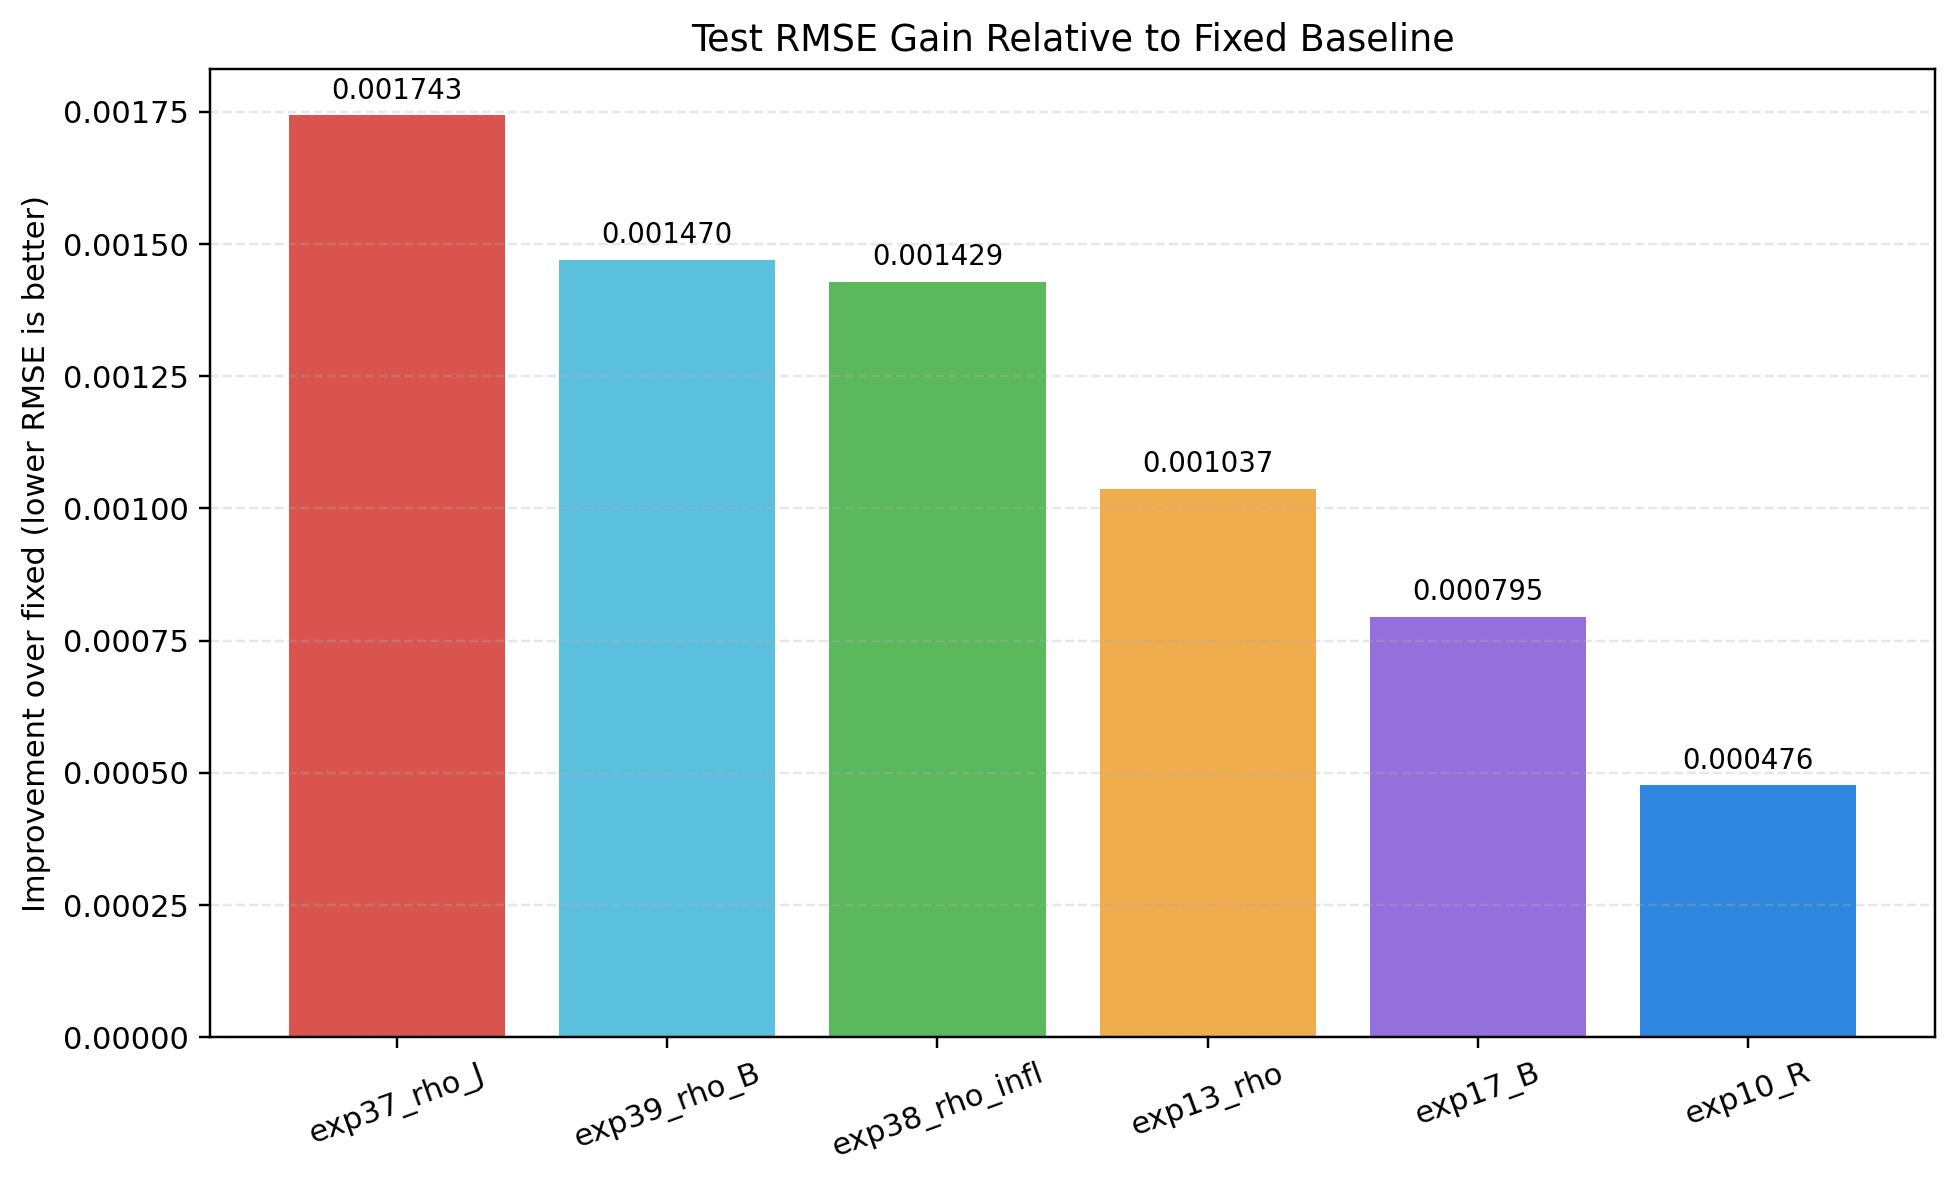
\includegraphics[width=0.92\linewidth]{figures/rmse_gain_over_fixed.png}
\caption{各候选高分方法相对 fixed 基线的 test\_1 RMSE 改善幅度。}
\label{fig:gain}
\end{figure}

图 \ref{fig:gain} 从更全局的候选方法角度补充了这一结论。该图展示了不同候选相对 fixed 的提升幅度，可以看到，在当前 exp37 全部六组受控配置里，四组量子弱融合都实现了正向改进，其中最优配置提升约 $1.35\%$，最弱配置也仍有约 $0.99\%$ 的提升。这说明本文的收益并非来自偶然挑中一个参数组合，而是来自对量子接入方式的有效筛选。

\begin{figure}[htbp]
\centering
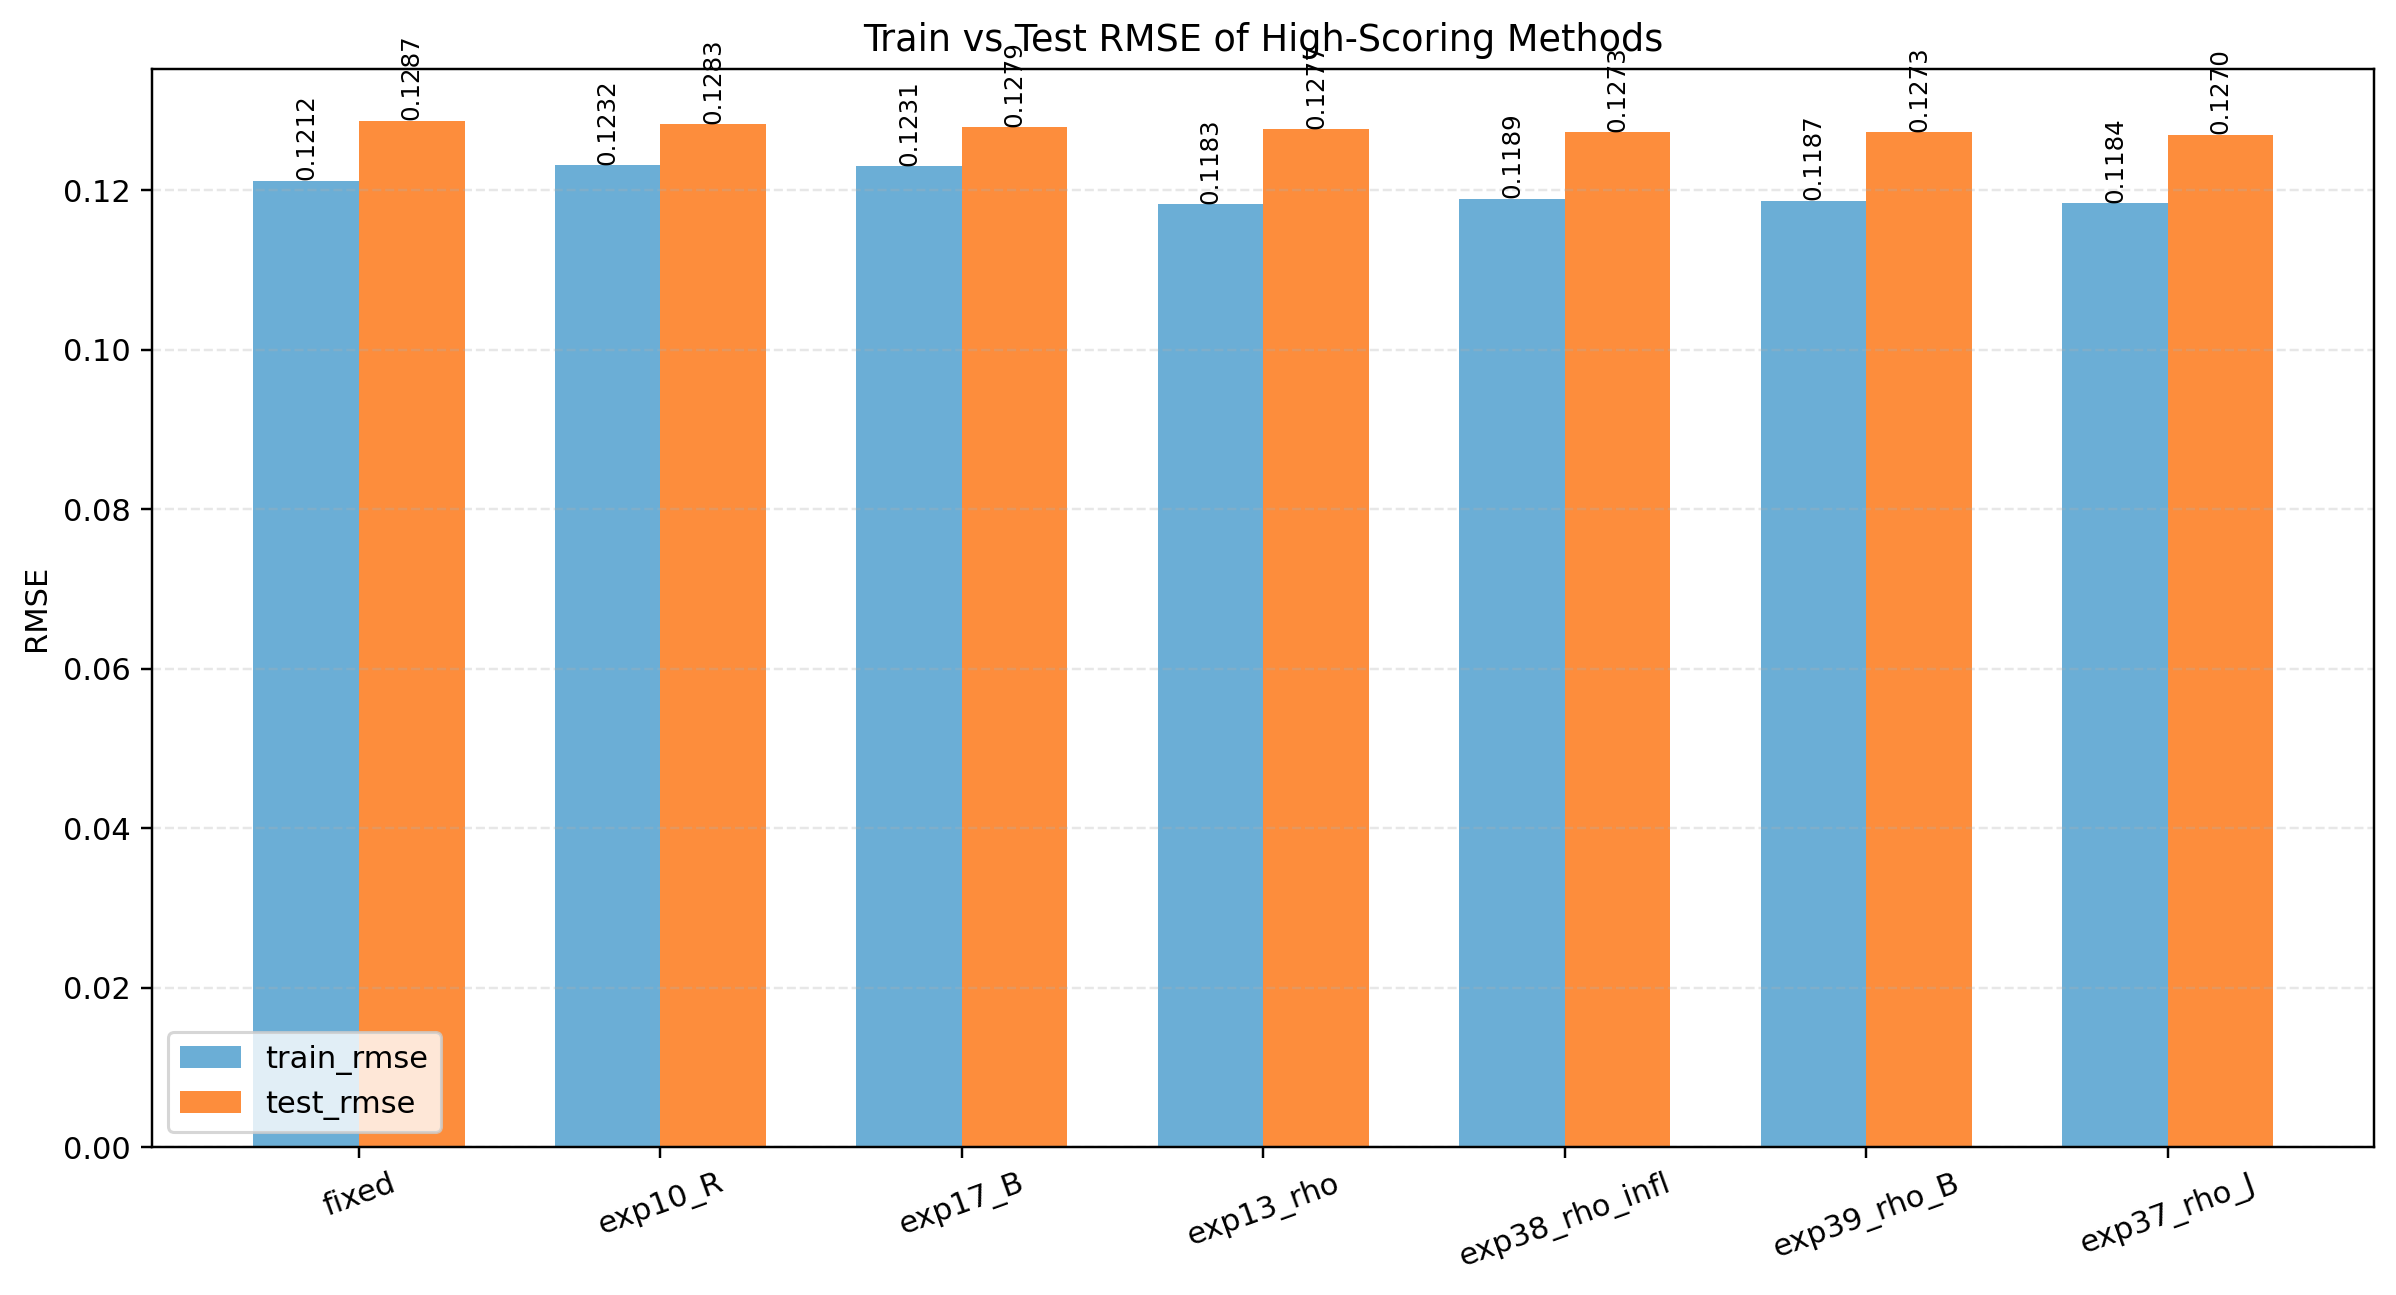
\includegraphics[width=0.92\linewidth]{figures/train_test_rmse_grouped.png}
\caption{高分候选方法在 train/test 上的 RMSE 分组对比。}
\label{fig:grouped}
\end{figure}

图 \ref{fig:grouped} 进一步说明，本文方法的优势并不只是训练端或局部测试端的偶然下降，而是在 train/test 两端都维持了较一致的表现。具体而言，最优量子弱融合配置的 train RMSE 为 $0.11844$，低于 fixed 的 $0.12120$；test\_1 RMSE 为 $0.12698$，同样低于 fixed 的 $0.12873$。对数据同化问题而言，这一点尤其重要，因为如果一个方法只在训练端改进明显、测试端退化，则说明它只是把局部结构拟合得更激进，而不具备真正的泛化能力。当前主线方案在这张图中的位置，更接近一种“稳健增益”而非“高风险高波动”方案。

\begin{figure}[htbp]
\centering
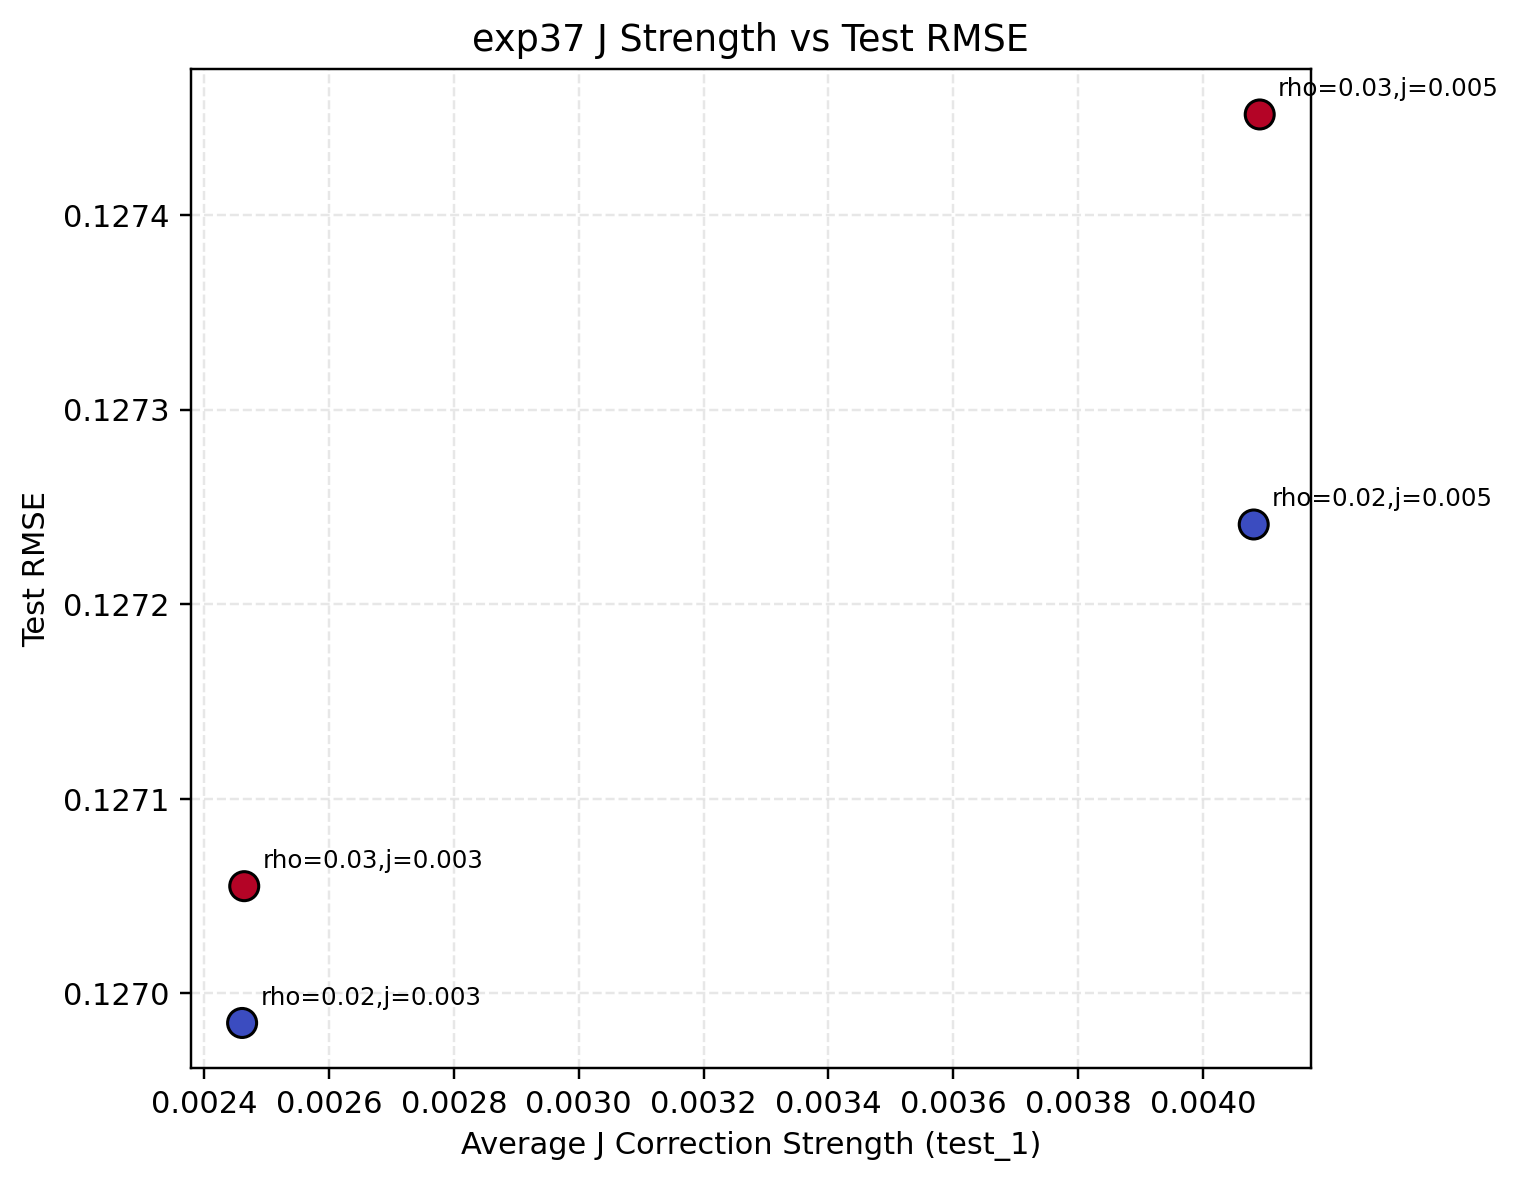
\includegraphics[width=0.92\linewidth]{figures/exp37_j_strength_vs_rmse.png}
\caption{平均 $J$ 修正强度与 test\_1 RMSE 的关系。}
\label{fig:jrmse}
\end{figure}

图 \ref{fig:jrmse} 则直接展示了本文思考过程中的一个关键结论：$J$ 修正并不是越强越好。当前网格中，当平均 $J$ 修正强度约为 $0.00246$ 时，test\_1 RMSE 最低；当其增加到约 $0.00409$ 时，test\_1 RMSE 升至 $0.12745$。这张图非常重要，因为它把“为什么本文坚持弱修正”从经验判断变成了可观察结论。也就是说，弱融合和弱 $J$ 修正不是保守写法，而是由实验行为本身支持的机制选择。

因此，本节对比分析最终支持四点判断。第一，本文方法优于纯经典 fixed，说明量子结构信息在当前受控实验里具有现实价值；第二，本文方法优于 corr 类直接加权，说明结构化信息只有以合适强度接入才有效；第三，本文与物理驱动局部化工作相似之处在于都试图摆脱固定经验局部化，但本文依赖的是量子相似度而不是显式流场特征\cite{sarp2025localization}；第四，本文不同于单纯量子调参或量子退火 DA，因为量子模块本身参与了局地结构建模与更新控制\cite{kotsuki2024qda,felix2024reservoir}。不过，受限于当前结果规模，本节更适合被视为“证据驱动的机制对比”，而不是对所有量子增强同化路线的全面定论。

\section{总结}
本文围绕“量子信息如何合理进入经典同化器”这一核心问题，给出了一组基于 Lorenz96 的量子弱融合受控实验。实验表明，量子结构本身并非无效，但若直接主导观测权重或分析更新，容易破坏经典同化的稳定性；相反，当其被解释为局地弱几何修正信号时，可以在保持 LETKF 稳定骨架的同时带来温和但可量化的收益。

因此，本文给出的主要结论不是“量子模块替代了经典同化器”，而是“在当前受控设定下，量子模块在局地结构建模和弱融合层面显示出一定现实价值”。从最终验证结果看，最优量子弱融合方案在 test\_1 上优于 fixed 基线，同时避免了 corr 方案的明显退化，说明“稳定骨架 + 局地弱修正”值得作为后续量子增强数据同化研究的一条候选方向。需要强调的是，本文的证据规模目前仍局限于单一 Lorenz96 设定、有限参数网格和单测试集比较，后续工作将进一步围绕更完整的验证划分、更丰富的中间消融、更稳定的量子表示层以及 gated/adaptive 变体的统一比较展开。

\section*{参考文献}
\begin{thebibliography}{99}

\bibitem{hunt2007letkf}
Hunt, B. R., Kostelich, E. J., \& Szunyogh, I. (2007).
Efficient data assimilation for spatiotemporal chaos: A local ensemble transform Kalman filter.
\textit{Physica D: Nonlinear Phenomena}, 230(1--2), 112--126.

\bibitem{kotsuki2024qda}
Kotsuki, S., Kawasaki, F., \& Ohashi, M. (2024).
Quantum data assimilation: a new approach to solving data assimilation on quantum annealers.
\textit{Nonlinear Processes in Geophysics}, 31, 237--245.

\bibitem{giannakis2022operator}
Giannakis, D., et al. (2022).
Data Assimilation in Operator Algebras.
\textit{arXiv preprint} arXiv:2206.13659.

\bibitem{calvello2025enkf}
Calvello, E., Reich, S., \& Stuart, A. M. (2025).
Ensemble Kalman methods: A mean field perspective.
\textit{Acta Numerica}, 34, 1--291.

\bibitem{felix2024reservoir}
Felix, O. A., Tennie, L., \& Magri, L. (2024).
Prediction of chaotic dynamics and extreme events: A recurrence-free quantum reservoir computing approach.
\textit{arXiv preprint} arXiv:2405.03390.

\bibitem{yin2025photonicqkernel}
Yin, Z., Agresti, I., de Felice, G., Brown, D., Toumi, A., Pentangelo, C., Piacentini, S., Crespi, A., Ceccarelli, F., Osellame, R., Coecke, B., \& Walther, P. (2025).
Experimental quantum-enhanced kernel-based machine learning on a photonic processor.
\textit{Nature Photonics}, 19, 1020--1027.

\bibitem{altmann2025qgk}
Altmann, P., Mansky, M. B., Zorn, M., Stein, J., \& Linnhoff-Popien, C. (2025).
Quantum Generator Kernels.
\textit{ICLR 2026 under review}. OpenReview: RbUe1cLXrJ.

\bibitem{saez2025qkernel}
S\'aez-Ortu\~no, L., Forgas-Coll, S., \& Ferrara, M. (2025).
Quantum Kernel Methods: Convergence Theory, Separation Bounds and Applications to Marketing Analytics.
\textit{arXiv preprint} arXiv:2510.11744.

\bibitem{sarp2025localization}
Er, S., \& Meldi, M. (2025).
Physics-based localization methodology for Data Assimilation by Ensemble Kalman Filter.
\textit{arXiv preprint} arXiv:2511.08845.

\bibitem{qtk2024}
Quantum tangent kernel. (2024).
\textit{Physical Review Research}, 6, 033179.

\bibitem{bansal2025qml}
Bansal, R., \& Rajput, N. K. (2025).
Quantum Machine Learning: Unveiling Trends, Impacts through Bibliometric Analysis.
\textit{arXiv preprint} arXiv:2504.07726.

\end{thebibliography}


\end{document}
